\documentclass[12pt, oneside, a4paper]{book}
\usepackage{setspace}
\usepackage{arabtex}
\usepackage{utf8} 
\usepackage{hyperref} 
\usepackage{graphicx}
\usepackage{subcaption}
\usepackage{geometry}
\usepackage{lipsum}
\usepackage{listings}
\usepackage{xcolor}
\usepackage{enumitem}
\usepackage{titlesec}
\usepackage{xparse}
\usepackage{verbatim}
\usepackage{float}
\usepackage{array}
\usepackage{ragged2e}
\usepackage{tabularx}
\usepackage{verbatimbox}
\usepackage{fancyhdr}
\usepackage{tocbibind}
\usepackage[toc]{appendix}
\usepackage[final]{pdfpages}


%
 \geometry{a4paper,inner=1.25in,outer=1.25in,top=1in,bottom=1in,footskip=15mm,headsep=30mm, headheight=-3mm}
% \renewcommand{\chaptermark}[1]{\markboth{\textit{\uppercase{chapter \thechapter. #1}}}{}}

\titlespacing*{\chapter}{0pt}{-\baselineskip}{1em}
\pagestyle{fancy} % Turn on the style
\renewcommand{\headrulewidth}{0pt}

\fancyhf{} % Start with clearing everything in the header and footer
\rhead{
	{\tiny 
		\RL{المملكة العربية السعودية} \\
		\RL{وزارة التعليم العالي} \\
		\RL{جامعة الأميرة نورة بنت عبد الرحمن} \\
		\RL{كلية علوم الحاسب والمعلومات} \\
		\RL{مشروع تخرج ١}}
}
\chead{
\includegraphics[width=.1\linewidth]{img/pnu.png}}
\lhead{
	{\tiny Kingdom of Saudi Arabia \\
		Ministry of Higher Education \\
		Princess Nourah bint Abdulrahman University \\
		Faculty of Computer \& Informaion Science \\
		Graduation Project I}
}
\cfoot{\thepage}%

\fancypagestyle{plain}
{
	\rhead{
		{\tiny \RL{المملكة العربية السعودية} \\
			\RL{وزارة التعليم العالي} \\
			\RL{جامعة الأميرة نورة بنت عبد الرحمن} \\
			\RL{كلية علوم الحاسب والمعلومات} \\
			\RL{مشروع تخرج ١}}
	}
	\chead{
\includegraphics[width=.1\linewidth]{img/pnu.png}}
	\lhead{
		{\tiny Kingdom of Saudi Arabia \\
			Ministry of Higher Education \\
			Princess Nourah bint Abdulrahman University \\
			Faculty of Computer \& Informaion Science \\
			Graduation Project I}
	}
	\cfoot{\thepage}%
}
\fancypagestyle{firstpage}
{
	\rhead{
		{\tiny \RL{المملكة العربية السعودية} \\
		\RL{وزارة التعليم العالي} \\
		\RL{جامعة الأميرة نورة بنت عبد الرحمن} \\
		\RL{كلية علوم الحاسب والمعلومات} \\
		\RL{مشروع تخرج ١}}
	}
	\chead{
\includegraphics[width=.1\linewidth]{img/pnu.png}}
	\lhead{
		{\tiny Kingdom of Saudi Arabia \\
		Ministry of Higher Education \\
		Princess Nourah bint Abdulrahman University \\
		Faculty of Computer \& Informaion Science \\
		Graduation Project I}
	}
}
\usepackage{xpatch}
\xapptocmd{\titlepage}{\thispagestyle{firstpage}}{}{}

\newcommand{\mychapter}[1]{\newpage%
	\thispagestyle{empty}
	\topskip0pt%
	\vspace*{\fill}%
	\addtocounter{chapter}{1}%
	\begin{center}%
		\textbf{\Large{\color{chapter}{CHAPTER NO. \thechapter \\ \uppercase{#1}}}}%
	\end{center}%
	\vspace*{\fill}%
	\addtocounter{chapter}{-1}
	\newpage%
	\chapter{#1}
}

\definecolor{chapter}{HTML}{773344}
\definecolor{section}{HTML}{f03a47}
\definecolor{sub}{HTML}{065143}
\definecolor{ssub}{HTML}{4381c1}
\definecolor{bold}{HTML}{cc3f0c}


\definecolor{lightgray}{HTML}{eeeeee}
\definecolor{darkgray}{rgb}{.4,.4,.4}
\definecolor{purple}{rgb}{0.65, 0.12, 0.82}
\definecolor{green}{rgb}{0,0.6,0}


\titleformat{\chapter}
{\color{chapter}\normalfont\Large\bfseries}
{\color{chapter}\thechapter}{1em}{}

\titleformat{\section}
{\color{section}\normalfont\fontsize{12}{16}\bfseries}
{\color{section}\thesection}{1em}{}

\titleformat{\subsection}
{\color{sub}\normalfont\fontsize{12}{14}\bfseries}
{\color{sub}\thesubsection}{1em}{}

\titleformat{\subsubsection}
{\color{ssub}\normalfont\fontsize{12}{13}\bfseries}
{\color{ssub}\thesubsubsection}{1em}{}


\newcommand{\code}[1]{{\color{red}\colorbox{lightgray}{#1}}}
\newcommand\boldcolor[1]{\textcolor{bold}{\textbf{#1}}}
\newcommand\Includegraphics[2][]{\addvbuffer[3pt 0pt]{\includegraphics[#1]{#2}}}

\lstset{frame=tb,
	language=Java,
	aboveskip=3mm,
	belowskip=3mm,
	showstringspaces=false,
	columns=flexible,
	basicstyle={\small\ttfamily},
	numbers=none,
	numberstyle=\tiny\color{gray},
	keywordstyle=\color{blue},
	commentstyle=\color{dkgreen},
	stringstyle=\color{mauve},
	breaklines=true,
	breakatwhitespace=true,
	tabsize=3
}
\setcounter{secnumdepth}{3}
\setcounter{tocdepth}{3}
\hypersetup{
	colorlinks,
	citecolor=[rgb]{0,0.5,0.5},
	filecolor=[rgb]{0,0.5,0.5},
	linkcolor=[rgb]{0,0.5,0.5},
	urlcolor=[rgb]{0,0.5,0.5}
}


\begin{document}
	\setcode{utf8}
	
	\pagenumbering{gobble}

	\begin{titlepage}
	%=========================
	\begin{center}
		\hspace{0pt}\\
		\vspace{4cm}
		{\scalebox{1}{\large\bfseries\color{section}\uppercase{Online Home Automation Control System}}}\\			
			\vspace{2cm}
			By: \\
			\begin{table}[H]
				\begin{center}
					\begin{tabular}{rl}		
						\texttt{436200058} & Abeer Ahmed Ezzat 
						\\
						\texttt{436200063} & Doha Nidal AlZouhbi
						\\
						\texttt{437004005} & Mona Saud AlKhathlan  
						\\
						\texttt{437004100} & Nouf Abdullah AlDajani 
						\\	
						\texttt{437004875} & Reem Ali AlGhamdi
						\\
						\texttt{436006939} & Sarah Khalid AlHussain 
					\end{tabular}
				\end{center}
			\end{table}
			
			Supervised By: \\
			\Large{Dr. Abeer Mahmoud}\\
			
			
			
			% ----------------------------------------------------------------
			\vfill \normalsize
			A Graduation Project Report Submitted to \\
			College of Computer and Information Sciences at PNU \\
			in Partial Fulfillment of the Requirements for the \\
			Degree of \\
			Bachelor of Science \\
			in \\
			Computer Sciences \\[5ex]
			CCIS, PNU \\
			Riyadh, KSA \\
			1440 - 1441H \\
			% ----------------------------------------------------------------
		\end{center}
	\end{titlepage}
	\newpage

	\addcontentsline{toc}{chapter}{\nameref{sec:ack}}
	\chapter*{Acknowledgment}
	\label{sec:ack}
	\paragraph{} First and foremost, we thank Allah the Almighty for always blessing us and for helping us complete this project on time. We would like to express our special thanks of gratitude to our project supervisor Dr. Abeer Mahmoud for her continuous support, motivation, and for always commenting on our best qualities and enhancing them. Without her direction and proper guidance, this project would not have succeeded. We thank her for her unwavering support. Not to forget our loving families and supporting friends for helping us sticking to the schedule. We also would like to thank Princess Nourah bint Abdulrahman University. Last but not least we want to thank anyone who has helped us by providing information, insight, comments or facilities that we needed to complete our project. Our heartfelt thanks to everyone we have mentioned.



	\pagenumbering{roman}

	%\addcontentsline{toc}{chapter}{Table of Contents}
	\tableofcontents
	\newpage	
	\doublespacing
	\newpage
	
	\listoftables
	\newpage
	
	\listoffigures
	\newpage
	
	\addcontentsline{toc}{chapter}{\nameref{sec:sym}}
	\chapter*{List of Symbols \& Abbreviations}
	\label{sec:sym}
	\def\arraystretch{1.5}
	\begin{table}[H]
		\begin{center}
			\begin{tabularx}{\linewidth}{|c|X|}\hline
				
				\boldcolor{Symbols \& Abbreviations} & \boldcolor{Meaning} \\\hline
				API & Application programming Interface\\\hline
				GPIO & General Purpose Input Output\\\hline
				GUI & Graphical User Interface\\\hline
				IDE & Integrated Development Environment \\\hline
				IoT & Internet of Things \\\hline
				JSON & JavaScript Object Notation\\\hline
				LED & Light Emitting Diode\\\hline
				REST & Representational State Transfer\\\hline
				SDLC & Software Development Life Cycle\\\hline
				SQL & Structured Query Language\\\hline
				UI & User Interface\\\hline
			\end{tabularx}
		\end{center}
		\caption{List of Symbols \& Abbreviations}
	\end{table}
	\newpage
	\addcontentsline{toc}{chapter}{\nameref{sec:kw}}
	\chapter*{Keywords}
	\label{sec:kw}
	\def\arraystretch{1.5}
	\begin{table}[H]
		\begin{center}
			\begin{tabularx}{\linewidth}{|c|X|}\hline		
				\boldcolor{Keyword} & \boldcolor{Definition} \\\hline
				Raspberry Pi & low cost, credit-card sized computer\cite{raspberry}. \\\hline
				Linear solenoid &  type of electromagnetic actuator that converts an electrical signal into a magnetic field producing a linear motion\cite{linear}.\\\hline				
			\end{tabularx}
		\end{center}
		\caption{Keywords}
	\end{table}
	\newpage
	\addcontentsline{toc}{chapter}{\nameref{sec:intro}}
	\chapter*{Abstract}
		\label{sec:intro}
		\paragraph{} The aim for this project is to control light buttons, air conditioners, television or other home appliance regardless of the person's location. The methodology is simple: an android app will send controlling requests to a web server. Raspberry Pi will be getting all the new requests from the server, processing it accordingly and controlling the hardware components connected to it. Such a system will allow someone in the United States to turn the lights in their house in Saudi Arabia on. However, an active connection to the internet must be present all the time. 
		
	

	\mychapter{Introduction}
		\pagenumbering{arabic}
		\section{Problem statement \& Significance}
		\paragraph{}With the recent very rapid progress in technology and automation, and towards easier daily life tasks, there has
		become a need for remote control of almost all possible aspects of living. Especially
		the house appliances that surround us,that allow focusing on main work of each day.
		\paragraph{}Some examples we have already encountered and used in our daily lives include using apps to control a cleaning robot or adjust the heating in the house or switch the house lights on or off. For the latter, there have been many applications that can do that. However, they all work in a small set of devices and sensors. It is necessary for such applications to exist, as a service like this would be important for many people. An example is working moms who are outside the house and want to switch the lights on at a certain time to wake their children up. Another example is pet owners who need to have UV lights switched on for their pets at certain times of the day but can’t do so immediately and so on. 
		\paragraph{}However, the main challenge in creating a device to solve this problem is where the idea of IoT (Internet of Things) comes in; learning how to control this device through the Internet from afar, rather than being controlled by infrared rays locally as is the case with most similar applications. 
		\section{Proposed Solution}
		\paragraph{}This project propose building an intelligent application that is based on IoT techniques. The created app should enable the user, by clicking on the appropriate buttons, to control a physical apparatus that needs to be pushed to work, such as lights buttons. This will be done by designing and creating an Android application, then using a small laptop, called Raspberry Pi, to control a small piece that will be pushed forward (on command) to switch the light on or off, the API is a web application hosted on a server.
		
		\subsection{Aims}
			\paragraph{}At the end of this project, we intend to achieve the following aims:
			\begin{itemize}
	 			\item Learn how to design a mobile application using previously learned and new knowledge
				\item Learn how to invoke a web API and use it in our application
				\item Learn Python programming language to control Raspberry Pi
				\item Learn Flask web micro-framework
			\end{itemize}
		\subsection{Goals}
			\paragraph{} At the end of this project, we expect to deliver:
			\begin{itemize}
				\item An Android application with a user friendly, simple, clear interface with buttons to control a LED and linear solenoid. However, theoretically, the system can accept any other electronic device as long as it can be installed in the electronic circuit. 
				\item A physical apparatus composed of the Raspberry Pi connected to and controlling the piece.
				\item A web application following REST architecture, managing user  requests and Raspberry Pi's responses.
			\end{itemize}
		\section{Project Domain \& Limitation}
			\subsection{Domain}
				\paragraph{} Although the application will be available for all kinds of users to use, we expect that the ones who would make the most use of it would be people who have some background in electrical engineering and computer science. 
			\subsection{Limitation}
			\paragraph{} This project aims to control any hardware connected to the electronic circuit. Thus, the flexibility and freedom are extremely high. However, this advantage comes at a non-financial cost: the learning curve. The users must be knowledgeable about the basics of electrical engineering and computer science. A manual could be made to make the process easier.
		\section{Gantt Chart}
		\begin{figure}[H]
			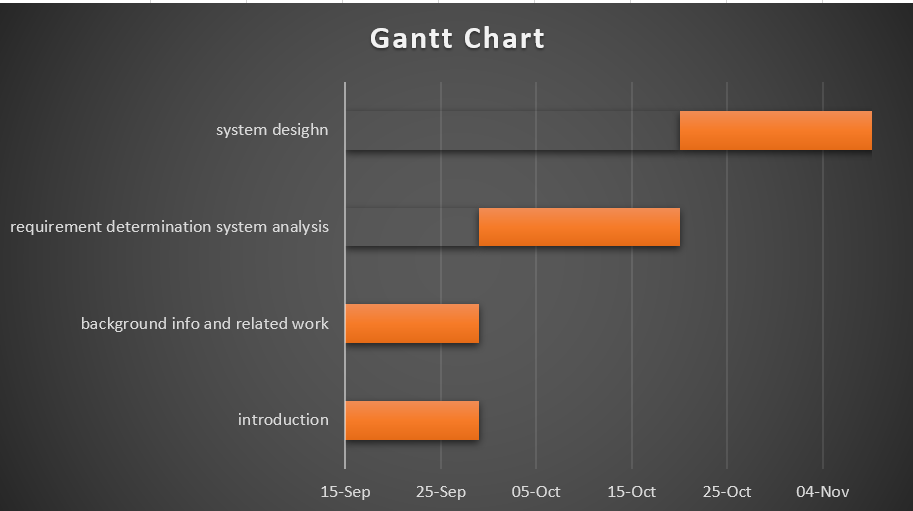
\includegraphics[width=\linewidth]{img/gantt_chart.png}
  			\caption{Gantt Chart}	
	\end{figure}
		\newpage	
		\mychapter{Background Information \& Related Work}
			\section{Background Information}
			\subsection{IoT}
			\paragraph{}The internet of things (IoT) is one of the most important technological developments in the last decade. Do you wonder were the term IoT came from? It was coined by Kevin in 1999 \cite{iot_1}. This means we can describe IoT as the ability to connect as many things by the internet without humans’ help by using technologies such as cloud computing, Radio Frequency Identification (RFID), wireless communication, sensors, Internet protocol, ultra-low-power processors and others \cite{iot_3}.
			\subsubsection{IoT Architecture}
			\paragraph{} It is basically what IoT is made of. It contains three layers; Perception layer, Network layer, and Application layer. So, to know these layers better we need to know the definition of them.
			\begin{itemize}
				\item \boldcolor{Perception layer:} is responsible for perceiving and identifying objects or things in the environment \cite{iot_4}.
				\item \boldcolor{Network layer:} is responsible for receiving and transmitting data between layers \cite{iot_5}.
				\item \boldcolor{Application layer:} is the interface for all previous layers used to process and transport data to provide services to the users \cite{iot_6}.
			\end{itemize}
			\subsubsection{IoT Applications}
			\paragraph{}There are different kinds of applications that make life easier and more secure. These are some example of them:
			\begin{itemize}
			\item \boldcolor{Automobiles:}  by IoT technology, it makes cars smarter and works to improve safety on the road by helping cars detect obstacles and assist braking or adapt their speed to the flow of traffic. Also it helps protect the environment by reducing fuel consumption, etc \cite{iot_7}.
			\item \boldcolor{Smart Home:}  You can control your entire home with a touch screen or your smartphone whether you are inside or outside a home, for example, you can lock or open your doors, turn on/off the light and air conditioner, etc \cite{iot_8}.
			\item \boldcolor{Healthcare:} IoT has an important role in healthcare applications by providing the ability to easily monitor and manage patient health without having to manually visit each patient the doctor can give a remote diagnosis to provide quality care more quickly and manage the health care environment more efficiently \cite{iot_5}.
			\end{itemize}
			\subsection{Hardware}
				\begin{itemize}
				\item \boldcolor{Raspberry Pi:} a small general purpose computer. All hardware components will be connected to it. An active connection to the internet is needed for it to fetch data from the server\cite{raspberry}. %insert figure here% 
				\item \boldcolor{Ubuntu Web Server:} hosts the web application. Digital Ocean severs\cite{digital_ocean} were chosen for this project.
				
				\item \boldcolor{LED:} since the hardware components controlled depends heavily on the user needs, this project main aim will be controlling a small LED. LED stands for light-emitting diode\cite{led}. Basically a small light source. %insert figure here% %
				\item \boldcolor{Linear Solenoid:} once the LED works, linear solenoid will be installed for demonstrating the idea\cite{linear}. It is a small component that generates a linear motion. It will be used to press in anything, such as lights, TV remote, and coffee machine. %insert figure here%
				\end{itemize}
				
			\subsection{Programming Languages \& Frameworks}
				\begin{itemize}
					
					\item \boldcolor{Python:} raspberry pi can be controlled by either c++ or python. Python was chosen because a REST API can be made using it fast.
		 				\begin{itemize}
		 					\item \textbf{GPIO:} a library for controlling any hardware component connected to the GPIO pins\cite{gpio}.
		 					\item \textbf{Flask:} a lightweight framework to build web applications.
						\end{itemize}
					\item \boldcolor{Java:} mobile application are made in a native way with either swift or java.
						\begin{itemize}
							\item \textbf{Android:} a framework for making android apps.
							\item \textbf{Retrofit:} type-safe HTTP client for Android and Java\cite{retro}. It will be used to send and receive commands and status from the web server.
							
						\end{itemize}
					\item \boldcolor{PostgreSQL:} an open-source RDBMS\cite{postgres}. It will be installed on the server.
				\end{itemize}
			
			\subsection{SDLC Model}
			\paragraph{} Incremental model will be used in this project. This model is a process of software development where requirements are broken down into multiple standalone modules of software development cycle. Incremental development is done in steps from analysis design, implementation, testing / verification, maintenance\cite{sdlc}. The reason this model was chosen is the pieces will be installed, tested and connected to the system gradually. First a LED, then a linear solenoid and so on.
			
			
		\newpage	
		\section{Related Work}
		\subsection{Insteon - Insteon Hub}
		\begin{figure}[H]
			
\includegraphics[width=\linewidth]{img/insteon.png}
  			\caption{Related Work: Insteon}
  			\label{related:insteon}
		\end{figure}
		\paragraph{}Insteon Hub is a simple and straightforward system that connects you to your home from any smartphone or tablet, anywhere in the world. Control Insteon light bulbs, wall switches, outlets, and thermostats at home or remotely and receive instant email or push notification alerts from motion, door and window, water leak, and smoke sensors while you’re away\cite{insteon}. \textit{Figure \ref{related:insteon} shows the home page for Insteon}.
		\begin{itemize}
		\item \boldcolor{Advantage:}
			\begin{enumerate}
				\item Control Multiple Devices Simultaneously with a Basic Scene.
				\item Create Schedules to Turn Your Lights On and Off at Specific Times.
				\item Automatically Turn Lights On and Off with Sensors.
				\item Monitor Your Home with Email or Push Notification Alerts.
			\end{enumerate}
		\item \boldcolor{Disadvantage:} 
			\begin{enumerate}
				\item Hub setup takes a couple of minutes and a few moments per light switch, sensor.
				\item Its need to connect it to power and your home's internet router so if the internet die all devices need to start over again. 
				\item fixed the hub take more cost than its original price.
				\item There is no database save/restore. You have to recreate all the devices, scenes, schedules if its replaced.
			\end{enumerate}
		\end{itemize}
		\newpage	
		\subsection{Wink - Wink Hub 2}
		\begin{figure}[H]
  			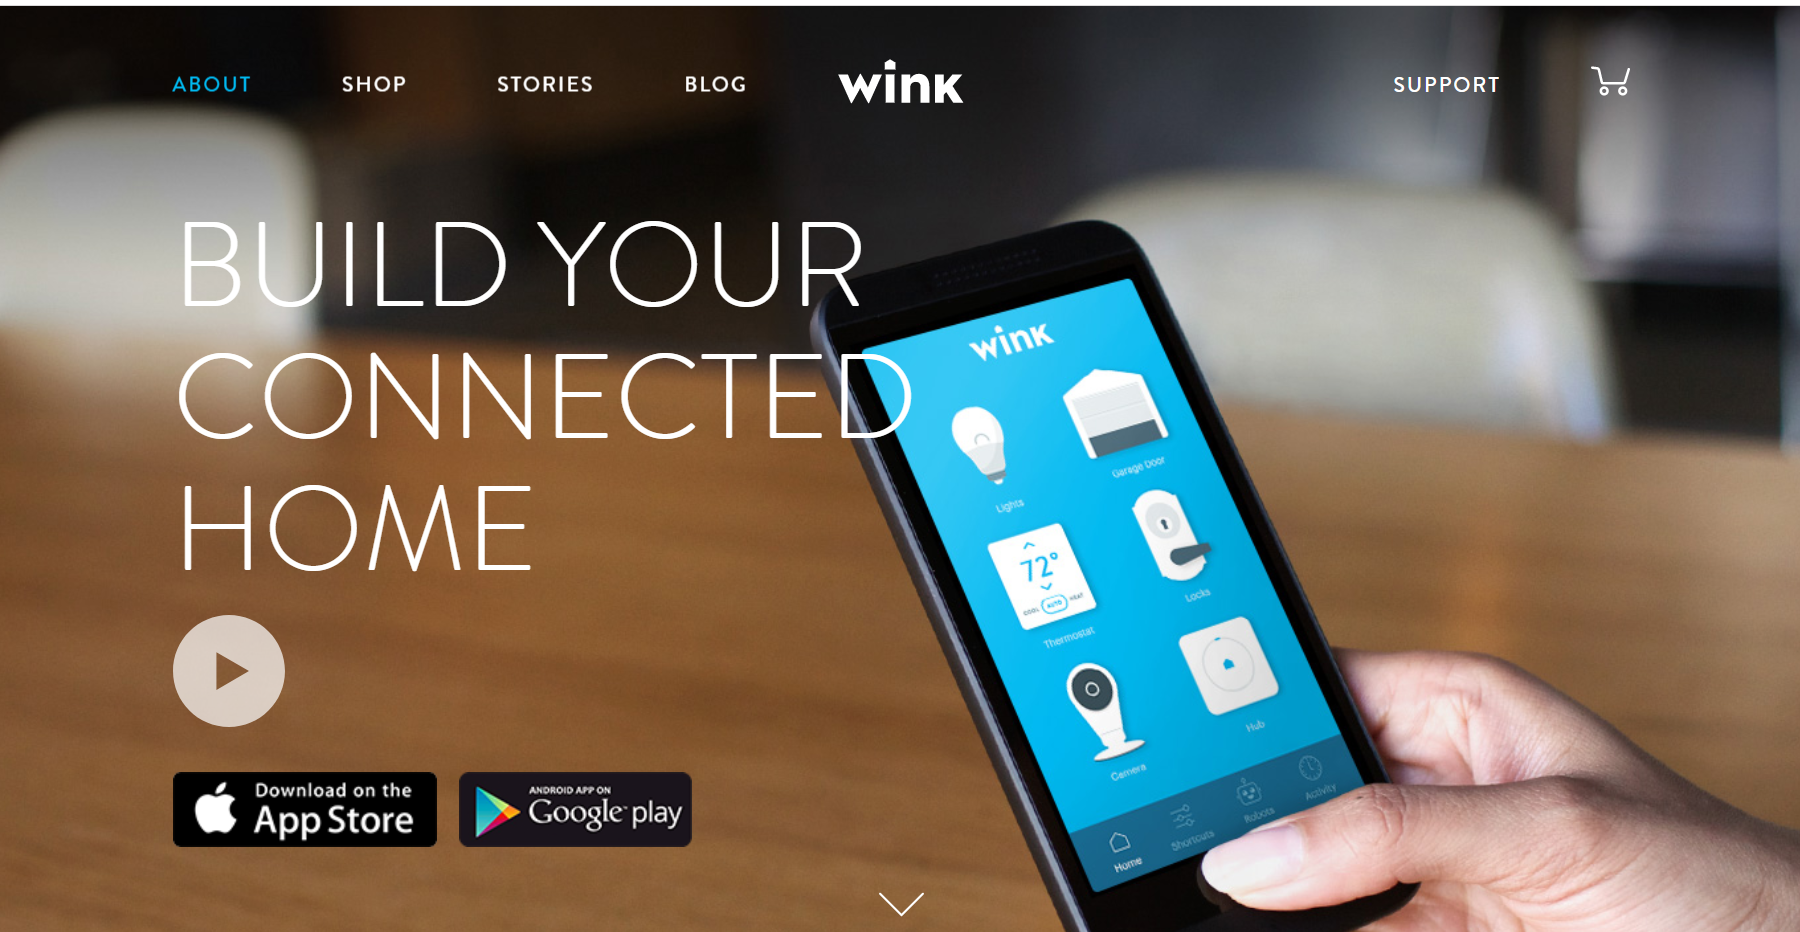
\includegraphics[width=\linewidth]{img/wink.png}
  			\caption{Related Work: Wink}
  			\label{related:wink}
		\end{figure}
		\paragraph{}Wink Hub 2 is the world’s first smart home hub created for the mainstream consumer. With industry-leading smart home protocol support, enhanced connectivity features, and a sleek design, Wink Hub 2 brings hundreds of products from best-in-class brands together for a simple, intuitive experience\cite{wink}. \textit{Figure \ref{related:wink} shows the home page for Wink}.
		
		\begin{itemize}
			\item \boldcolor{Advantage:}
			\begin{enumerate}
				\item Support Different platforms such as iOS or Android.
				\item Once you've created an account, Wink has the ability to recognize the products within Wink Bright, guide you through a few simple steps, and then you're ready to go.
				\item Wink works with Cortana Microsoft’s voice assistant and Amazon Alexa.
				\item One Important features in wink, its can see what you’re spending even before the bill arrives.
			\end{enumerate}
			\item \boldcolor{Disadvantage:} 
			\begin{enumerate}
				\item One major problem with the Wink 2 hub is that the device sometimes loses connectivity and must be reset in order for it to connect again.
				\item Wink app doesn't always let you access other devices' full features.
				\item High price.
				\item Takes 14 days to arrive.
			\end{enumerate}
		\end{itemize}
		\newpage
		\subsection{Samsung – Smart Things Hub}
		\begin{figure}[H] 			
			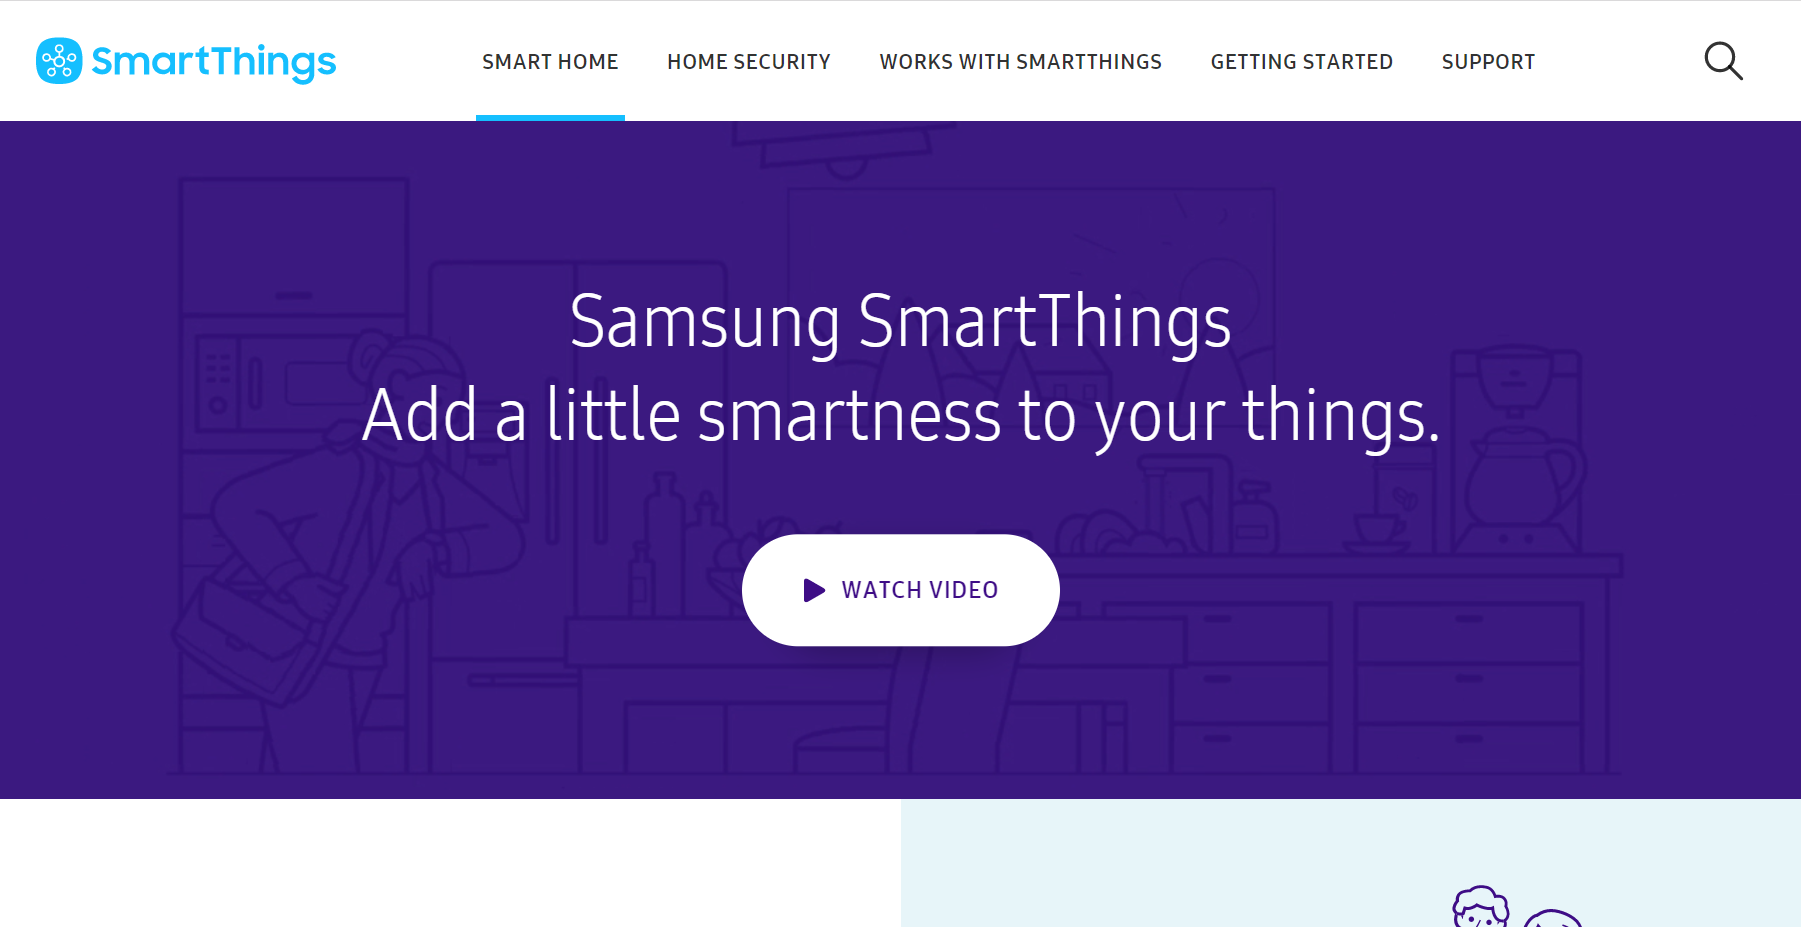
\includegraphics[width=\linewidth]{img/samsung.png}
			\caption{Related Work: Samsung}
			\label{related:samsung}
		\end{figure}
		\paragraph{}Smart things hub Connect wirelessly with a wide range of smart devices and make them work together\cite{samsung}. \textit{Figure \ref{related:samsung} shows the home page for Samsung}.
		\begin{itemize}
			\item \boldcolor{Advantage:}
			\begin{enumerate}
				\item Monitor and control connected devices in your home using a single SmartThings app for iPhone or Android.
				\item Manage connected devices in your home with SmartThings Routines for Good Morning, Goodbye, Good Night, and more.
				\item Receive alerts from connected devices when there’s unexpected activity in your home.
				
			\end{enumerate}
			\item \boldcolor{Disadvantage:} 
			\begin{enumerate}
				\item Some compatible components may not work as efficiently or smoothly as you want them to, which may be inconvenient.
				\item Some users report it stops working at times.
				\item Difficult to upgrade from older hub.
				\item In US Only.
			\end{enumerate}
		\end{itemize}
		\section{Proposed \& Similar System Comparison}
			\def\arraystretch{1.5}
			\renewcommand\tabularxcolumn[1]{>{\Centering}m{#1}}
			\begin{table}[H]

			\begin{center}
			\begin{tabularx}{1\linewidth}{|m{2.2cm}*4{|X}|}\hline
					
					& \boldcolor{Raspberry Pi} & \boldcolor{Insteon} & \boldcolor{Wink hub 2} & \boldcolor{Samsung (smart things)}  \\\hline
					
					\boldcolor{design} &
						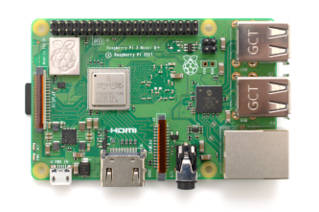
\includegraphics[width=\linewidth]{img/raspberry.png} &
						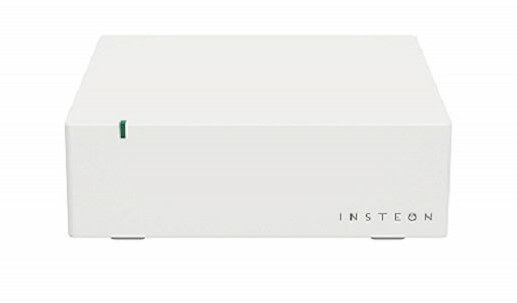
\includegraphics[width=\linewidth]{img/insteon_hw.png} & 
						\Includegraphics[width=\linewidth]{img/wink_hw.png} &
						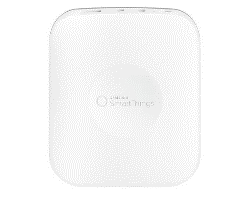
\includegraphics[width=\linewidth]{img/samsung_hw.png}
					 \\\hline

					\boldcolor{Hub Price} & 25\$ & 80\$ & 99\$ & 70\$ \\\hline
					\boldcolor{Hardware Price} & parts are very cheap &  expensive parts & very expensive parts & expensive parts \\\hline
					\boldcolor{Flexibility} & any hardware that can be physically connected & 42 hardwares of basic variety\cite{insteon_p} & 102 hardwares of different variety\cite{wink_p} & only 6 hardwares support \cite{samsung_p} \\\hline
					
					\boldcolor{Installation \& Configuration Difficulty} & require one expert user. Easy control for all other users via mobile app & easy to install and control hardwares with mobile app  &easy to install and control hardwares with mobile app  & easy to install and control hardwares with mobile app
					\\\hline
				\end{tabularx}
			\end{center}
			\caption{Proposed \& Similar System Comparison}
		\end{table}
		\textit{Better quality can be found at Appendix \ref{appendix:similar_system_comparision}}
		\newpage
		\paragraph{} Although similar systems already exists, our system has its own special advantages. The biggest being \textbf{hardware freedom}. In other systems, there exists a main hub receiving user command from the mobile app. So far, the ideas and implementation is identical. The previous systems require the consumer to by additional parts for it to work, such as special LED lights that needs installation or a small component controlling air conditioners. Those parts are usually limited in numbers, usage and can get very expensive fast. On the other hand, our system works with any hardware component as long as connecting it to the electrical circuit is possible.
		\paragraph{} However, this great flexibility comes with a great sacrifice: the steep learning curve. To keep the hardware prices as low as possible while maintaining high flexibility requires the buyer household to have one expert user. For example, in a family of four, all can control the AC. However, one of them must be an expert who can configure the hardware controlling the AC and adding it to raspberry pi manually. Of course, making it easier is possible, but it will result in a higher component cost and less flexibility as hardware components would need to be bought from our company (future implementation) in comparison to buying it from any cheap electronic store (current proposed solution).
		\paragraph{} \textit{figure \ref{fig:radar_diagram}} shows this relationship between flexibility, cost and usability for the three systems, our proposed solution and the merchant edition(future work).
		\begin{figure}[H]
			\centering
			\begin{subfigure}[b]{.4\linewidth}
				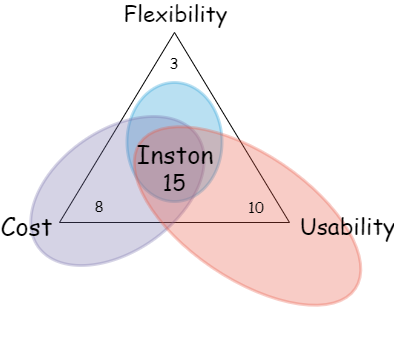
\includegraphics[width=\linewidth]{img/Inston.png}
				\caption{Insteon}
			\end{subfigure}
			\begin{subfigure}[b]{.4\linewidth}
				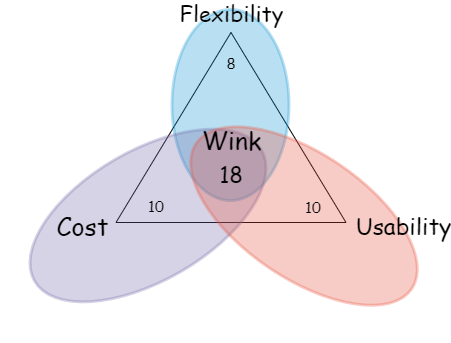
\includegraphics[width=\linewidth]{img/Wink.png}
				\caption{Wink}
			\end{subfigure}
			\begin{subfigure}[b]{.4\linewidth}
				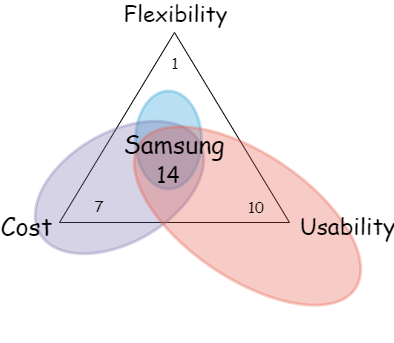
\includegraphics[width=\linewidth]{img/Samsung.png}
				\caption{Samsung}
			\end{subfigure}
			\begin{subfigure}[b]{.4\linewidth}
				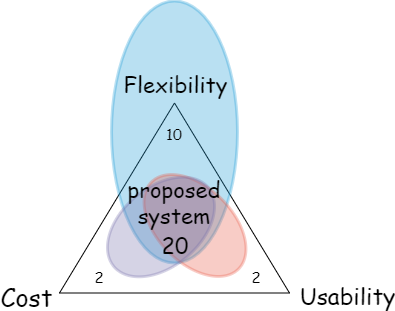
\includegraphics[width=\linewidth]{img/proposed.png}
				\caption{Proposed System}
			\end{subfigure}
			\begin{subfigure}[b]{.4\linewidth}
				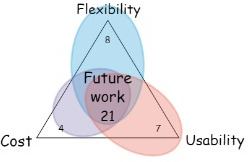
\includegraphics[width=\linewidth]{img/future.jpg}
				\caption{Future Work}
			\end{subfigure}
		
			\caption{Relationship between cost, flexibility and usability}
			\label{fig:radar_diagram}
		\end{figure}
	\mychapter{System Analysis}
		\section{Requirement Specification}
			\subsection{Overview}
				\paragraph{} The proposed project consists of three main systems: the android application which will be the user interface, the Raspberry Pi, which is the small computer where all the hardware pieces will be connected to, and the web server which will host the REST web application and be the connection between the android application and the Raspberry Pi.
				
				\paragraph{}First, the user is required to install the android app on his mobile phone. When the app is opened, the user either register or login. Once logged in, a list of raspberry pis is shown with the possibility of adding more. To add a new raspberry pi, the user must scan the QR code that belongs to the raspberry pi. Any user or raspberry added is immediately uploaded to the web server.
				
				\paragraph{}Once a raspberry is clicked, an activity displaying the hardwares that are connected to the Raspberry Pi is shown. It gets this list of hardwares from the webserver by using the GET method. When the user clicks on any  hardware that is there, a new activity opens. In it is mentioned the name of the hardware, the status (e.g. whether it is on or off), the commands and the scheduling configuration. All of this information is obtained from the server. 
				
				\paragraph{}Next to the commands title, there will be a small button that when clicked on will open a third activity, which gives the option of adding a new command. The command can be instantaneous (for example, switching an LED light immediately) or it can be scheduled for a later date or time. For the instantaneous command, the POST method will be used, and for scheduling the commands, the user will have the option to choose the date and time he wishes the commands to be undertaken in. Whatever the outcome of this process is, a popup message will appear to the user either confirming the success of the command the user issued, or denying it while explaining the reason for that failure.
				
				\paragraph{}Under the commands tab, there will be a  configuration 	section where all the scheduled commands will appear, along with their dates and times and options to edit them or delete them. The edit option will be done by the PUT method and the deleted option by the DELETE method. All the methods work on the data in the server’s database i.e. they either add a new command (POST), edit a scheduled command (PUT), or delete an existing command (DELETE). 
				
			
				\paragraph{}For the Raspberry Pi, the sequence it works according to is timed. Every 5 minutes, it puts the hardware status to the server so that it can show on the user’s application hardware list. Also, every 30 seconds, it checks the server for any new commands posted by the user from the android application. If there are any new ones that have to be, it updates its own local database (a local queue) according to the priorities and scheduled dates and times of the commands. This local database is organized according to the time the command was issued (i.e. the instantaneous commands are put at the front of this queue because of their precedence and the scheduled ones are put in the command order) and contains the command ID, which hardware this command was issued for, when this command was issued, and whether the command was successfully done or not, all gotten from the server by the GET method except the “successfully done” column, which the Raspberry edits according to the hardware. 
				
				\paragraph{}Whatever the result of the command was, the Raspberry posts the response of the command to the server. The android application gets this response from the server every 5 or 10 minutes, depending on the user’s choice. The response is displayed as a push notification in the user’s mobile phone. Depending on this response, the status and configuration information in the app will be updated to reflect the success or failure of the command response. Finally, it is important to note that any new hardware or configuration added to or connected to the Raspberry will have its information posted to the server by the Raspberry computer, where the user can view it then as soon as he opens his application to the first activity. When the response is successfully done and read by the user, the webserver deletes it from the database to save space. The webserver also deletes instantaneous commands once the user is notified the execution result. 
				\subsubsection{Input}
				The user command issued using the Android client is the main input. Each command consist of the following:
				\begin{itemize}
					\item chosen hardware.
					\item configuration wanted.
					\item optional scheduling information.
				\end{itemize}
				The \textbf{hardware} is the physical component connected to raspberry pi. Each hardware has a set of possible states that it can be in. Those states are called \textbf{configuration}. The \textbf{schedule} indicates the time of day and days of week the user might want the command to run at.
				\subsubsection{Output}
				\begin{itemize}
					\item a response
				\end{itemize}
				The raspberry pi issues a \textbf{response} indicating whether the command has been successfully done with an optional message. This response is saved in the webserver, which in turn is read by the android client periodically.  
			
		\newpage\section{Requirement Analysis}
			\subsection{Software Requirements}
			\begin{itemize}
				\item \boldcolor{Languages}
				\begin{itemize}
					\item Java
					\item Python
					\item SQL
				\end{itemize}
				
				\item \boldcolor{Frameworks \& libraries}
				\begin{itemize}
					\item Android
					\item Retrofit
					\item GPIO
					\item Flask
					\item SQLAlchemy
				\end{itemize}

				\item \boldcolor{IDE}
				\begin{itemize}
					\item Android studio
					\item Pycharm
				\end{itemize}

				\item \boldcolor{Databases}
				\begin{itemize}
					\item Postgresql
					\item Sqlite
				\end{itemize}
			
				\item \boldcolor{Web Server}
				\begin{itemize}
					\item Nginx
					\item uWsgi
				\end{itemize}
			\end{itemize}
			\newpage\subsection{Hardware Requirements}
				\begin{itemize}
					\item \boldcolor{Raspberry Pi} 
					\begin{itemize}
						\item Raspberry Pi 3 B+.
						\item a minimum of 2 GB of RAM.
						\item a minimum of 10 GB space in SD card.
						\item a monitor, a keyboard and a mouse, alternatively SSH connection could be established.
						\item internet connection, either via Wi-Fi or Ethernet cable.
						\item breadboard, cables, and resistors for circuit.
						\item RGB LED, solenoid, or any other hardware components satisfying user needs.
					\end{itemize}
					\item \boldcolor{Server} 
					\begin{itemize}
						\item Ubuntu 16.04+ server, we chose digital ocean's. The web server and database server shall be installed here.
						\item Minimum of 1GB of RAM.
						\item Minimum of 10GB of available space.
					\end{itemize}
					\item \boldcolor{Android mobile phone} 
				\end{itemize}
			\newpage\subsection{Functional Requirements}
			\renewcommand{\labelenumii}{\theenumii}
			\renewcommand{\theenumii}{\theenumi.\arabic{enumii}.}
				\begin{enumerate}[label=3.2.3.\arabic*]
					\item \boldcolor{Expert User's Functionalities:}
					\begin{enumerate}
						\item Expert user shall be able to add new hardware to the system. %A
						\item Expert user shall be able to add new configuration to the system. %A
					\end{enumerate}
					\item \boldcolor{Android Client's Functionalities:}
					\begin{enumerate}
						\item Android client shall allow user to login or register
						\item Android client shall allow user to add a new raspberry pi to the system
						\item Android client shall allow user to remove a raspberry pi from the system
						\item Android client should get hardware list from webserver. %M
						\item Android client should get scheduled commands from webserver. %M
						\item Android client shall be able to submit a new a command, might be scheduled, to webserver. %N
						\item Android client shall be able to delete a scheduled command from webserver. %N
						\item Android client shall be able to edit a scheduled command from webserver. %D
						\item Android client shall get responses from webserver automatically. %D
					\end{enumerate}
					\item \boldcolor{Raspberry pi's Functionalities:}
					\begin{enumerate}
						\item Raspberry pi should get command list each 30 seconds. %S
						\item Raspberry pi shall be able to update local queue. %S
						\item Raspberry pi shall execute commands saved in queue. %R
						\item Raspberry pi shall be able to submit a command response to server. %R
					\end{enumerate}
					\item \boldcolor{Web application's Functionalities:}
					\begin{enumerate}
						\item Web application should delete executed immediate commands. %N
						\item Web application should delete read responses. %S
					\end{enumerate}
				\end{enumerate}
			\newpage\subsection{Non-Functional Requirements}
				\def\arraystretch{1.5}
				\begin{table}[H]
					\begin{center}
						\begin{tabularx}{\linewidth}{|c|X|}\hline
							\boldcolor{Requirement} & \boldcolor{Description}\\\hline
							\textbf{Availability} & The system shall not be shut down for maintenance for more than 1 minute. \\\hline
							\textbf{Usability} & Except the expert user, all other user of the system shall be able to use the system immediately without much training  \\\hline
							\textbf{Verifiability} & The system shall check the user identity. \\\hline
							\textbf{Performance and Delay} & The raspberry pi shall read user commands each 30 seconds to avoid delay or overhead in the system\\\hline
							\textbf{Flexibility} & Any hardware component, such as linear solenoid or an infra-red controller, can be added to the system as long as it can be connected to the electric circuit.  \\\hline
							\textbf{Security} & Each user can only communicate with assigned raspberry pi. In a similar manner, raspberry pi only reads commands meant for it and not for other ones.  \\\hline
							\textbf{Efficiency} & The web server cleans the database and deletes any unneeded rows routinely.  \\\hline
						\end{tabularx}
					\end{center}
					\caption{Non-functional requirements}
					\label{table:non-func}
				\end{table}
			\paragraph{} \textit{Table \ref{table:non-func}} shows the non-functional requirements for the system and their description. The most important requirement is flexibility, as it is the core feature differentiating the proposed system from other systems. Next comes security and verifiability. They guarantee that no intruders are going to interrupt the system even if they communicated with the REST API directly without the android app because they won't be authorized -or authenticated- to enter the system. The other requirements are manly for performance and ease of use. 
			\newpage\subsection{Structured Diagrams}
				\subsubsection{Use Case Diagram}
				\paragraph{} \textit{Figure \ref{fig:diagram_usecase}} shows the use-case diagram of the system. Although the system learning curve is steep, each raspberry pi can be connected to multiple users and vice versa -i.e. many to many relationship-. In other words, in a household of four people, all of them can connect to the same raspberry and control the AC. However, only one of them must be knowledgeable about the basics of electrical engineering and computer science. This person is referred to as the \textbf{Expert User}. All other users including the expert user are referred to as \textbf{Users}. 
				 In this system, there are four main actors:
				\begin{itemize}
					\item \boldcolor{User}: any person using the system. They don't have to have any kind of background information at all. All they need to do is install the android app and clicks buttons on it. 
					\item \boldcolor{Expert user}: a type of user than configure the raspberry pi. They must manually connect the hardware to the GPIO pins, add it to the database and configure it. 
					\item \boldcolor{Android client}: the android application that the user uses. The android app makes requests and takes responses from the web server either by user order, such as deleting a certain command, or by itself such as getting the raspberry pi responses from the webserver periodically. 
					\item \boldcolor{Raspberry Pi}: the computer controlling the hardwares. It communicates with the web server to get the commands periodically then executes it.
				\end{itemize}
					\begin{figure}[H]
					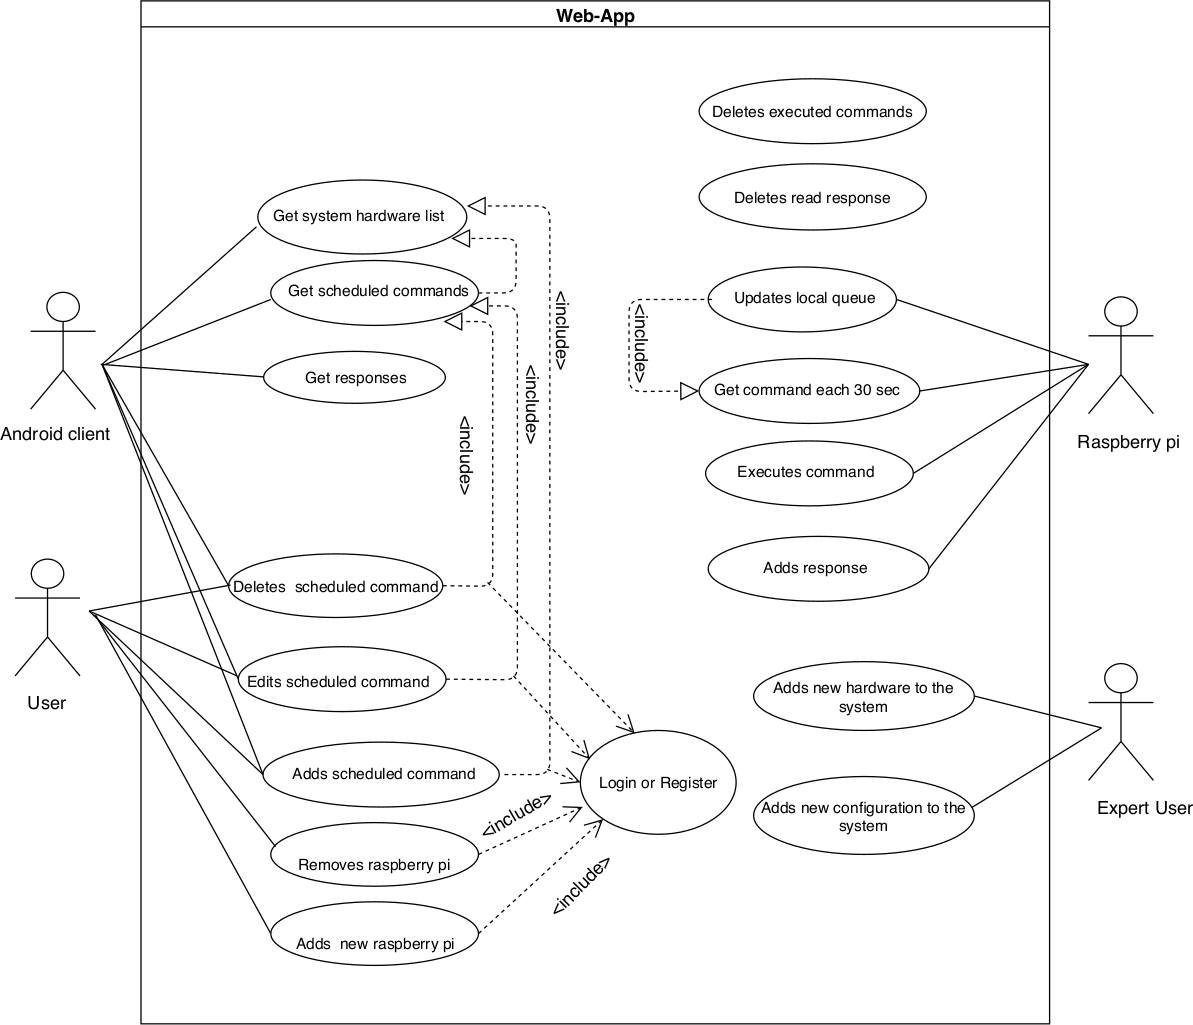
\includegraphics[width=\linewidth]{img/diagram_usecase.png}
					\caption{Use case diagram}
					\label{fig:diagram_usecase}
					\end{figure}
				
				\newpage\subsubsection{Use Case Scenarios \& Sequence Diagrams}
				\boldcolor{Expert user adds a new hardware to system}
				\newline\textbf{Sequence diagram:} \textit{Figure \ref{admin_hw}}
				\newline\textbf{Goal:} to add a new hardware device that the user can control to the Raspberry Pi.
				\newline\textbf{Actors:} Expert user, Raspberry Pi, Web server.
				\newline\textbf{Precondition:} None.
				\newline\textbf{Primary Scenario:}	
				\begin{enumerate}[label*=\arabic*.]
					\item Expert user physically connects the new hardware to the Raspberry Pi
					\item Expert user inserts new hardware attributes into hardware table in the raspberry local database. 
					\item Raspberry pi uploads information to the webserver using \textit{POST} \code{/hardware}
				\end{enumerate}
				\textbf{Variant:}\newline
				\hspace*{5mm}1.A. A physical defect might appear in the new hardware, the wires connecting it to the Raspberry Pi, or its ports, all resulting in the new hardware not working correctly. \\
				\begin{figure}[H]
					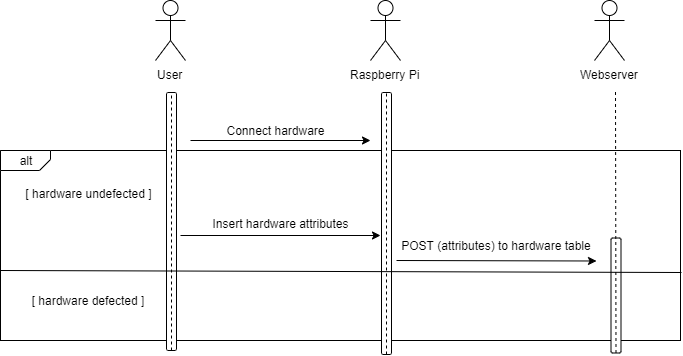
\includegraphics[width=\linewidth]{img/sequence_add_hardware.png}
					\caption{sequence diagram: Expert user adds a new hardware to system}
					\label{admin_hw}
				\end{figure} 
				\newpage\hspace*{-6mm}\boldcolor{Expert user adds a new configuration to system}
				\newline\textbf{Sequence diagram:} \textit{Figure \ref{admin_config}}
				\newline\textbf{Goal:} to add a new configuration to a new hardware.
				\newline\textbf{Actors:} Expert user, Raspberry Pi, Web server.
				\newline\textbf{Precondition:} Hardware has been added to the system successfully.
				\newline\textbf{Primary Scenario:}	
				\begin{enumerate}[label*=\arabic*.]
					\item Expert user inserts new configuration attributes into configuration table in the raspberry local database. 
					\item Raspberry pi uploads information to the webserver using \textit{POST} \code{/configuration}
				\end{enumerate}
				\textbf{Variant:}\newline
				\hspace*{5mm}1.A. A physical defect might appear in the new hardware, the wires connecting it to the Raspberry Pi, or its ports, all resulting in the new hardware not working correctly. \\
				\begin{figure}[H]
					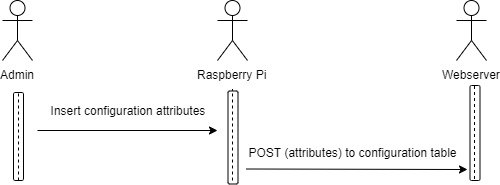
\includegraphics[width=\linewidth]{img/sequence_add_config.png}
					\caption{sequence diagram: Expert user adds a new configuration to system}
					\label{admin_config}
				\end{figure}
				%%%
				\newpage\hspace*{-6mm}\boldcolor{User login or register}
				\newline\textbf{Sequence diagram:} \textit{Figure \ref{user_login}}
				\newline\textbf{Goal:} to login a user if exists, or make a new user otherwise.
				\newline\textbf{Actors:} Android app, Web server.
				\newline\textbf{Precondition:} user opens android app.
				\newline\textbf{Primary Scenario:}	
				\begin{enumerate}[label*=\arabic*.]
					\item android app prompt user to enter credentials.
					\item android POST data to webserver's endpoint \code{/login} 
					\item web app checks email and password. If the user already exists and credentials are correct, return token. If the the user doesn't exist create user and return token.
					\item Android calls web server's endpoint \code{/raspberry} using the token in the authorization header to get the list of raspberry pi's related to the user
					\item Android display this array to user in UI.
				\end{enumerate}
				\textbf{Variant:}\newline
				\hspace*{5mm}*. user might exit android app. \\
				\hspace*{5mm}2.A. android app might fail to connect to the internet \\
				\hspace*{5mm}3.A. email might not match password, return error message \\
				\begin{figure}[H]
					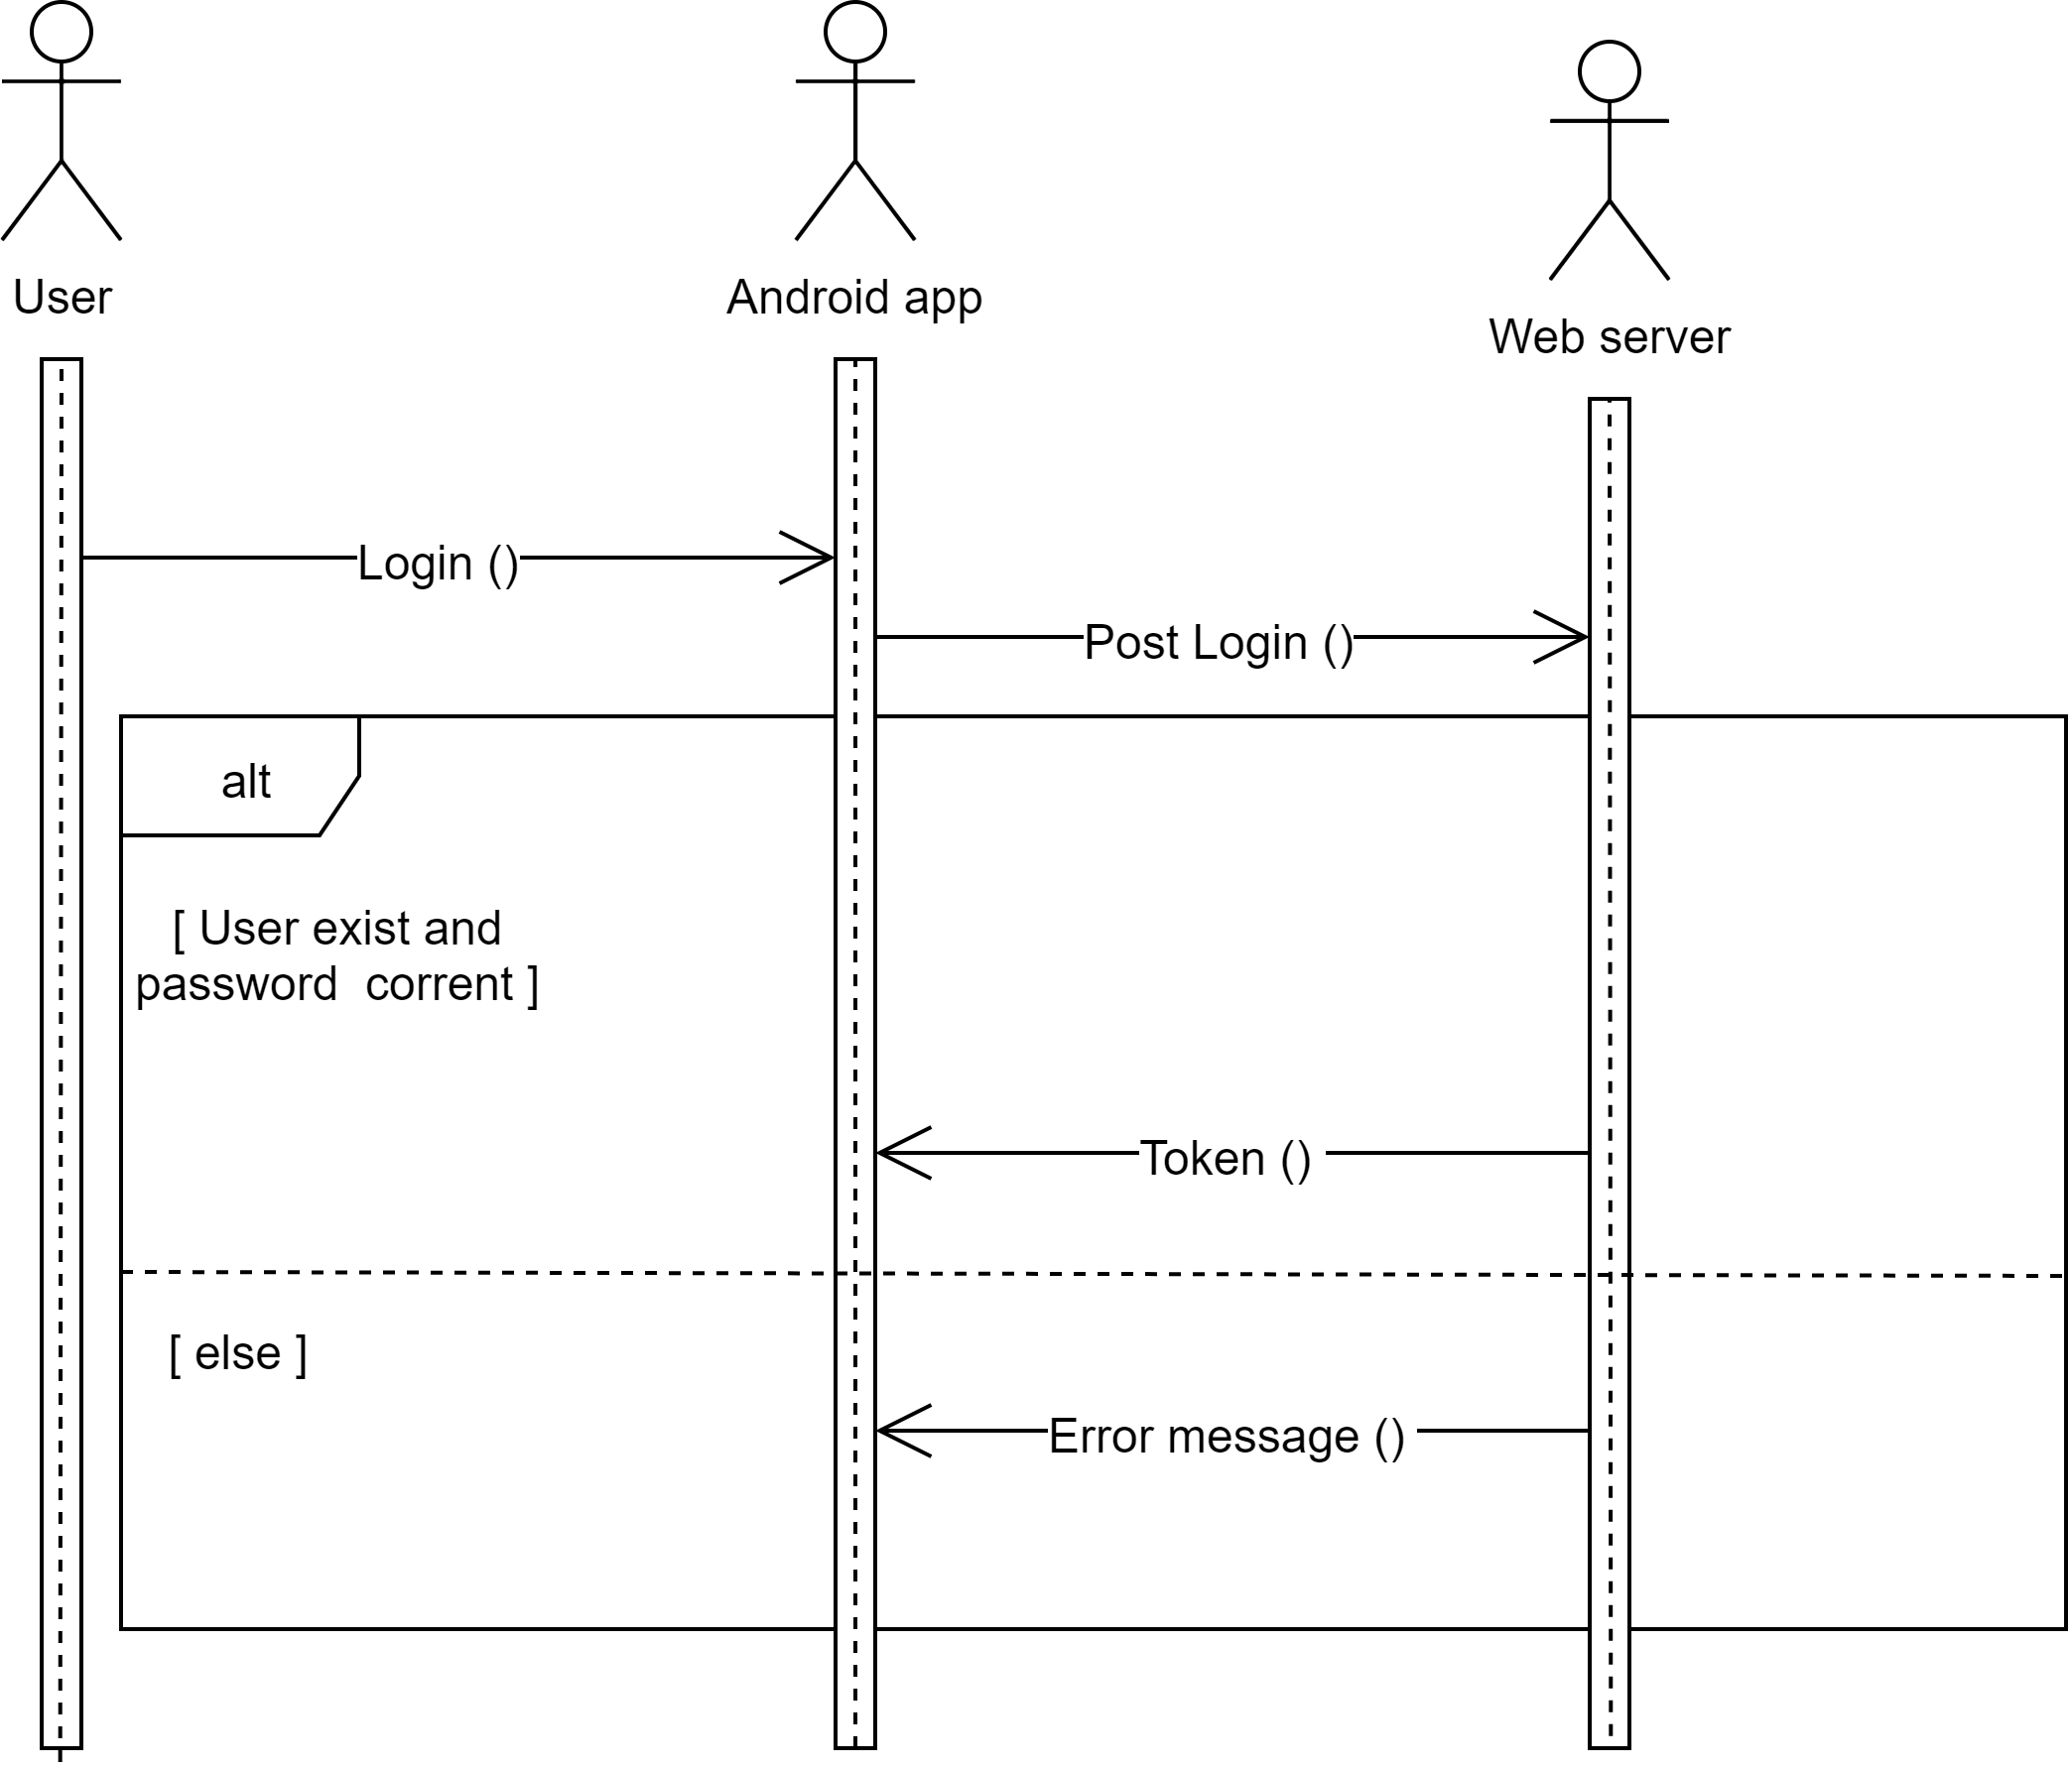
\includegraphics[width=\linewidth]{img/sequence_user_login.png}
					\caption{sequence diagram: User login or register}
					\label{user_login}
				\end{figure}
			
				\newpage\hspace*{-6mm}\boldcolor{User adds new raspberry pi}
				\newline\textbf{Sequence diagram:} \textit{Figure \ref{user_rp}}
				\newline\textbf{Goal:} to add a raspberry pi to the system
				\newline\textbf{Actors:} Android app, Web server.
				\newline\textbf{Precondition:} user logged in.
				\newline\textbf{Primary Scenario:}	
				\begin{enumerate}[label*=\arabic*.]
					\item user clicks on add new raspberry pi button.
					\item android app opens camera for the user to scan the QR code on the raspberry pi.
					\item once the code is scanned, the android app POST the raspberry pi id to the server's endpoint \code{/raspberry}.
				\end{enumerate}
				\textbf{Variant:}\newline
				\hspace*{5mm}*. user might exit android app. \\
				\hspace*{5mm}2.A. user might close camera or scan incorrect item. \\
				\hspace*{5mm}3.A. android app might fail to connect to the internet \\
				\begin{figure}[H]
					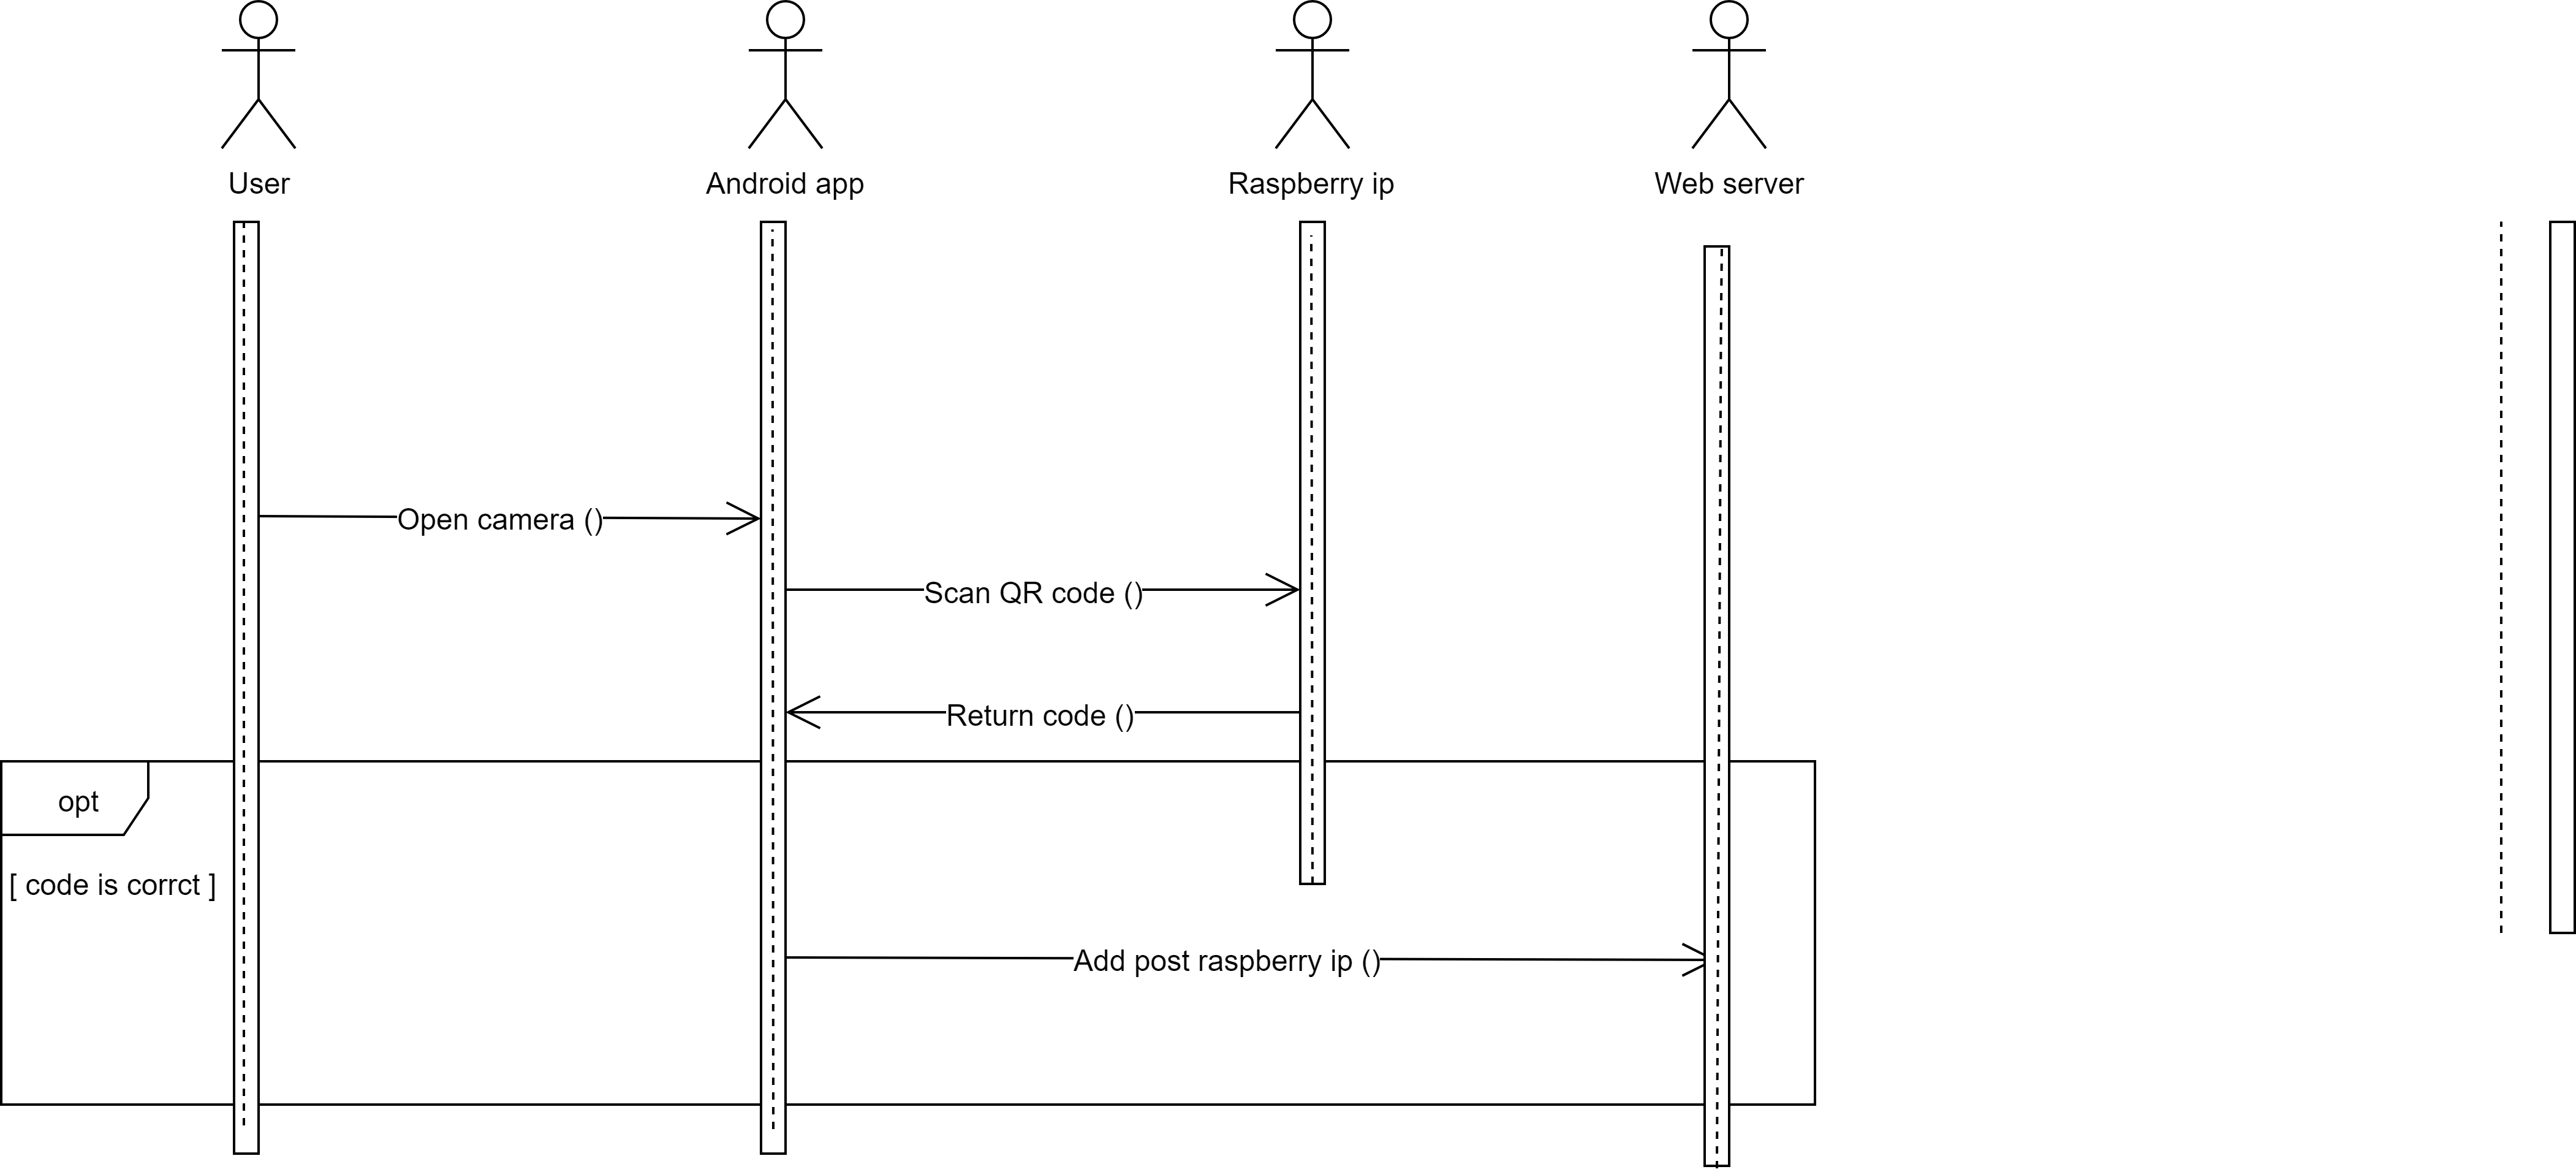
\includegraphics[width=\linewidth]{img/sequence_user_rp.png}
					\caption{sequence diagram: User adds new raspberry pi}
					\label{user_rp}
				\end{figure}
			
				\newpage\hspace*{-6mm}\boldcolor{User removes raspberry pi}
				\newline\textbf{Sequence diagram:} \textit{Figure \ref{user_rp_rm}}
				\newline\textbf{Goal:} to remove a raspberry pi from the system.
				\newline\textbf{Actors:} Android app, Web server.
				\newline\textbf{Precondition:} user logged in.
				\newline\textbf{Primary Scenario:}	
				\begin{enumerate}[label*=\arabic*.]
					\item user clicks on delete raspberry pi.
					\item Android client requests URL \code{/raspberry/\{id\}} with HTTP method \textit{DELETE} where\textit{\{id\}} is the raspberry pi selected id. 
					\item webserver receives requests and deletes the raspberry pi from user.
				\end{enumerate}
				\textbf{Variant:}\newline
				\hspace*{5mm}*. user might exit android app. \\
				\hspace*{5mm}2.A. android app might fail to connect to the internet \\
				\begin{figure}[H]
					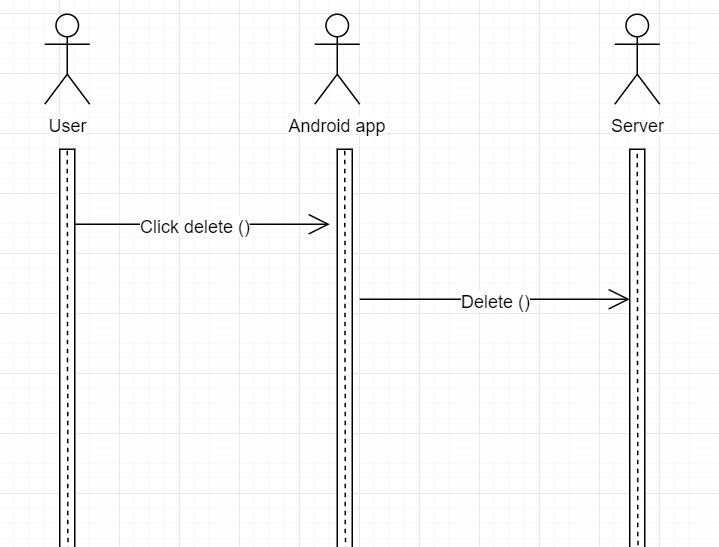
\includegraphics[width=\linewidth]{img/sequence_user_rp_rm.png}
					\caption{sequence diagram: User removes raspberry pi}
					\label{user_rp_rm}
				\end{figure}
				%%
				\newpage\hspace*{-6mm}\boldcolor{Android app gets hardware list}
				\newline\textbf{Sequence diagram:} \textit{Figure \ref{android_hw}}
				\newline\textbf{Goal:} to get all hardware in the system from webserver.
				\newline\textbf{Actors:} Android app, Web server.
				\newline\textbf{Precondition:} user logged in successfully
				\newline\textbf{Primary Scenario:}	
				\begin{enumerate}[label*=\arabic*.]
					\item user clicks on a raspberry pi.
					\item android app calls the webserver endpoint \code{/hardware}
					\item webserver fetches data from database using \code{hardware.index()}
					\item webserver responses to request with an array of hardwares in the response's body
					\item Android display this array to user in UI.
				\end{enumerate}
				\textbf{Variant:}\newline
				\hspace*{5mm}*. user might exit android app. \\
				\hspace*{5mm}1.A. android app might fail to connect to the internet \\
				\begin{figure}[H]
					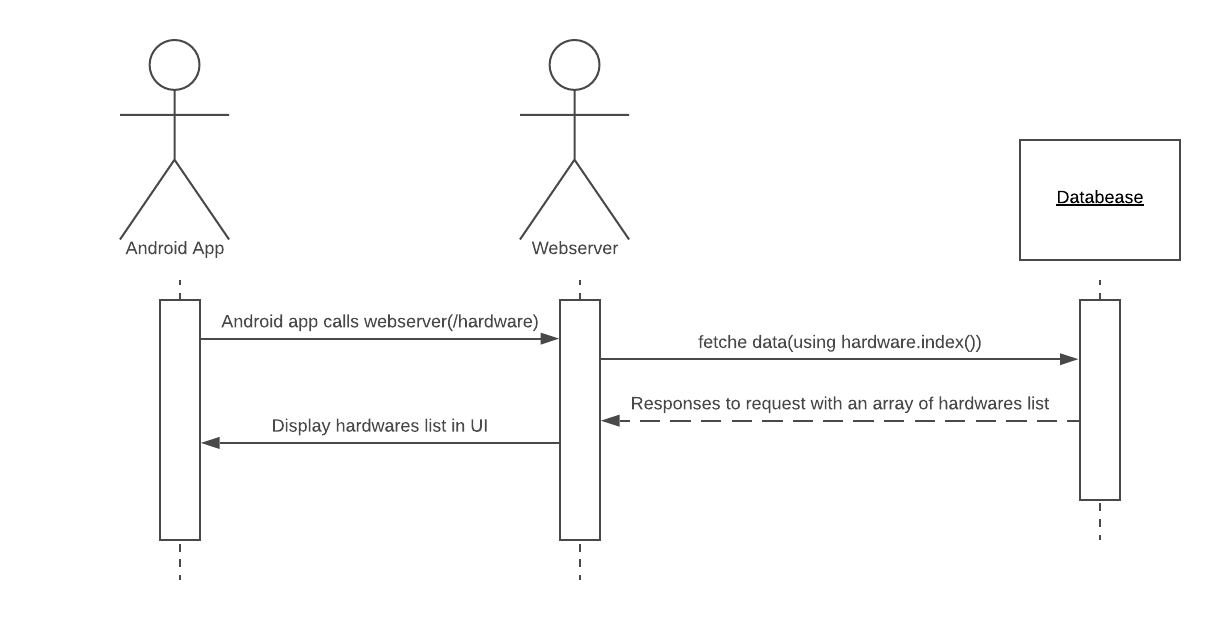
\includegraphics[width=\linewidth]{img/sequence_android_hw.png}
					\caption{sequence diagram: Android app gets hardware list}
					\label{android_hw}
				\end{figure}
				\newpage\hspace*{-6mm}\boldcolor{Android app gets command list}
				\newline\textbf{Sequence diagram:} \textit{Figure \ref{android_command_list}}
				\newline\textbf{Goal:} to get all commands in the system related to selected hardware.
				\newline\textbf{Actors:} Android app, Web server.
				\newline\textbf{Precondition:} android app gets hardware list
				\newline\textbf{Primary Scenario:}	
				\begin{enumerate}[label*=\arabic*.]
					\item user selects hardware from UI.
					\item android app calls the webserver endpoint \code{/hardware/\{hardwareId\}/command}, where \textit{hardwareId} is the id of the hardware the user selected.
					\item webserver fetches data from database using \code{command.indexByHardwareId(\{hardwareId\})}
					\item webserver responds to request with an array of commands in the response's body
				\end{enumerate}
				\textbf{Variant:}\newline
				\hspace*{5mm}*. user might exit android app. \\
				\hspace*{5mm}2.A. android app might fail to connect to the internet \\
				\begin{figure}[H]
					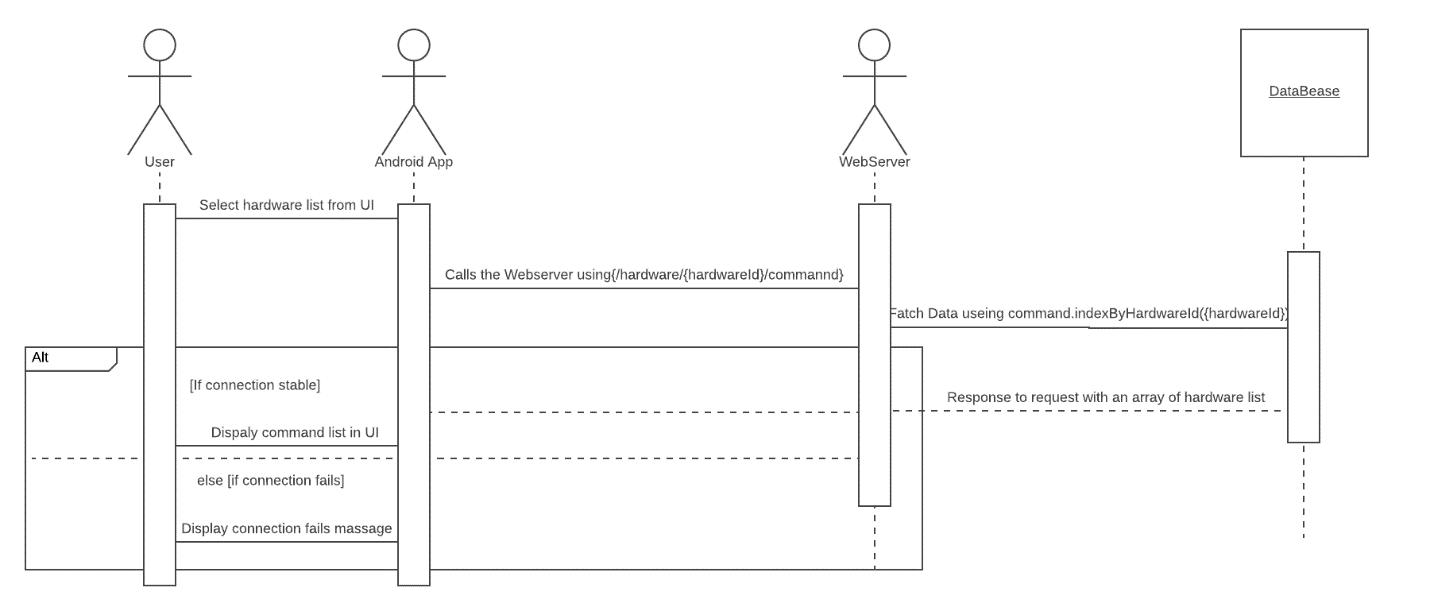
\includegraphics[width=\linewidth]{img/sequence_android_command_list.png}
					\caption{sequence diagram: Android app gets command list}
					\label{android_command_list}
				\end{figure}
				\newpage\hspace*{-6mm}\boldcolor{Android app deletes a scheduled command}
				\newline\textbf{Sequence diagram:} \textit{Figure \ref{android_del}}
				\newline\textbf{Goal:} to delete a scheduled command from webserver related to selected hardware.
				\newline\textbf{Actors:} User, Android app, Web server
				\newline\textbf{Precondition:} android app gets all scheduled command.
				\newline\textbf{Primary Scenario:}	
				\begin{enumerate}[label*=\arabic*.]
					\item User clicks on delete a scheduled command.
					\item Android client requests URL \code{/command/\{id\}} with HTTP method \textit{DELETE} where\textit{\{id\}} is the command selected id. 
					\item  webserver receives requests and deletes the command.
				\end{enumerate}
				\textbf{Variant:}\newline
				\hspace*{5mm}1.A. user might not have a schedule command. \\
				\hspace*{5mm}2.A. android app might fail to connect to the internet \\
				\begin{figure}[H]
					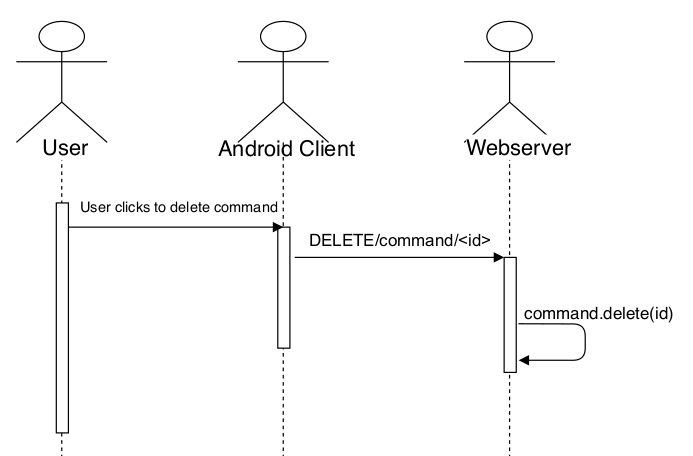
\includegraphics[width=\linewidth]{img/sequence_android_delete.png}
					\caption{sequence diagram: Android app deletes a scheduled command}
					\label{android_del}
				\end{figure}
				\newpage\hspace*{-6mm}\boldcolor{Android app edits a scheduled command}
				\newline\textbf{Sequence diagram:} \textit{Figure \ref{android_edit}}
				\newline\textbf{Goal:} to edit a scheduled command from webserver related to selected hardware. 
				\newline\textbf{Actors:} User, Android app, Web server
				\newline\textbf{Precondition:} android app gets all scheduled command.
				\newline\textbf{Primary Scenario:}	
				\begin{enumerate}[label*=\arabic*.]
					\item User clicks on editing a scheduled command.
					\item Android client requests URL \code{/command/\{id\}} with HTTP method \textit{PUT} where\textit{\{id\}} is the command selected id. 
					\item  webserver receives requests and edits the command.
				\end{enumerate}
				\textbf{Variant:}\newline
				\hspace*{5mm}1.A. user might not have a schedule command. \\
				\hspace*{5mm}2.A. android app might fail to connect to the internet \\
				\begin{figure}[H]
					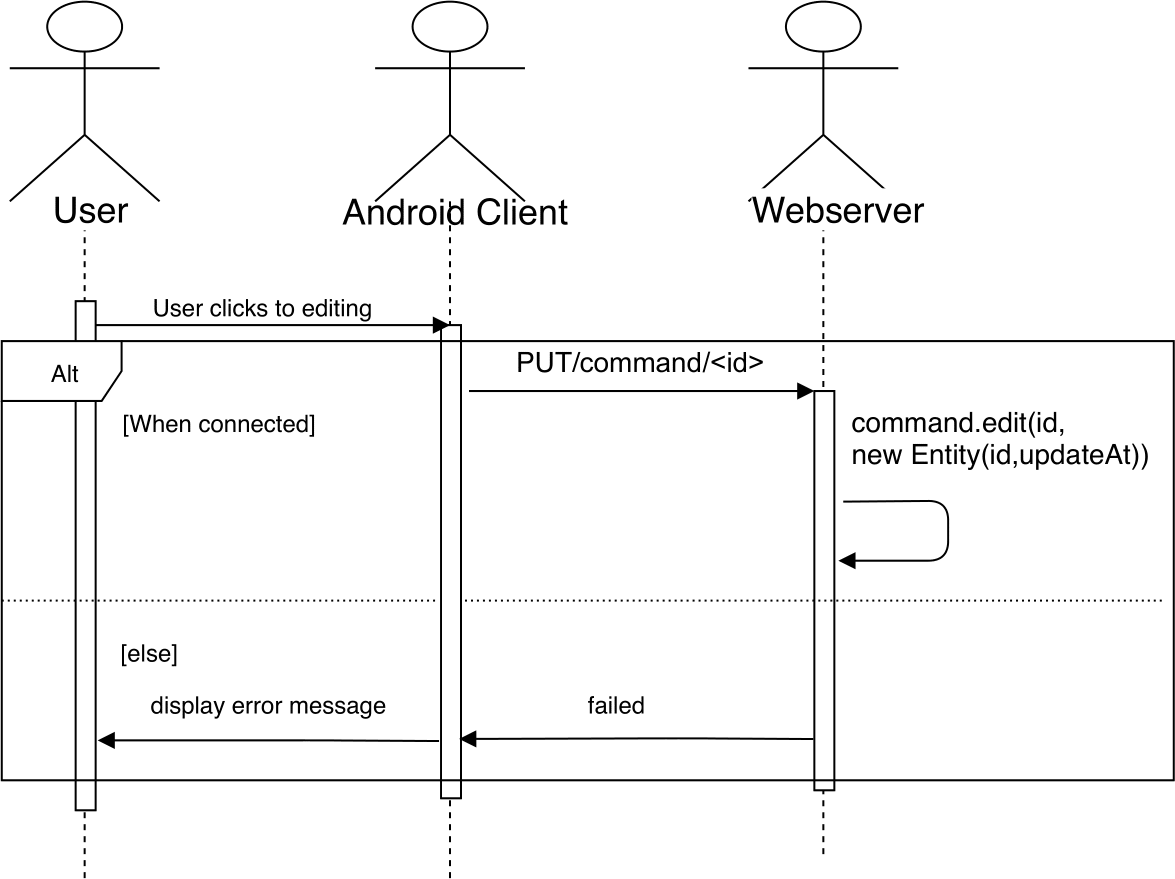
\includegraphics[width=\linewidth]{img/sequence_android_edit.png}
					\caption{sequence diagram: Android app edits a scheduled command}
					\label{android_edit}
				\end{figure}
				\newpage\hspace*{-6mm}\boldcolor{Android app adds a new command}
				\newline\textbf{Sequence diagram:} \textit{Figure \ref{android_add}}
				\newline\textbf{Goal:} to add a new command to webserver.
				\newline\textbf{Actors:} User, Android app, Web server
				\newline\textbf{Precondition:} android app gets all hardwares and user chooses the hardware to add command to.
				\newline\textbf{Primary Scenario:}	
				\begin{enumerate}[label*=\arabic*.]
					\item User clicks on adding  a new command.
					\item activity appears taking the new command attributes, such as schedule or configuration.
					\item Android client requests URL \code{/command} with HTTP method \textit{POST}.
					\item  webserver receives requests and adds the command.
				\end{enumerate}
				\textbf{Variant:}\newline
				\hspace*{5mm}*. internet might disconnect\\
				\begin{figure}[H]
					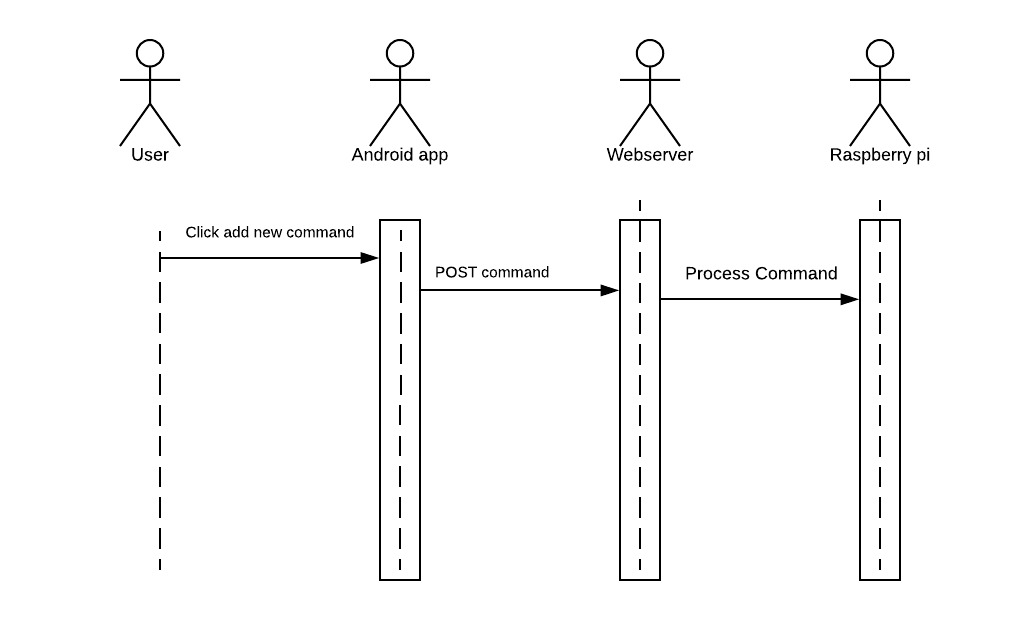
\includegraphics[width=\linewidth]{img/sequence_android_add.jpg}
					\caption{sequence diagram: Android app adds a new command}
					\label{android_add}
				\end{figure}
				\newpage\hspace*{-6mm}\boldcolor{Android app gets responses}
				\newline\textbf{Sequence diagram:} \textit{Figure \ref{android_response}}
				\newline\textbf{Goal:} to get the result of the command execution to the user as a notification
				\newline\textbf{Actors:} Android app, Web server
				\newline\textbf{Precondition:} None
				\newline\textbf{Primary Scenario:}	
				\begin{enumerate}[label*=\arabic*.]
					\item Android client requests URL \code{/response} every 5 or 10 minutes.
					\item if responses exist, android app shows it to user as a push notification.
				\end{enumerate}
				\textbf{Variant:}\newline
				\hspace*{5mm}*. internet might disconnect\\
				\begin{figure}[H]
					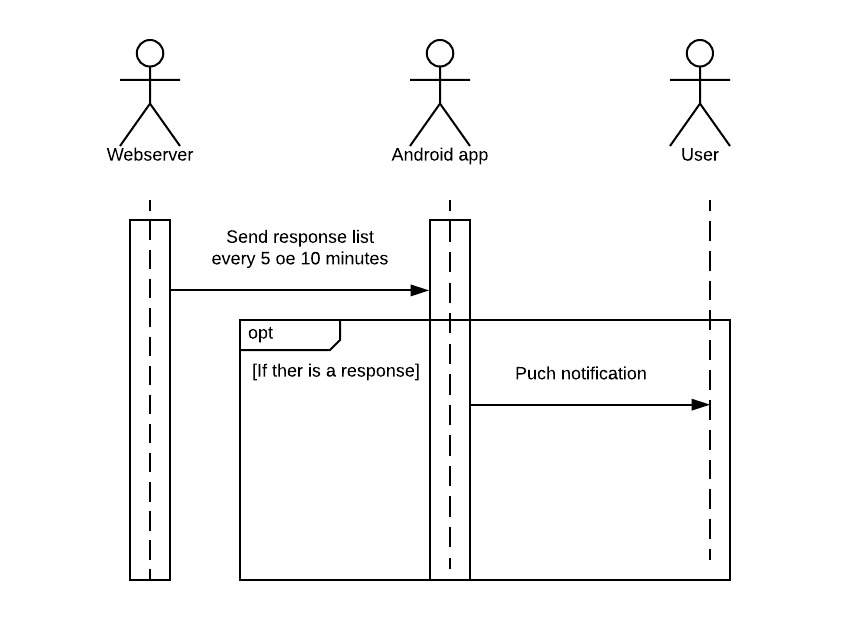
\includegraphics[width=\linewidth]{img/sequence_android_response.jpg}
					\caption{sequence diagram: Android app gets responses}
					\label{android_response}
				\end{figure}
				\newpage\hspace*{-6mm}\boldcolor{Raspberry pi gets command list}
				\newline\textbf{Sequence diagram:} \textit{Figure \ref{rp_command_list}}
				\newline\textbf{Goal:} to get all commands in the system.
				\newline\textbf{Actors:} Raspberry pi, Web server.
				\newline\textbf{Precondition:} None
				\newline\textbf{Primary Scenario:}	
				\begin{enumerate}[label*=\arabic*.]
					\item Raspberry pi calls the webserver endpoint \code{/command} to get all the commands
					\item webserver fetches data from database using \code{command.index()}
					\item webserver responds to request with an array of commands in the response's body
				\end{enumerate}
				\textbf{Variant:}\newline
				\hspace*{5mm}*. raspberry pi might fail to connect to the internet \\
				\begin{figure}[H]
					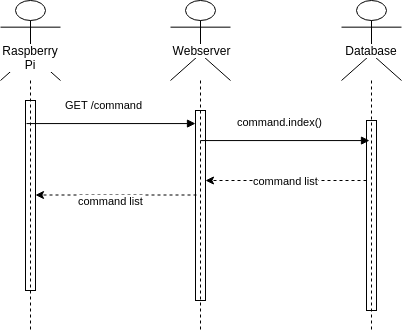
\includegraphics[width=\linewidth]{img/sequece_rp_command.png}
					\caption{sequence diagram: Raspberry pi gets commands from server}					
					\label{rp_command_list}
				\end{figure}
				\newpage\hspace*{-6mm}\boldcolor{Raspberry pi updates local queue}
				\newline\textbf{Sequence diagram:} \textit{Figure \ref{rp_queue}}
				\newline\textbf{Goal:} to updates local queue.
				\newline\textbf{Actors:} Raspberry pi.
				\newline\textbf{Precondition:} raspberry pi got  command List from web server.
				\newline\textbf{Primary Scenario:}	
				\begin{enumerate}[label*=\arabic*.]
					\item Raspberry pi gets a command from list.
					\item If command is immediate,i.e. has no schedule, the execution time for the processed command will be the time the command was created - accessed using  \code{command.getUpdateAt()}-.
					\item else -meaning command has a schedule- and today is part of the schedule days, add to queue with execution Time set to today at the schedule's time.
					\item order queue by execution Time
				\end{enumerate}
				\textbf{Variant:}\newline
				\hspace*{5mm}3.A. if today is not part of the days, discard command \\
				\begin{figure}[H]
					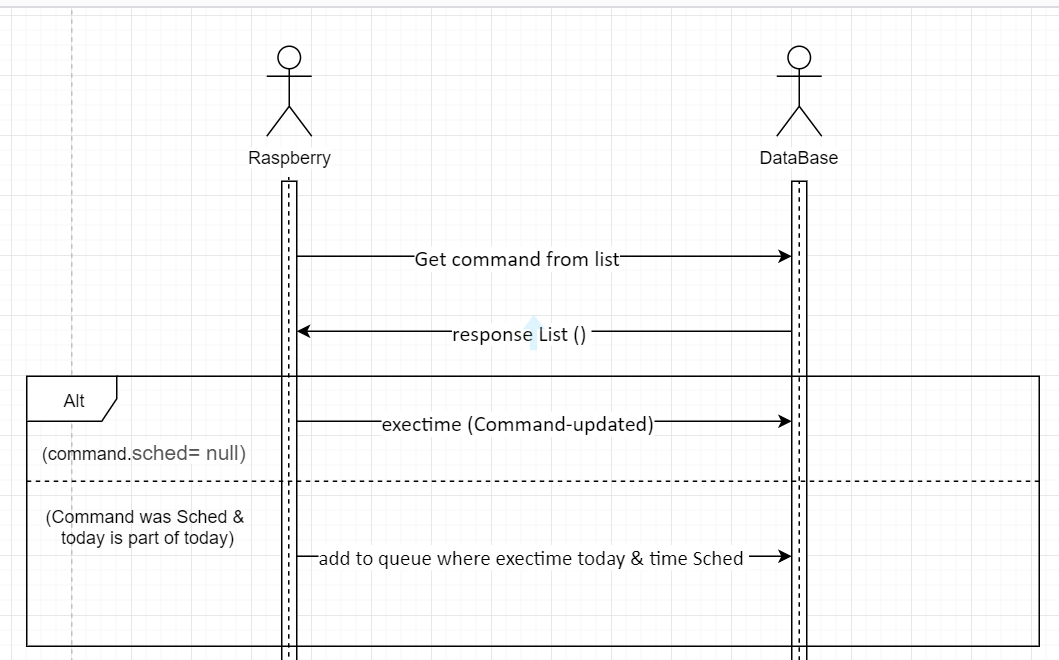
\includegraphics[width=\linewidth]{img/sequence_queue.png}
					\caption{sequence diagram: Raspberry pi updates local queue}					\label{rp_queue}
				\end{figure}
				\newpage\hspace*{-6mm}\boldcolor{Raspberry pi executes commands}
				\newline\textbf{Sequence diagram:} \textit{Figure \ref{rp_execute}}
				\newline\textbf{Goal:} to execute commands saved in the local queue on a timely fashion.
				\newline\textbf{Actors:} Raspberry Pi.	
				\newline\textbf{Precondition:} raspberry pi got the commands from webserver, updated local database.
				\newline\textbf{Primary Scenario:}	
				\begin{enumerate}[label*=\arabic*.]
					\item raspberry pi fetches first processed command saved in local queue.
					\item raspberry pi calls the function \code{EcecuteCommand()} and pass it the command as a parameter.
					\item raspberry pi look for the pin connecting the hardware and apply the desired configuration to it.
				\end{enumerate}
				\textbf{Variant:}\newline	
				\hspace*{5mm}1.A. local queue might be empty, no action is taken. \\
				\hspace*{5mm}2.A. a hardware error might happen, such as disconnected cable. \\
				\begin{figure}[H]
					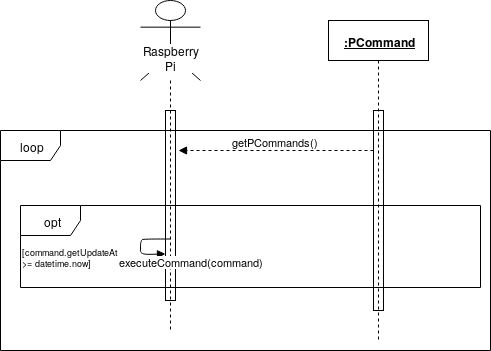
\includegraphics[width=\linewidth]{img/sequence_execute.png}
					\caption{sequence diagram: Raspberry pi executes commands}					
					\label{rp_execute}
				\end{figure}
				\newpage\hspace*{-6mm}\boldcolor{Raspberry pi submits a command response to server}
				\newline\textbf{Sequence diagram:} \textit{Figure \ref{rp_response}}
				\newline\textbf{Goal:} to submit the result of the command execution to the server by saving it as a response row.
				\newline\textbf{Actors:} Raspberry Pi, webserver.
				\newline\textbf{Precondition:} raspberry pi executed commands.
				\newline\textbf{Primary Scenario:}	
				\begin{enumerate}[label*=\arabic*.]
					\item raspberry pi determines whether the execution was successful. 
					\item raspberry pi includes a message if any.
					\item  raspberry pi requests the webserver endpoint \code{/response} with the method \textit{POST}, needed parameter are added to the request body.
					\item webserver receives request, a new row to the database response table is added and ready for the android client to read. 
				\end{enumerate}
				\textbf{Variant:}\newline	
				\hspace*{5mm}*. internet might disconnect.\\
				\begin{figure}[H]
					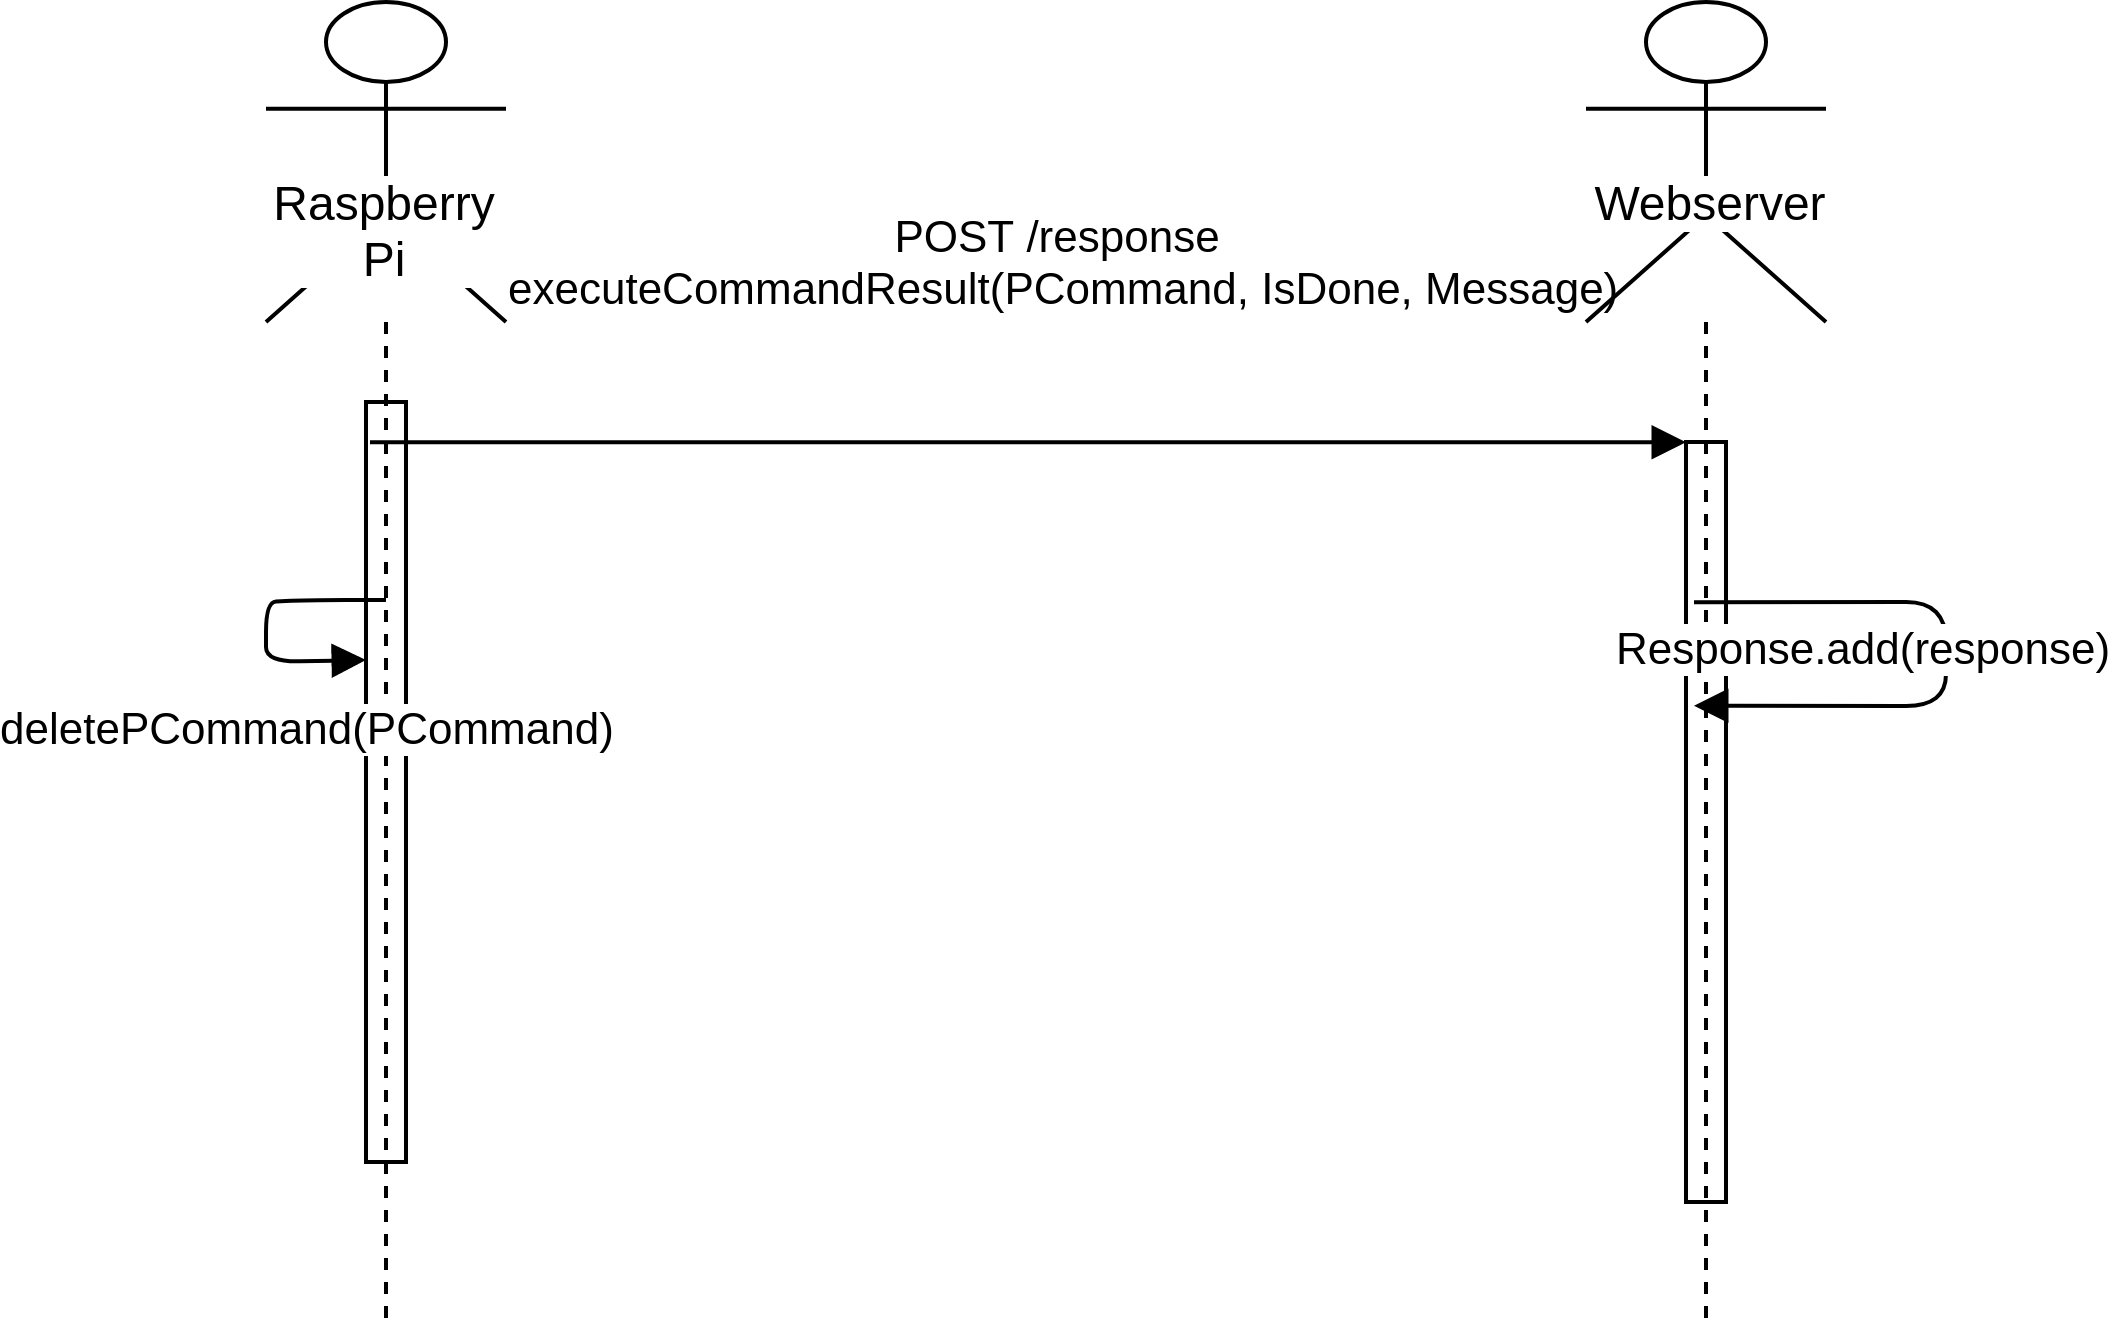
\includegraphics[width=\linewidth]{img/sequence_submit_response.png}
					\caption{sequence diagram: Raspberry pi submits a command response to server}
					\label{rp_response}
				\end{figure}
				\newpage\hspace*{-6mm}\boldcolor{Web application deletes executed immediate commands}
				\newline\textbf{Sequence diagram:} \textit{Figure \ref{web_delete_c}}
				\newline\textbf{Goal:} to delete all executed immediate commands.
				\newline\textbf{Actors:} Web application, database.
				\newline\textbf{Precondition:} None
				\newline\textbf{Primary Scenario:}	
				\begin{enumerate}[label*=\arabic*.]
					\item Web application join between a command table and Response table from database.  
					\item  Web application will select the immediate command from database using \code{Command.scheduled=null}.
					\item Web application checks if response has been read by the user. using \code{response.isRead()} then, deletes command.
				\end{enumerate}
				\begin{figure}[H]
					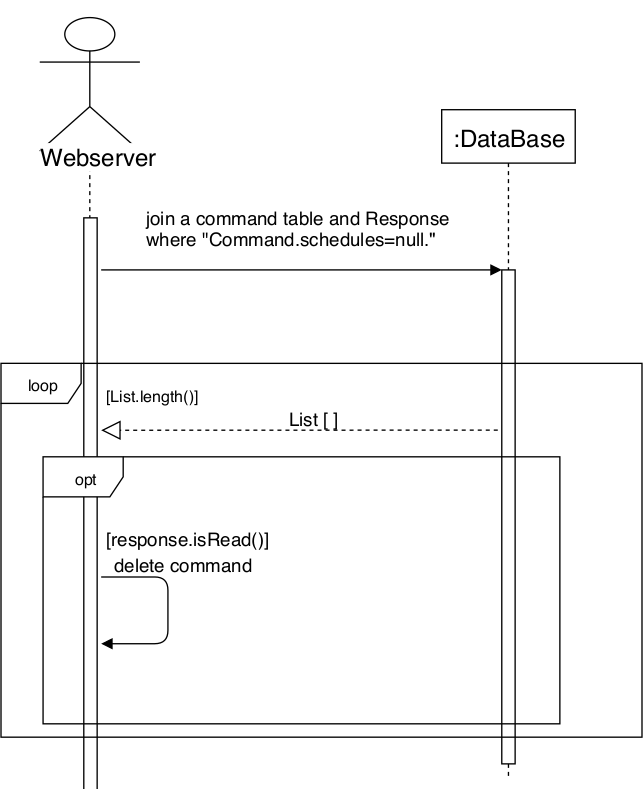
\includegraphics[width=\linewidth]{img/sequence_w_delete_c.png}
					\caption{sequence diagram: Web application deletes executed immediate commands}
					\label{web_delete_c}
				\end{figure}
				\newpage\hspace*{-6mm}\boldcolor{Web application deletes read responses}
				\newline\textbf{Sequence diagram:} \textit{Figure \ref{web_delete_r}}
				\newline\textbf{Goal:} to delete all read responses.
				\newline\textbf{Actors:} Web application, database.
				\newline\textbf{Precondition:} None
				\newline\textbf{Primary Scenario:}	
				\begin{enumerate}[label*=\arabic*.]
					\item Web application fetches responses from database 
					\item if response has been read by the user, delete it.
				\end{enumerate}	
				\begin{figure}[H]
					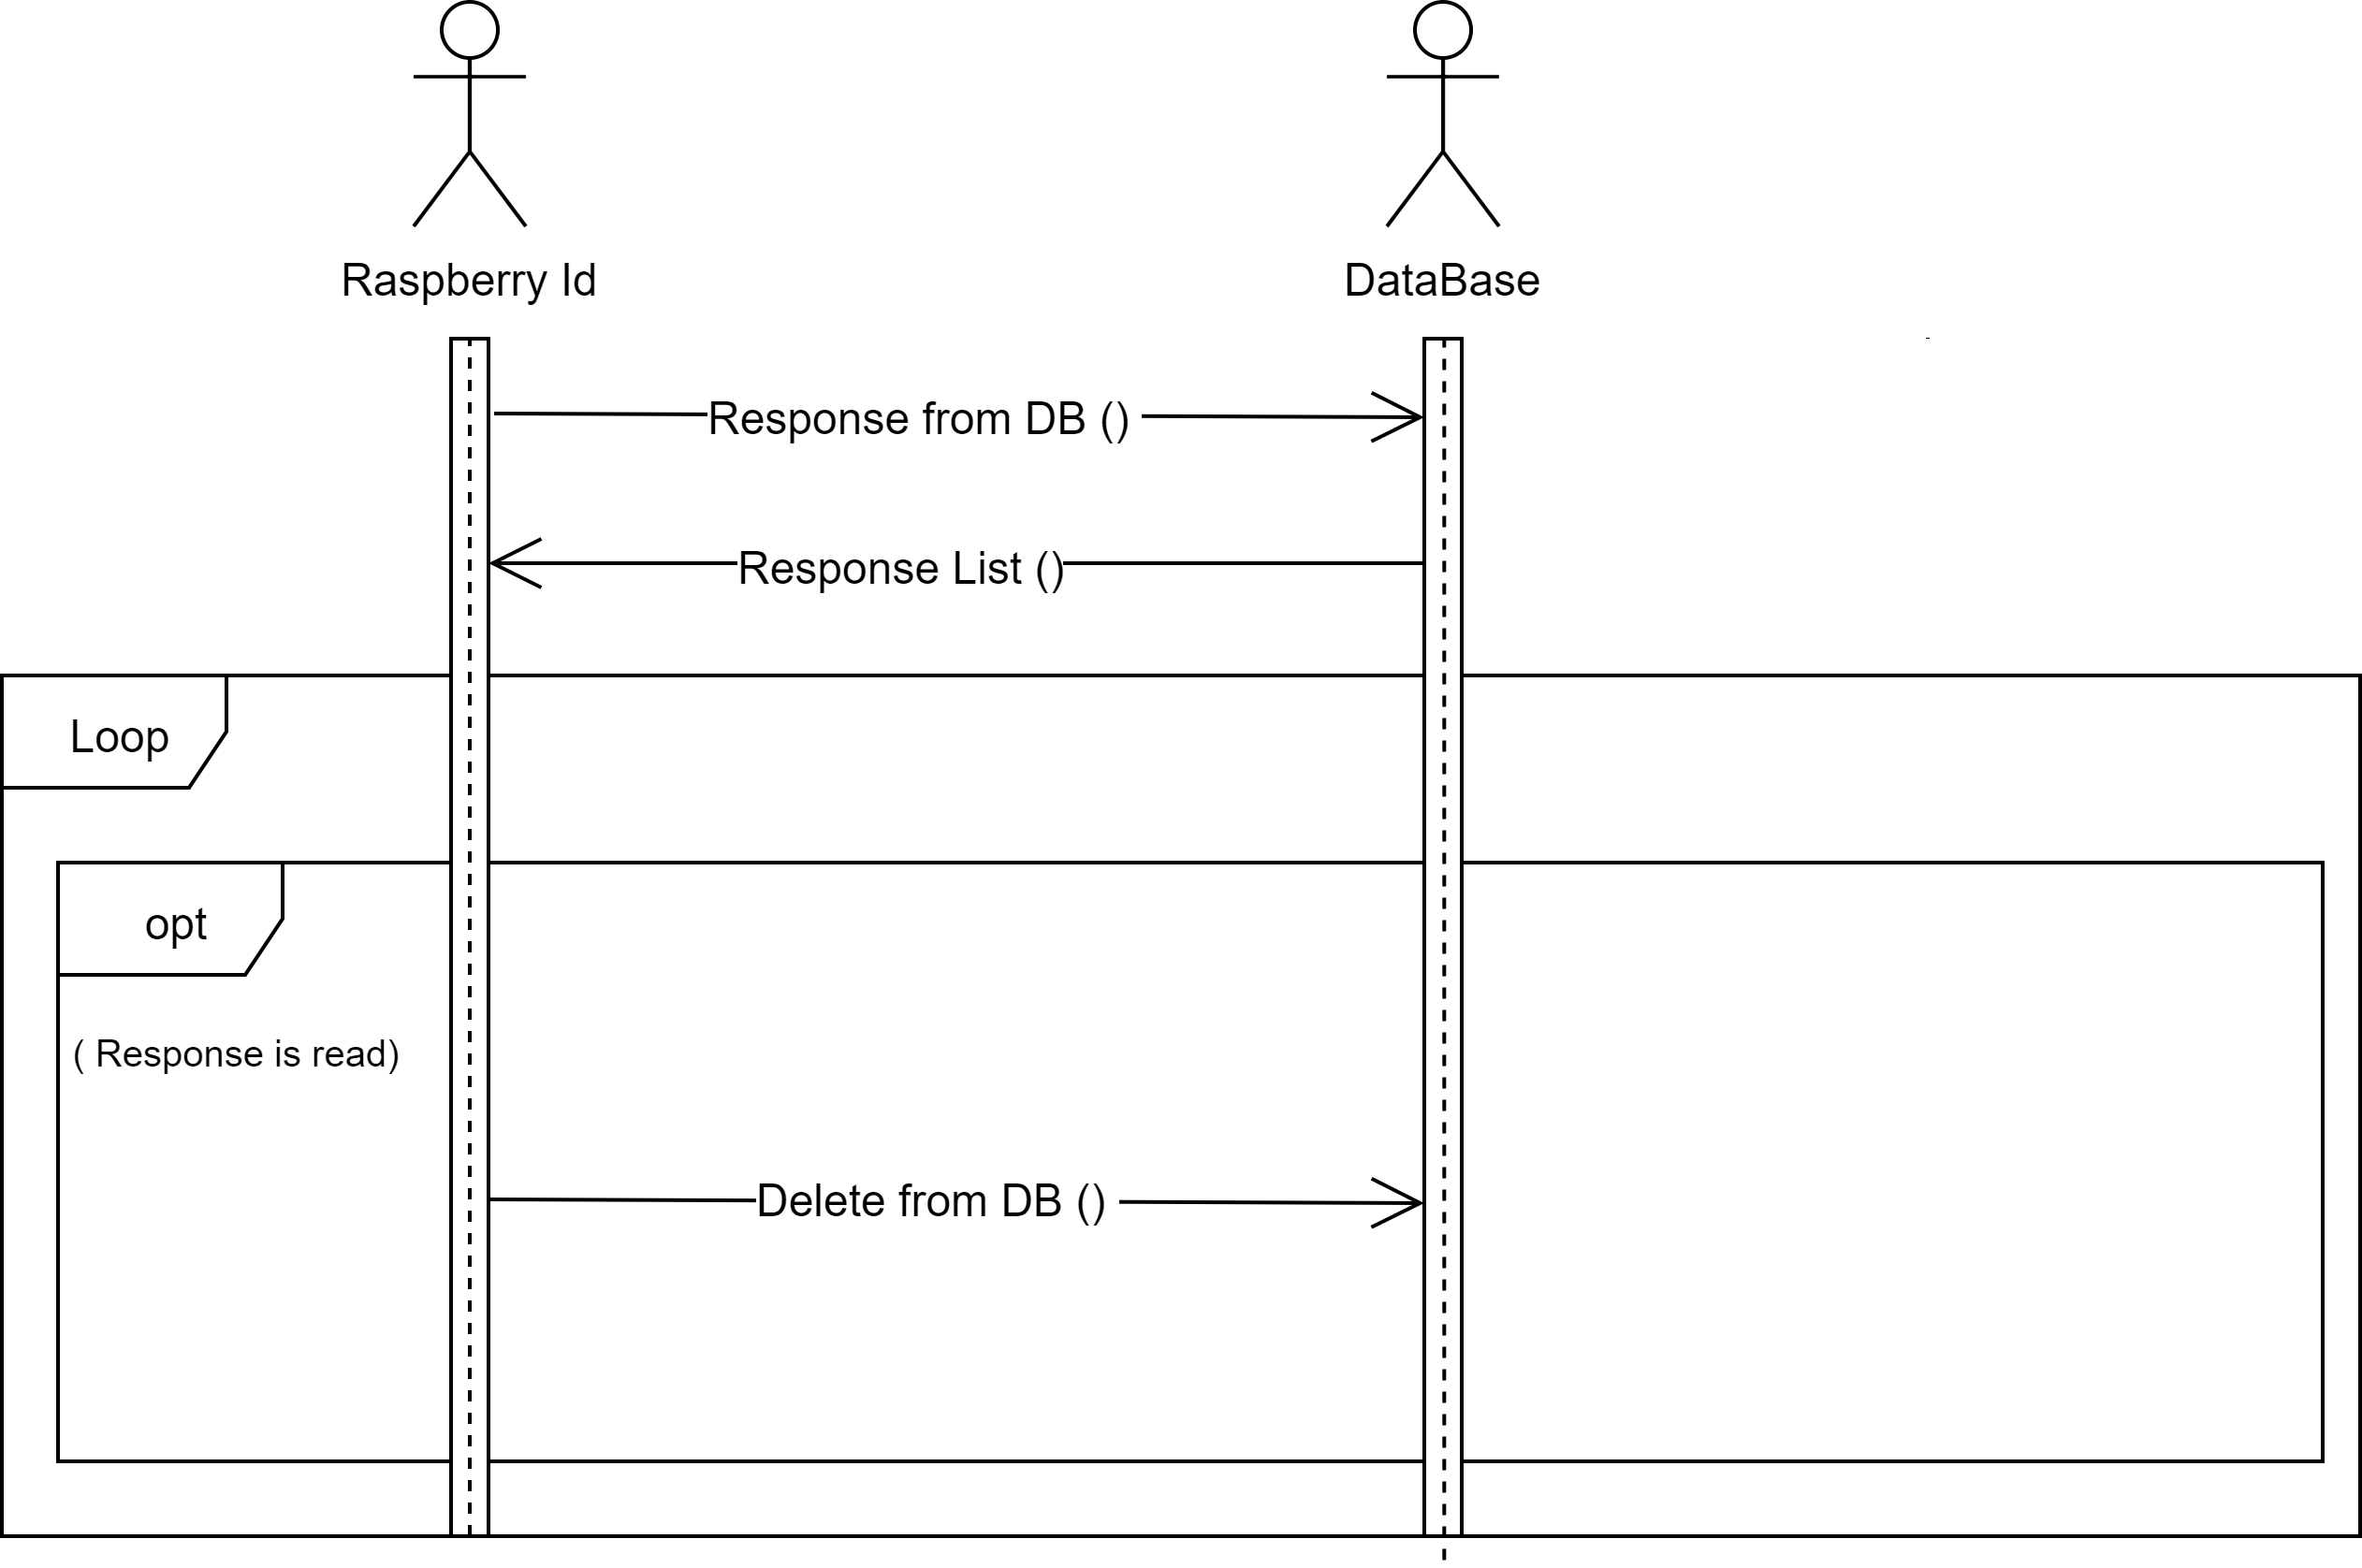
\includegraphics[width=\linewidth]{img/sequence_web_del_r.png}
					\caption{sequence diagram: Web application deletes responses}
					\label{web_delete_r}
				\end{figure}
				\newpage\subsubsection{Flowchart Diagram}
				\paragraph{} Figure \ref{fig:ig:flow_android} shows the flow chart for the android app, and figure \ref{fig:ig:flow_rasp} shows the raspberry pi's flowchart.
				\begin{itemize}
					\item \boldcolor{Raspberry pi}: Every 30 seconds, raspberry first requests command list from the server, the web application then fetches the list from the database and returns it. Raspberry pi updates the local queue with them. It then checks the first command in the queue, if it was due it gets executed and post the response to the server. After execution,  it checks the first in queue again.
					\item \boldcolor{Android app}: when android app is first opened, it requests hardware list from the webserver. After the web app fetches the hardware list from the database, it returns it to the android app, which displays the hardwares to the user. If the user clicks in a hardware, a new activity is opened containing the hardware information and the command list for that hardware. The user then can do 3 things: 
					\begin{enumerate}
						\item Edit a certain command: android request PUT to the command chosen from the server.
						\item Delete a certain command: android request DELETE to the command chosen from the server.
						\item Add a new command: android shows a new activity prompting the user for the command information, then it requests POST command to the server. 
					\end{enumerate}
					Regardless of the choice, the web app then process the request.
					\item \boldcolor{Android app back work}: each 5 or 10 minutes, android requests the responses from the webserver. When there is a response to be read, it shows it to the user as a push notification.
					\item \boldcolor{Web app}: when a command has no schedule and it was executed, the web app immediately deletes it from the database. Web app also deletes any read response.
				\end{itemize}
				\begin{figure}[H]
					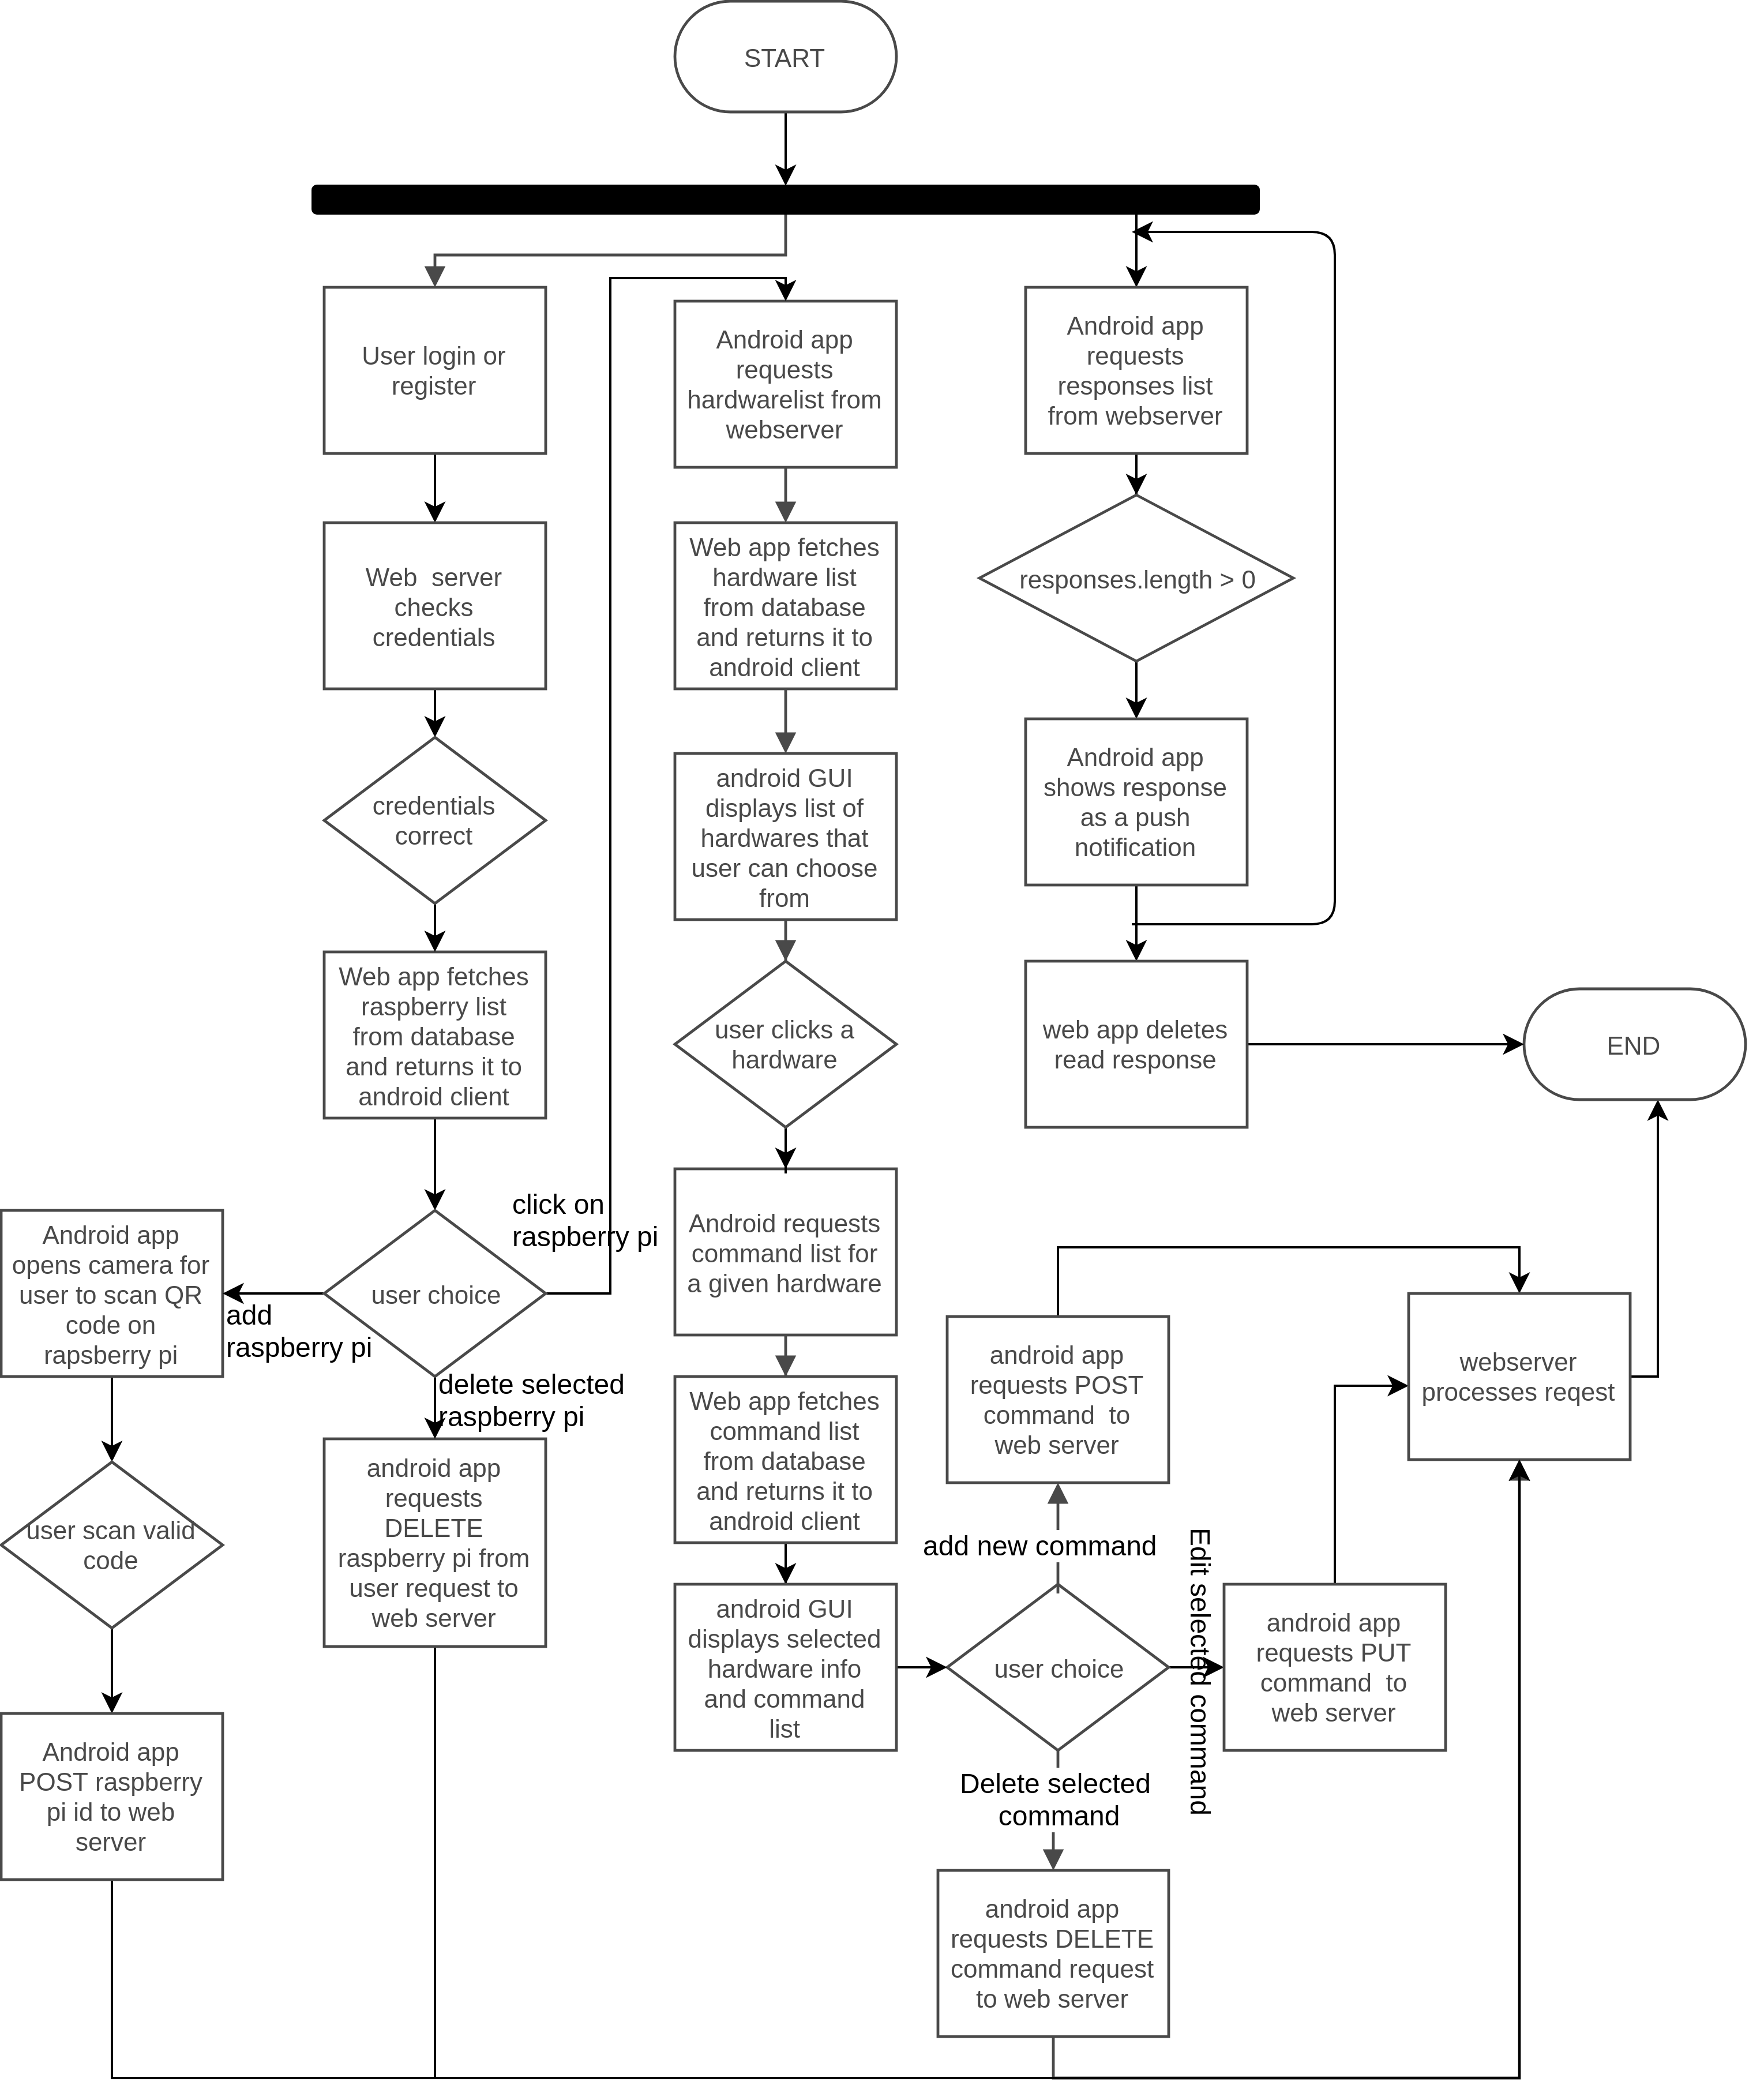
\includegraphics[width=\linewidth]{img/flowchart_android.png}
					\caption{Flow chart - Android app}
					\label{fig:ig:flow_android}
				\end{figure}
				\begin{figure}[H]
					\centering
					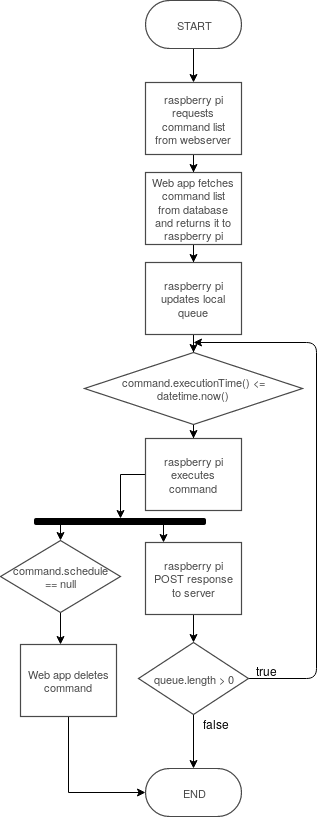
\includegraphics[width=.65\linewidth]{img/flowchart_raspberry.png}
					\caption{Flow chart - Raspberry pi}
					\label{fig:ig:flow_rasp}
				\end{figure}
				\newpage\subsubsection{Entity Relationship Diagram}
					\paragraph{} In our system, there are two databases: the \textit{system database} stored in the web server, and \textit{the queue}, a local database for the raspberry pi. To make understanding the databases' easier, we represented it using entity relationship diagram. It is a graphical representation that demonstrates the relationship between concept, people, places, objects or events inside a system. The main components are the entities, relationship and cardinality. Entities are concepts or object that need their data stored. Cardinality defines that relationship in terms of numbers\cite{erd}.
				
				\begin{itemize}
					\item \boldcolor{System database}: This database is the main database. It will be stored in the web server and gets accessed by the android client and the raspberry pi. There are 7 main entities: 
					\begin{enumerate}
						\item \textbf{User:} to manage access, a user entity is essential. IT will store the user credentials. 
						\item \textbf{RaspberryPi:} Here, the data for each physical raspberry pi is saved. Each user can have many raspberry pis and each  raspberry can belong to multiple people.
						\item \textbf{Hardware:} it will store information related to the physical components connected to a raspberry pi. Such as LED lights, linear solenoid or an infra-red controller.  
						\item \textbf{Configuration:} hardwares can have different states. For example, a LED light could be on or off. An RGB LED can be ON on a certain color, of off. Configurations save the possible states a hardware can be in.
						\item \textbf{Command:} users can change raspberry pi's hardwares to be in a certain configuration. These commands are stored here. The users requests could either be instant, or scheduled. 
						\item \textbf{Schedule:} since commands can be scheduled, those data should be saved here. The user can choose the days and time a command fires.
						\item \textbf{Response:} when raspberry pi finish executing a command, it issues a response.
					\end{enumerate}
					\item \boldcolor{Local Queue}: This database is stored locally in raspberry pi. After raspberry gets user commands from server, it process them and order them based on their execution time.
					\begin{enumerate}
						\item \textbf{Hardware:} similar to the server's hardware list, this entity store the hardware connected. The system database gets data related to hardware from this entity 
						\item \textbf{Configuration:} this table stores the possible configuration. When the table is edited, the server database is updated.
						\item \textbf{PCommand:} only the commands to be executed are stored here, once a command is executed, it gets deleted from the queue. This entity contains processed commands. i.e each queue stores the exact date and time a command will be executed instead of the schedule information.
					\end{enumerate}
				\end{itemize}
			
			\textit{Figure \ref{fig:erd} shows the Entity-relationship diagram.} 
					\begin{figure}[H]
						\label{fig:erd}
						\begin{subfigure}[b]{\linewidth}
							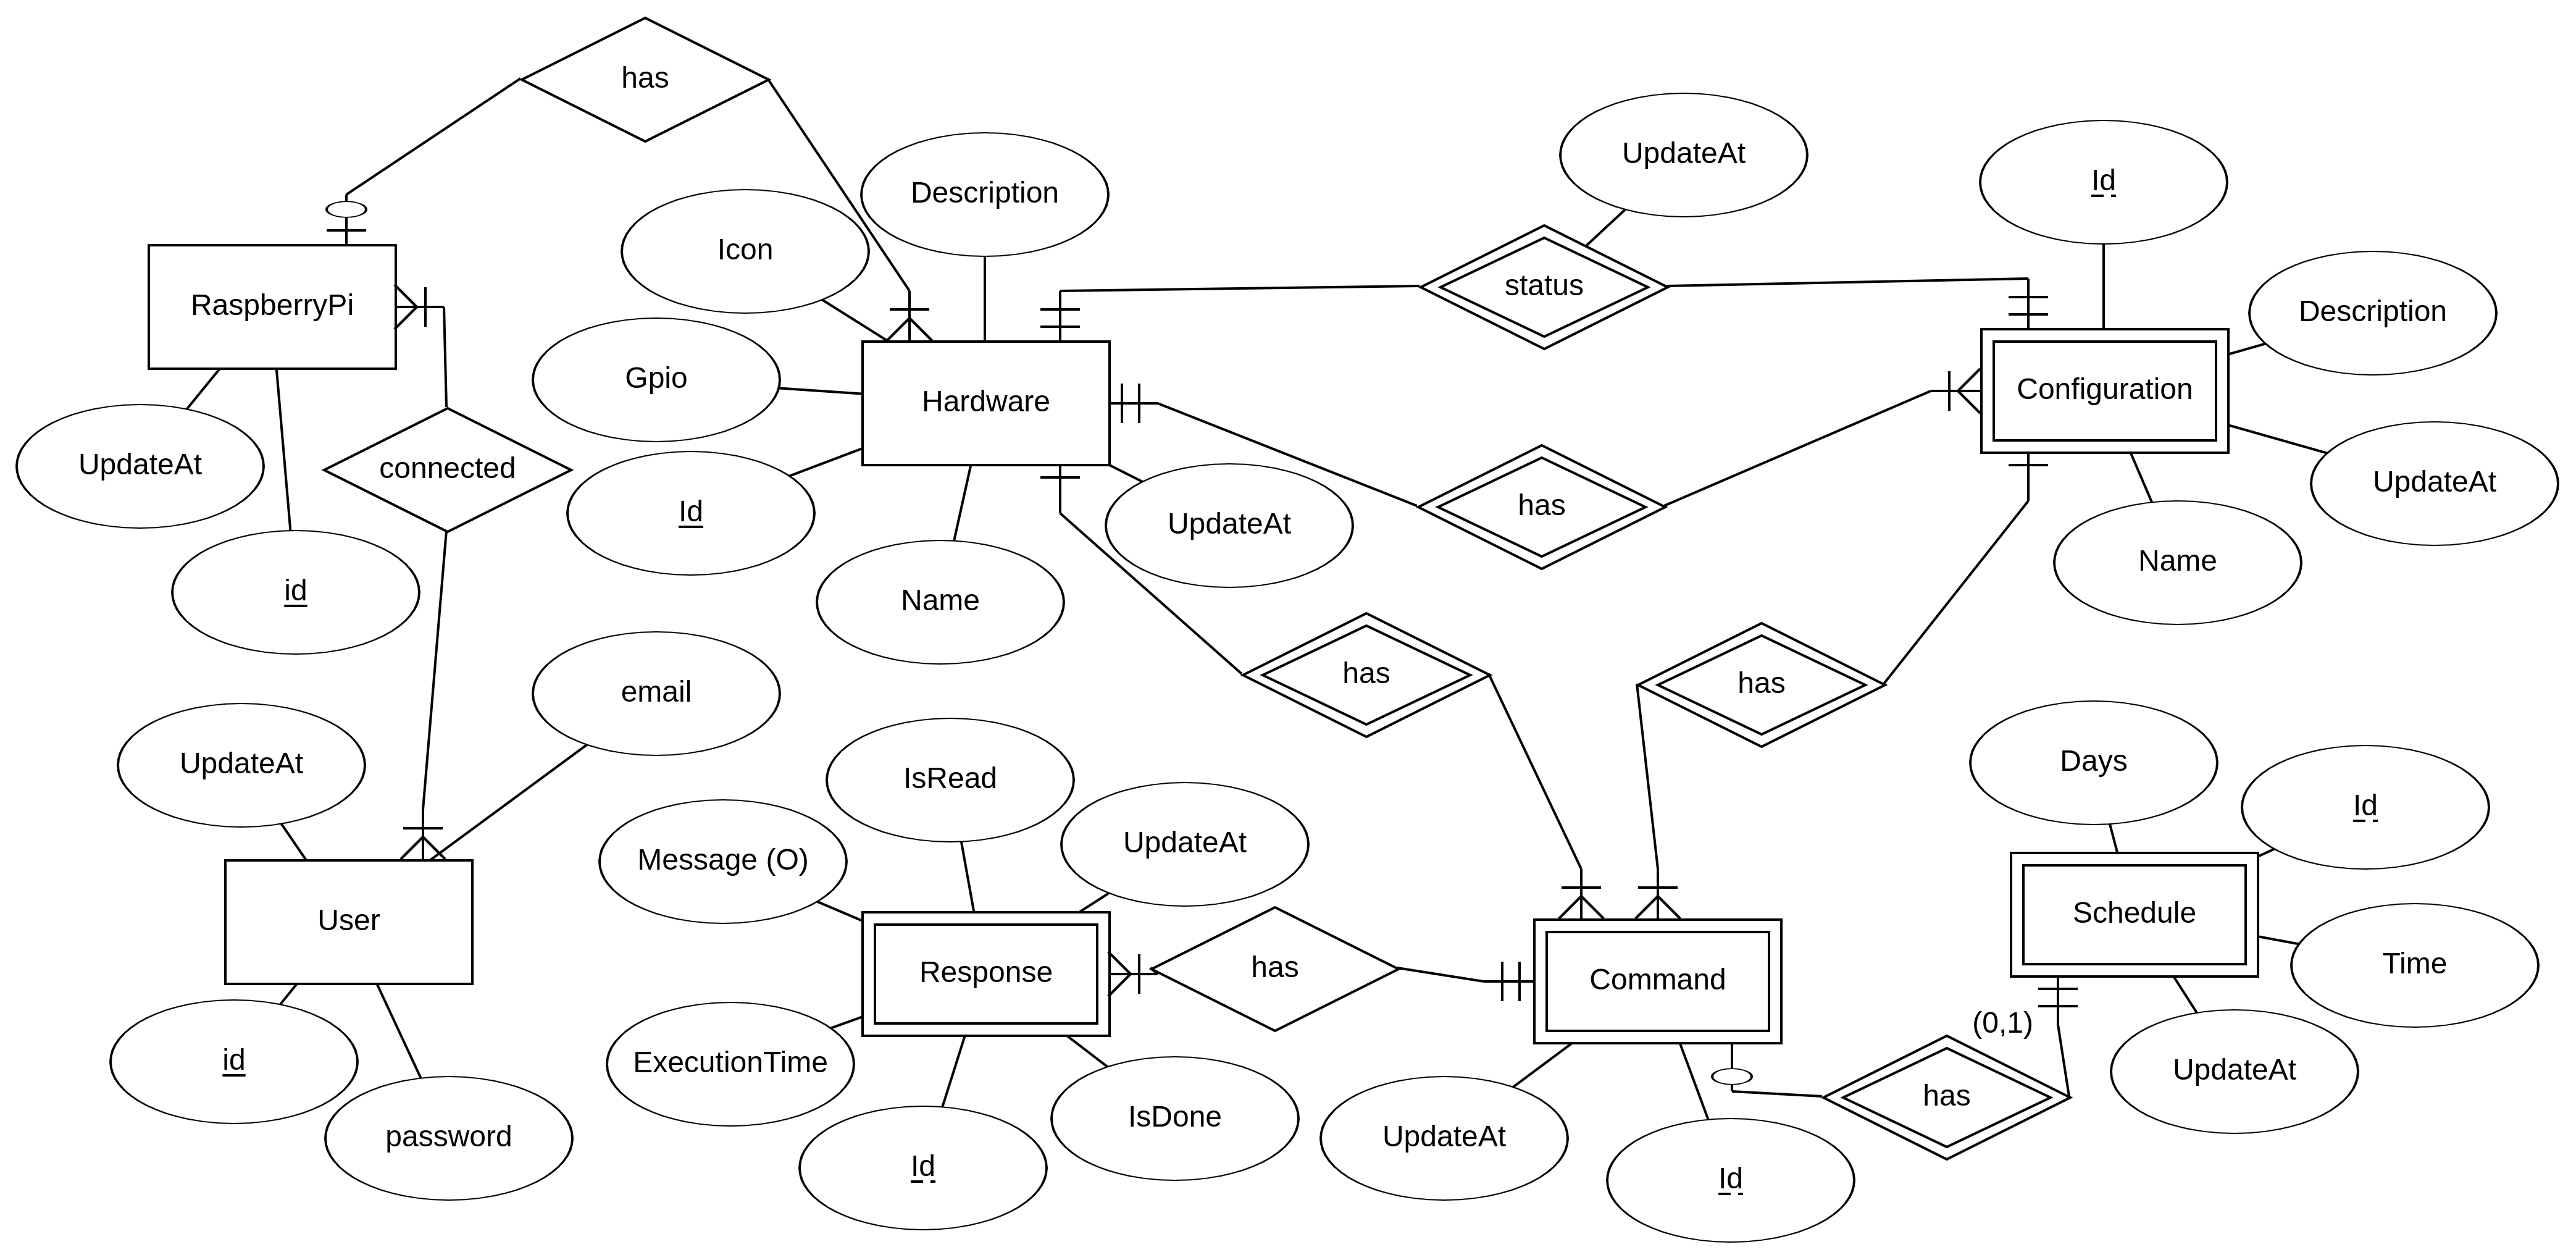
\includegraphics[width=\linewidth]{img/diagram_er1.png}
							\caption{System database}
						\end{subfigure}

						\begin{subfigure}[b]{\linewidth}
							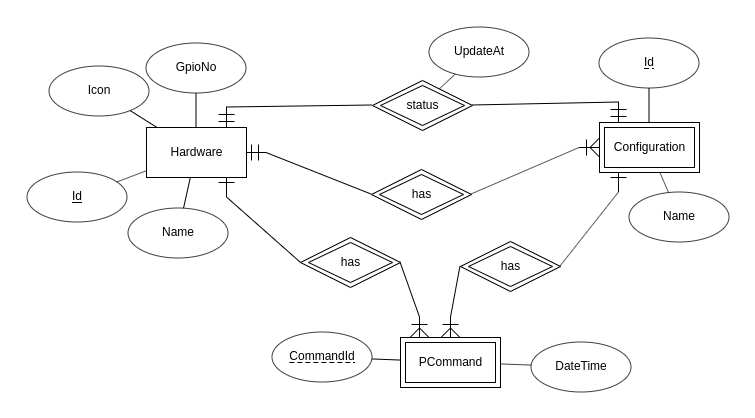
\includegraphics[width=\linewidth]{img/diagram_er2.png}
							\caption{Local queue}
						\end{subfigure}
						\caption{Entity-relationship diagrams}
					\end{figure}
				
			
				\newpage\subsubsection{Dataflow Diagram}
				\begin{figure}[H]
					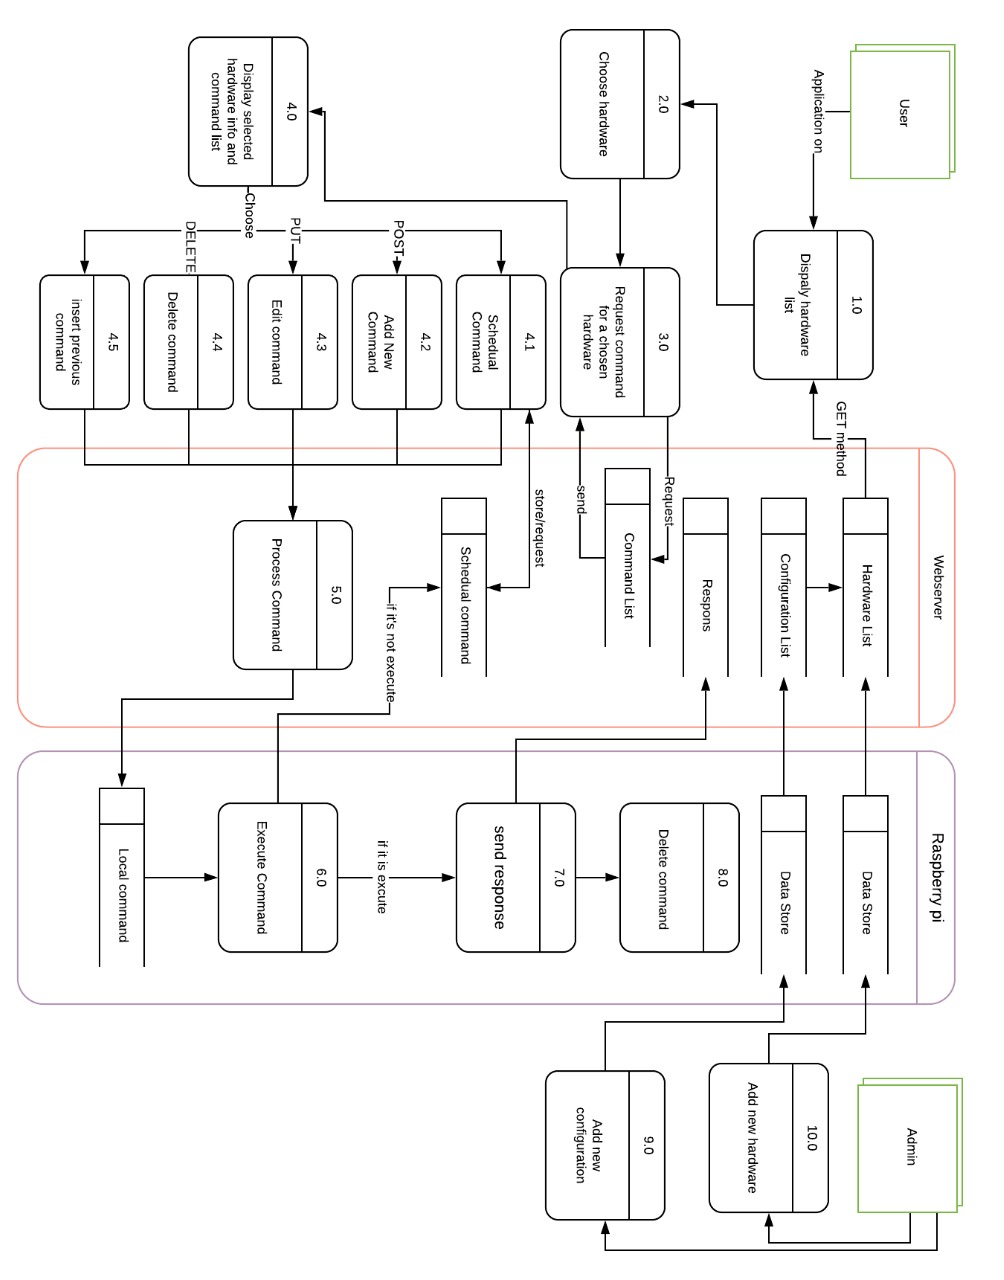
\includegraphics[width=\linewidth]{img/diagram_dataflow.jpg}
					\caption{Dataflow diagram}
				\end{figure}
				\newpage\subsection{Object-Oriented Diagrams}
				\subsubsection{Class Diagram}
					\paragraph{} \textit{Figure \ref{fig:class_web}} shows the class diagram for the web application, and \textit{figure \ref{fig:class_rp}} shows the class diagram for raspberry pi.The classes are essentially wrappers for the databases tables, except for the class \textbf{RaspberryPi}, where the functions for controlling the hardwares are.
					\paragraph{}The classes which represent database's tables inherit from a \textbf{BaseEntity} generic class. This generic class has the entity's id and \textbf{updateAt} property, which determines when the entity was created/last updated. This generic class is important as it has the methods needed to communicate with the web server. An example is \code{hardware.edit(1)}, which corresponds to the REST API \textbf{PUT} \code{/hardware/1}.
					\begin{figure}[H]
						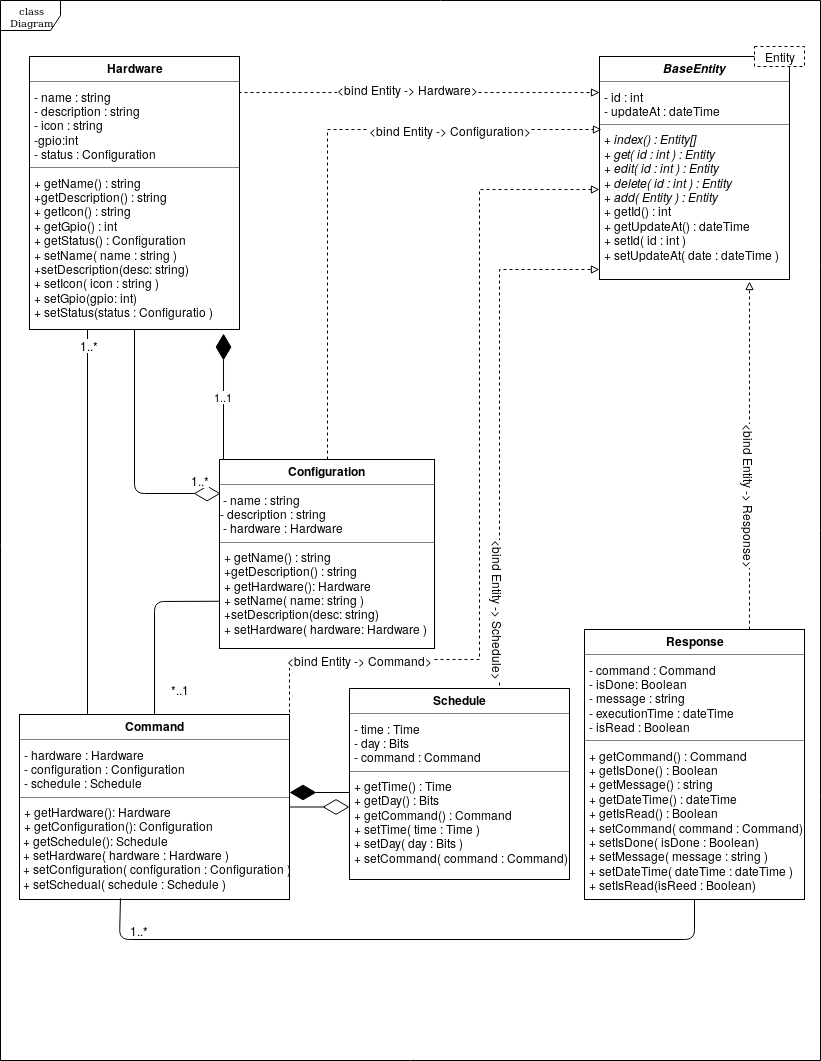
\includegraphics[width=\linewidth]{img/diagram_class1.png}
						\caption{Class diagram for the web application}
						\label{fig:class_web}
					\end{figure}
					\begin{figure}[H]
						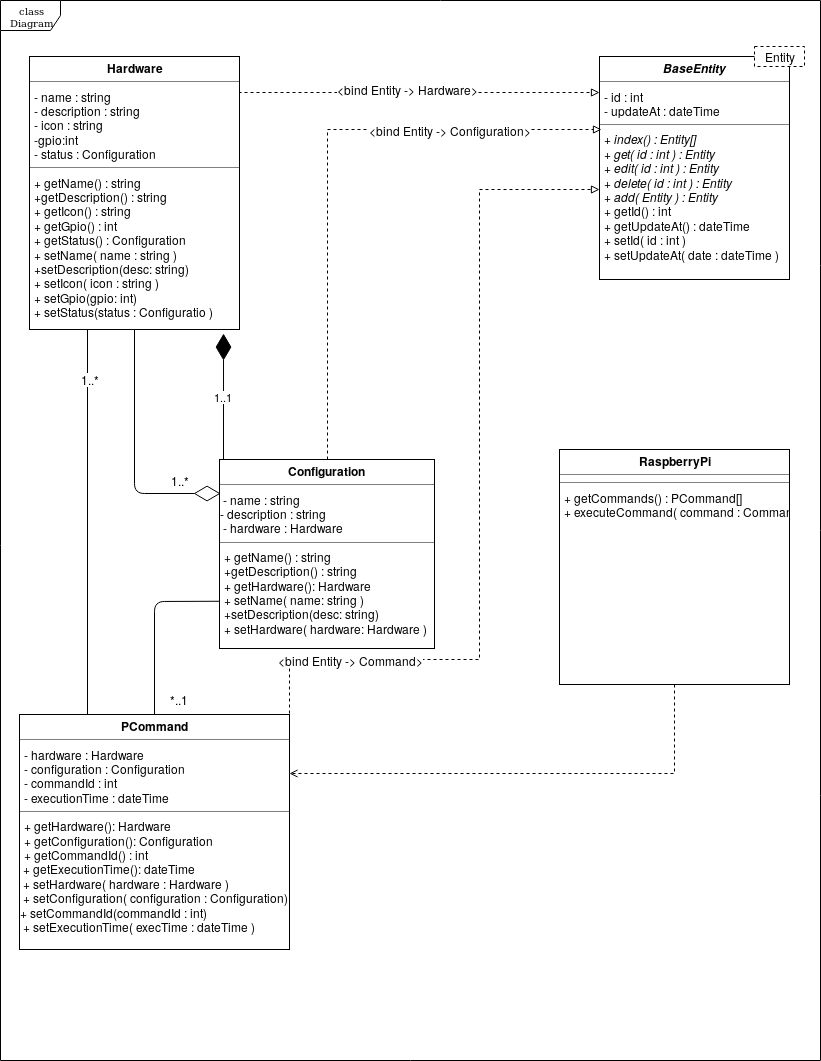
\includegraphics[width=\linewidth]{img/diagram_class2.png}
						\caption{Class diagram for the raspberry pi}
						\label{fig:class_rp}
					\end{figure}
				\newpage\subsubsection{UML representation of the REST API Diagram}
				\paragraph{} Correct calls to the web application via the REST API is the building block of our project. Thus, talking about the structure is essential. The API has 5 entities representing the database's tables. For each entity, client can use 2 methods with the entity url -e.g. \code{/hardware}-: 
				\begin{itemize}
					\item \textbf{GET}: this method corresponds to the SQL's \code{SELECT * from ...;}.
					\item \textbf{POST}: a body of type JSON is required. It holds the object attributes. This method corresponds to the SQL's \code{INSERT INTO}.
				\end{itemize} 
			 	\paragraph{}Also, client can use 3 methods with the entity url + id -e.g.\code{/hardware/6}-: 
			 	\begin{itemize}
			 		\item \textbf{GET}: this method corresponds to the SQL's \code{SELECT * from ... WHERE id = ...;}.
			 		\item \textbf{PUT}: a body of type JSON is required. It holds the object attributes. This method corresponds to the SQL's \code{UPDATE ... WHERE id = ..;}.
			 		\item \textbf{DELETE}: this method corresponds to the SQL's \code{DELETE FROM ... WHERE id = ..;}.
			 	\end{itemize} 
		 		\textit{Figure \ref{fig:rest} shows the API's hierarchy and figure \ref{fig:rest_model} shows the models. For full documentation see Appendix \ref{appendix:api_doc}}
				\begin{figure}[H]
					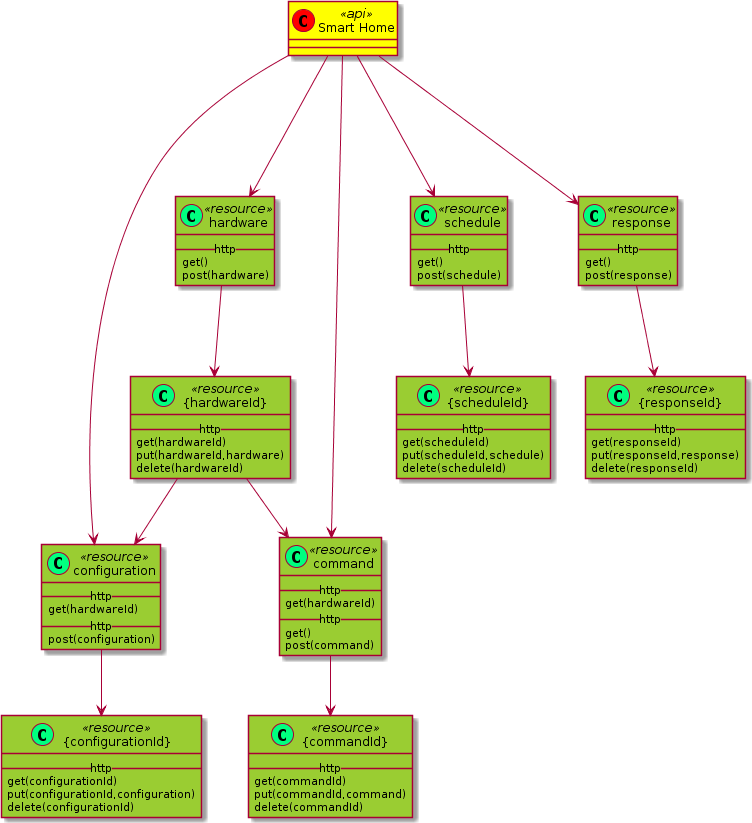
\includegraphics[width=\linewidth]{img/rest_uml.png}
					\caption{REST API}
					\label{fig:rest}
				\end{figure}
			\begin{figure}[H]
				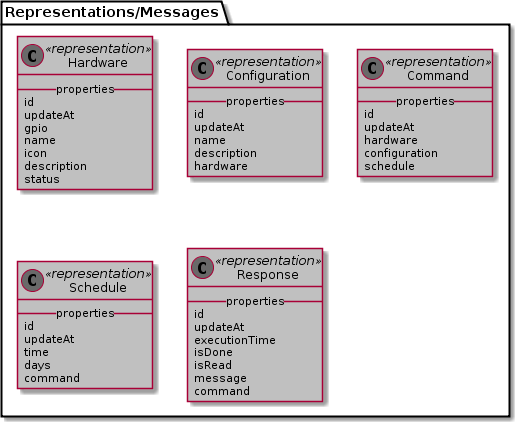
\includegraphics[width=\linewidth]{img/rest_uml_model.png}
				\caption{REST API models}
				\label{fig:rest_model}
			\end{figure}	
		\newpage

			
	\mychapter{System Design}
		\section{System Architecture}
		\paragraph{} The proposed project has 4 tiers. The Android App, the web app and finally the raspberry pi script and finally the system database. The android app works as the user interface. The raspberry pi app is the one responsible for controlling the actual hardwares. The web app  works as a medium for managing user requests and raspberry pi's response. Finally, the database that stores these data. \textit{Figure \ref{fig:diagrm_component} and figure \ref{fig:diagram_deployment} show the architecture for the system using component and deployment diagrams.}
		\subsection{The android application}
		\paragraph{} Also known as the client tier. It enables the user to interact with the system through a simple graphical user interface. Android application can send requests to the web server and receive responses. This app is designed using Java programming language, Android framework, Retrofit library for managing networking and finally Gson for parsing JSON responses.
		\subsection{The raspberry pi script}
		\paragraph{} Also known as the aggregation tier. It executes the commands and send responses to the web application. The script is a simple python program that controls different hardwares using GPIO library. 
		\subsection{The web application}
		\paragraph{} Also known as the delivery tier. It works as an immediate medium between the user and raspberry pi. The advantage for adding this layer is guaranteed execution regardless of user location and distance from raspberry pi. The web app will be deployed on an ubuntu server. It is made using python programming language and flask framework. Also, sqlalchemy, which is an ORM for managing database interaction, will be used to ease the development. 
		\subsection{The system database}
		\paragraph{} Also known as the Services tier. It manages and stores all system data.
		\begin{figure}[H]
			\centering
			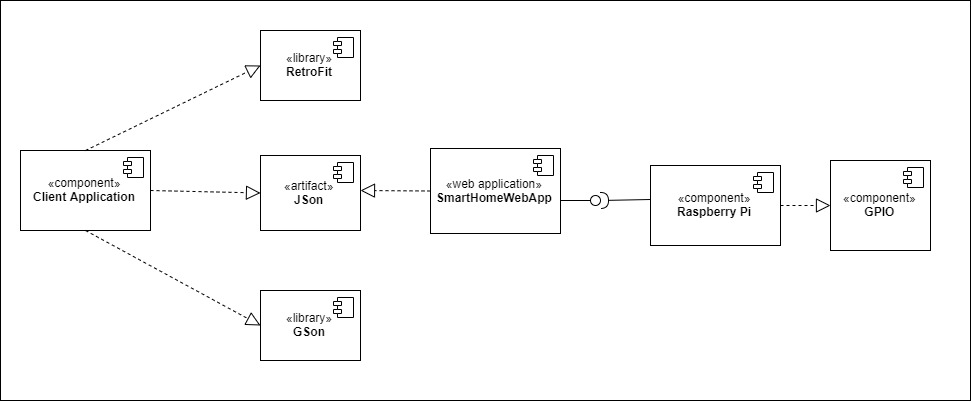
\includegraphics[width=\linewidth]{img/diagram_component.jpg}
			\caption{Component Diagram}
			\label{fig:diagrm_component}
		\end{figure}
		\begin{figure}[H]
			\centering
			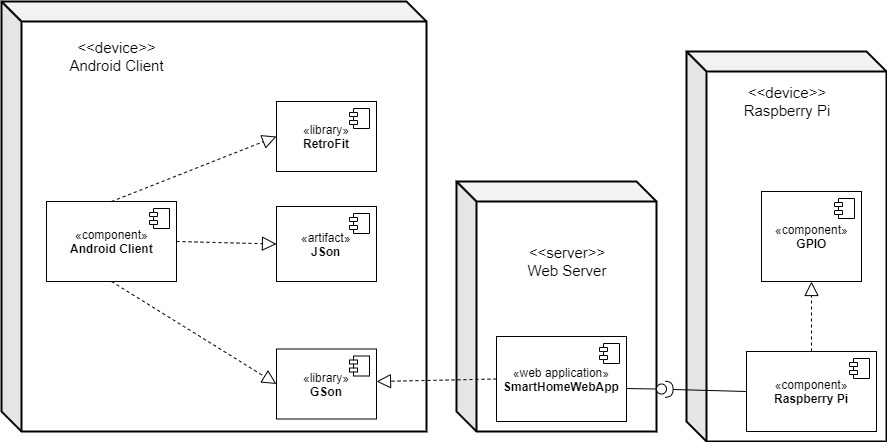
\includegraphics[width=\linewidth]{img/diagram_deployment.jpg}
			\caption{Deployment Diagram}
			\label{fig:diagram_deployment}
		\end{figure}
		\paragraph{} \textit{Figure \ref{fig:diagram_architecture}} shows the four-tier architecture explained above. In our system, the best architecture to use is four-tier architecture because of it is flexibility and scalability to add multiple services. Also, it adopts users’ experiences that are fast, responsive, and tailored unique needs. Furthermore, multi-tier architecture also reduces traffic on the network\cite{architecture}.
		\begin{figure}[H]
			\centering
			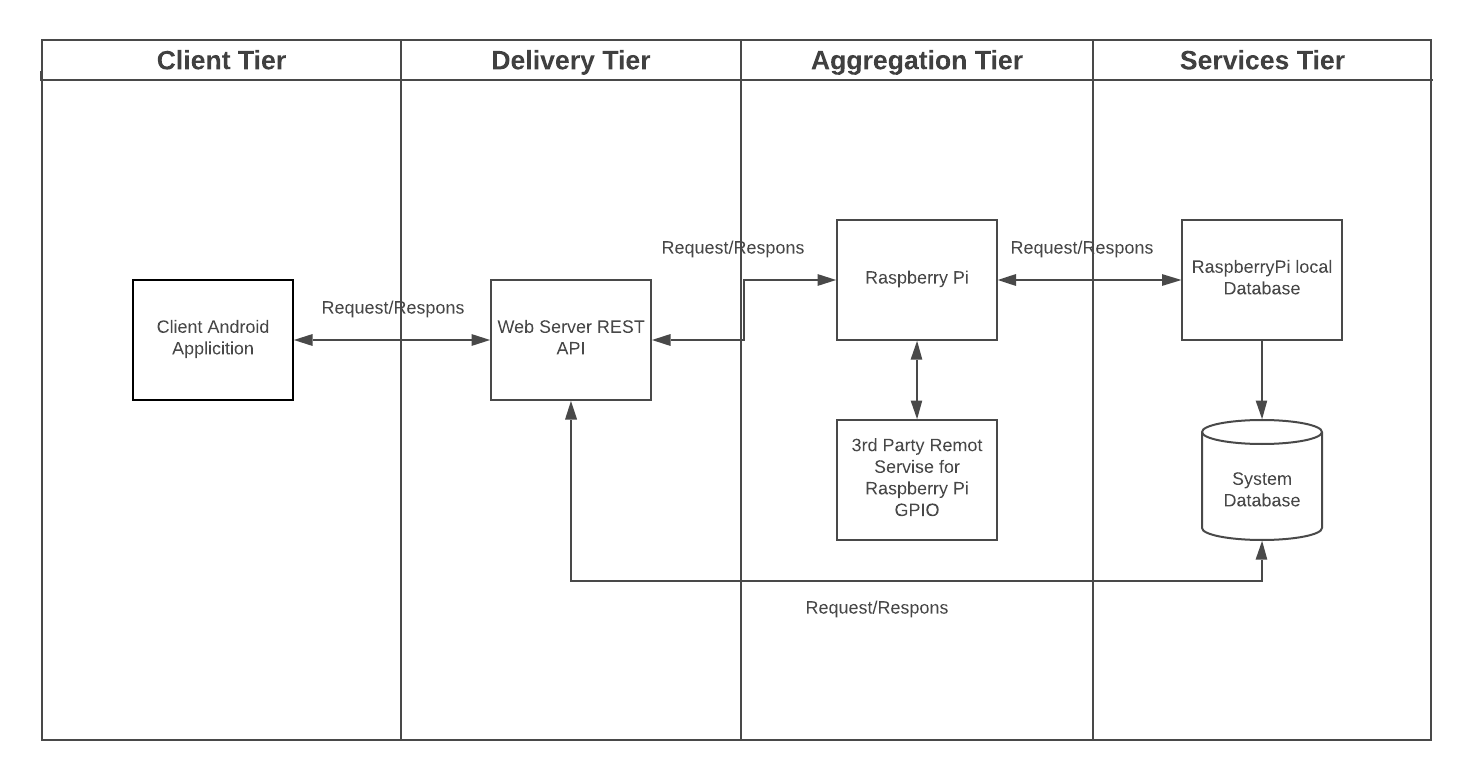
\includegraphics[width=\linewidth]{img/diagram_architecture.png}
			\caption{Architecture Diagram}
			\label{fig:diagram_architecture}
		\end{figure}
		\newpage\section{User Interface Design}
		\subsection{Login Activity}
		\paragraph{} \textit{Figure \ref{fig:activity_login}} shows the login activity. It is the activity that the user will see when the app is first launched to prompt the user to enter their credentials.
		\begin{figure}[H]
			\centering
			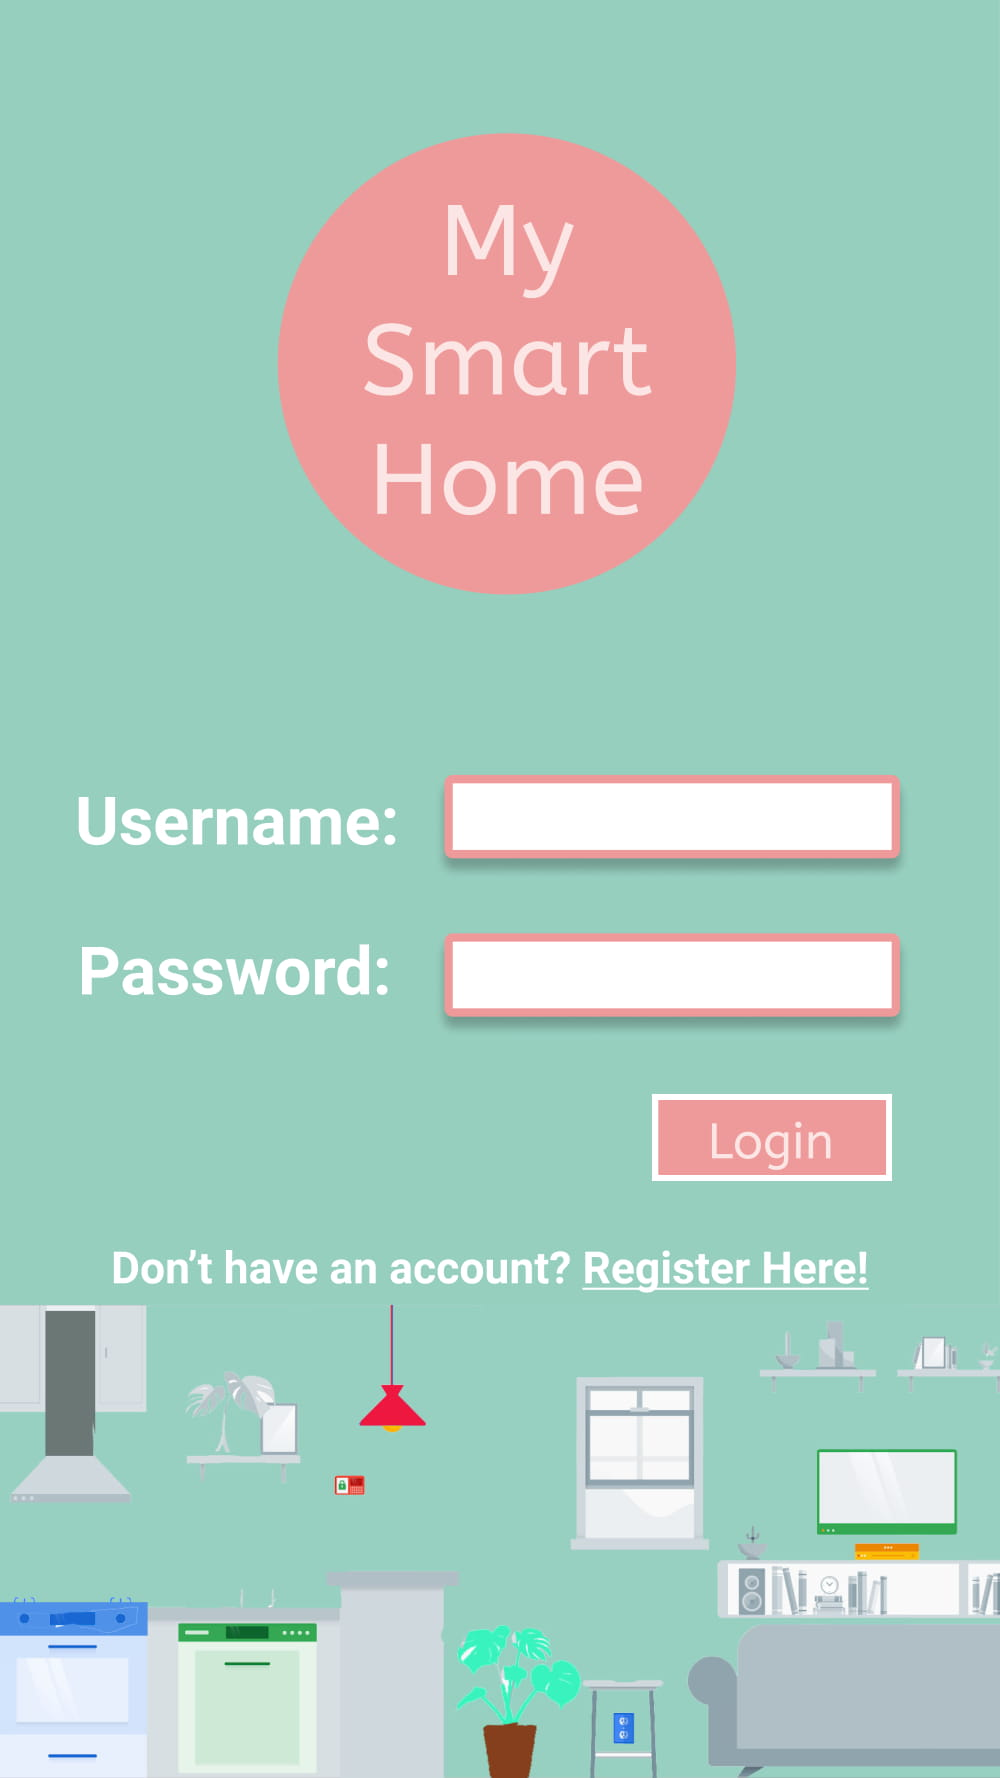
\includegraphics[width=.5\linewidth]{img/activity_login1.jpg}
			\caption{UI: Login Activity}
			\label{fig:activity_login}
		\end{figure}
		\newpage\subsection{Raspberry Activity}
		\paragraph{} \textit{Figure \ref{fig:activity_raspberry}} shows the raspberry activity. All the raspberry connected to the user shall be viewed here, with the option of deleting them or adding new ones.
		\begin{figure}[H]
			\centering
			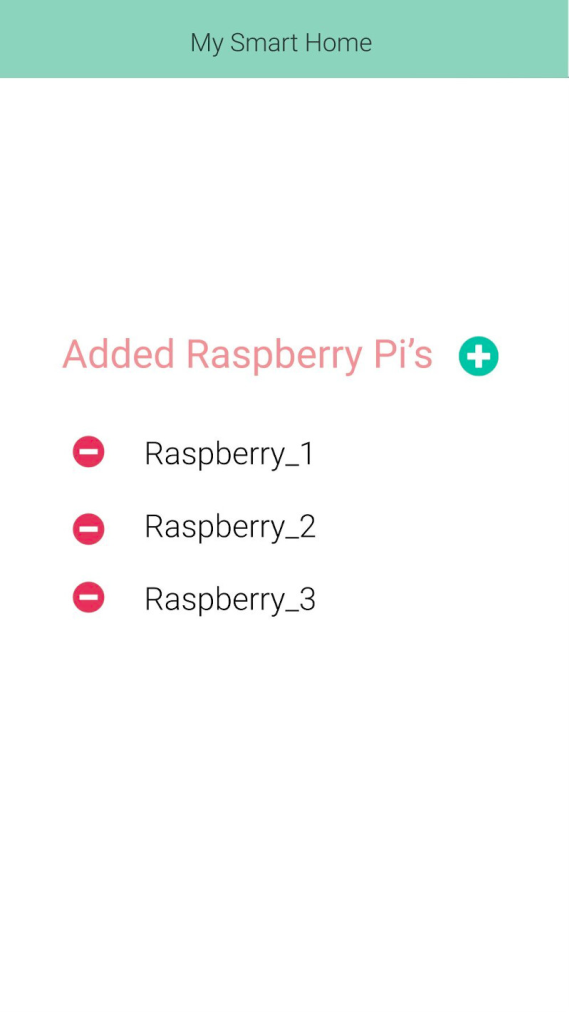
\includegraphics[width=.5\linewidth]{img/activity_raspberry.png}
			\caption{UI: Raspberry Activity}
			\label{fig:activity_raspberry}
		\end{figure}
		\newpage\subsection{Hardwares Activity}
		\paragraph{} \textit{Figure \ref{fig:activity_home}} shows the hardwares activity.  All the hardwares in the system shall be displayed in a grid.
		\begin{figure}[H]
			\centering
			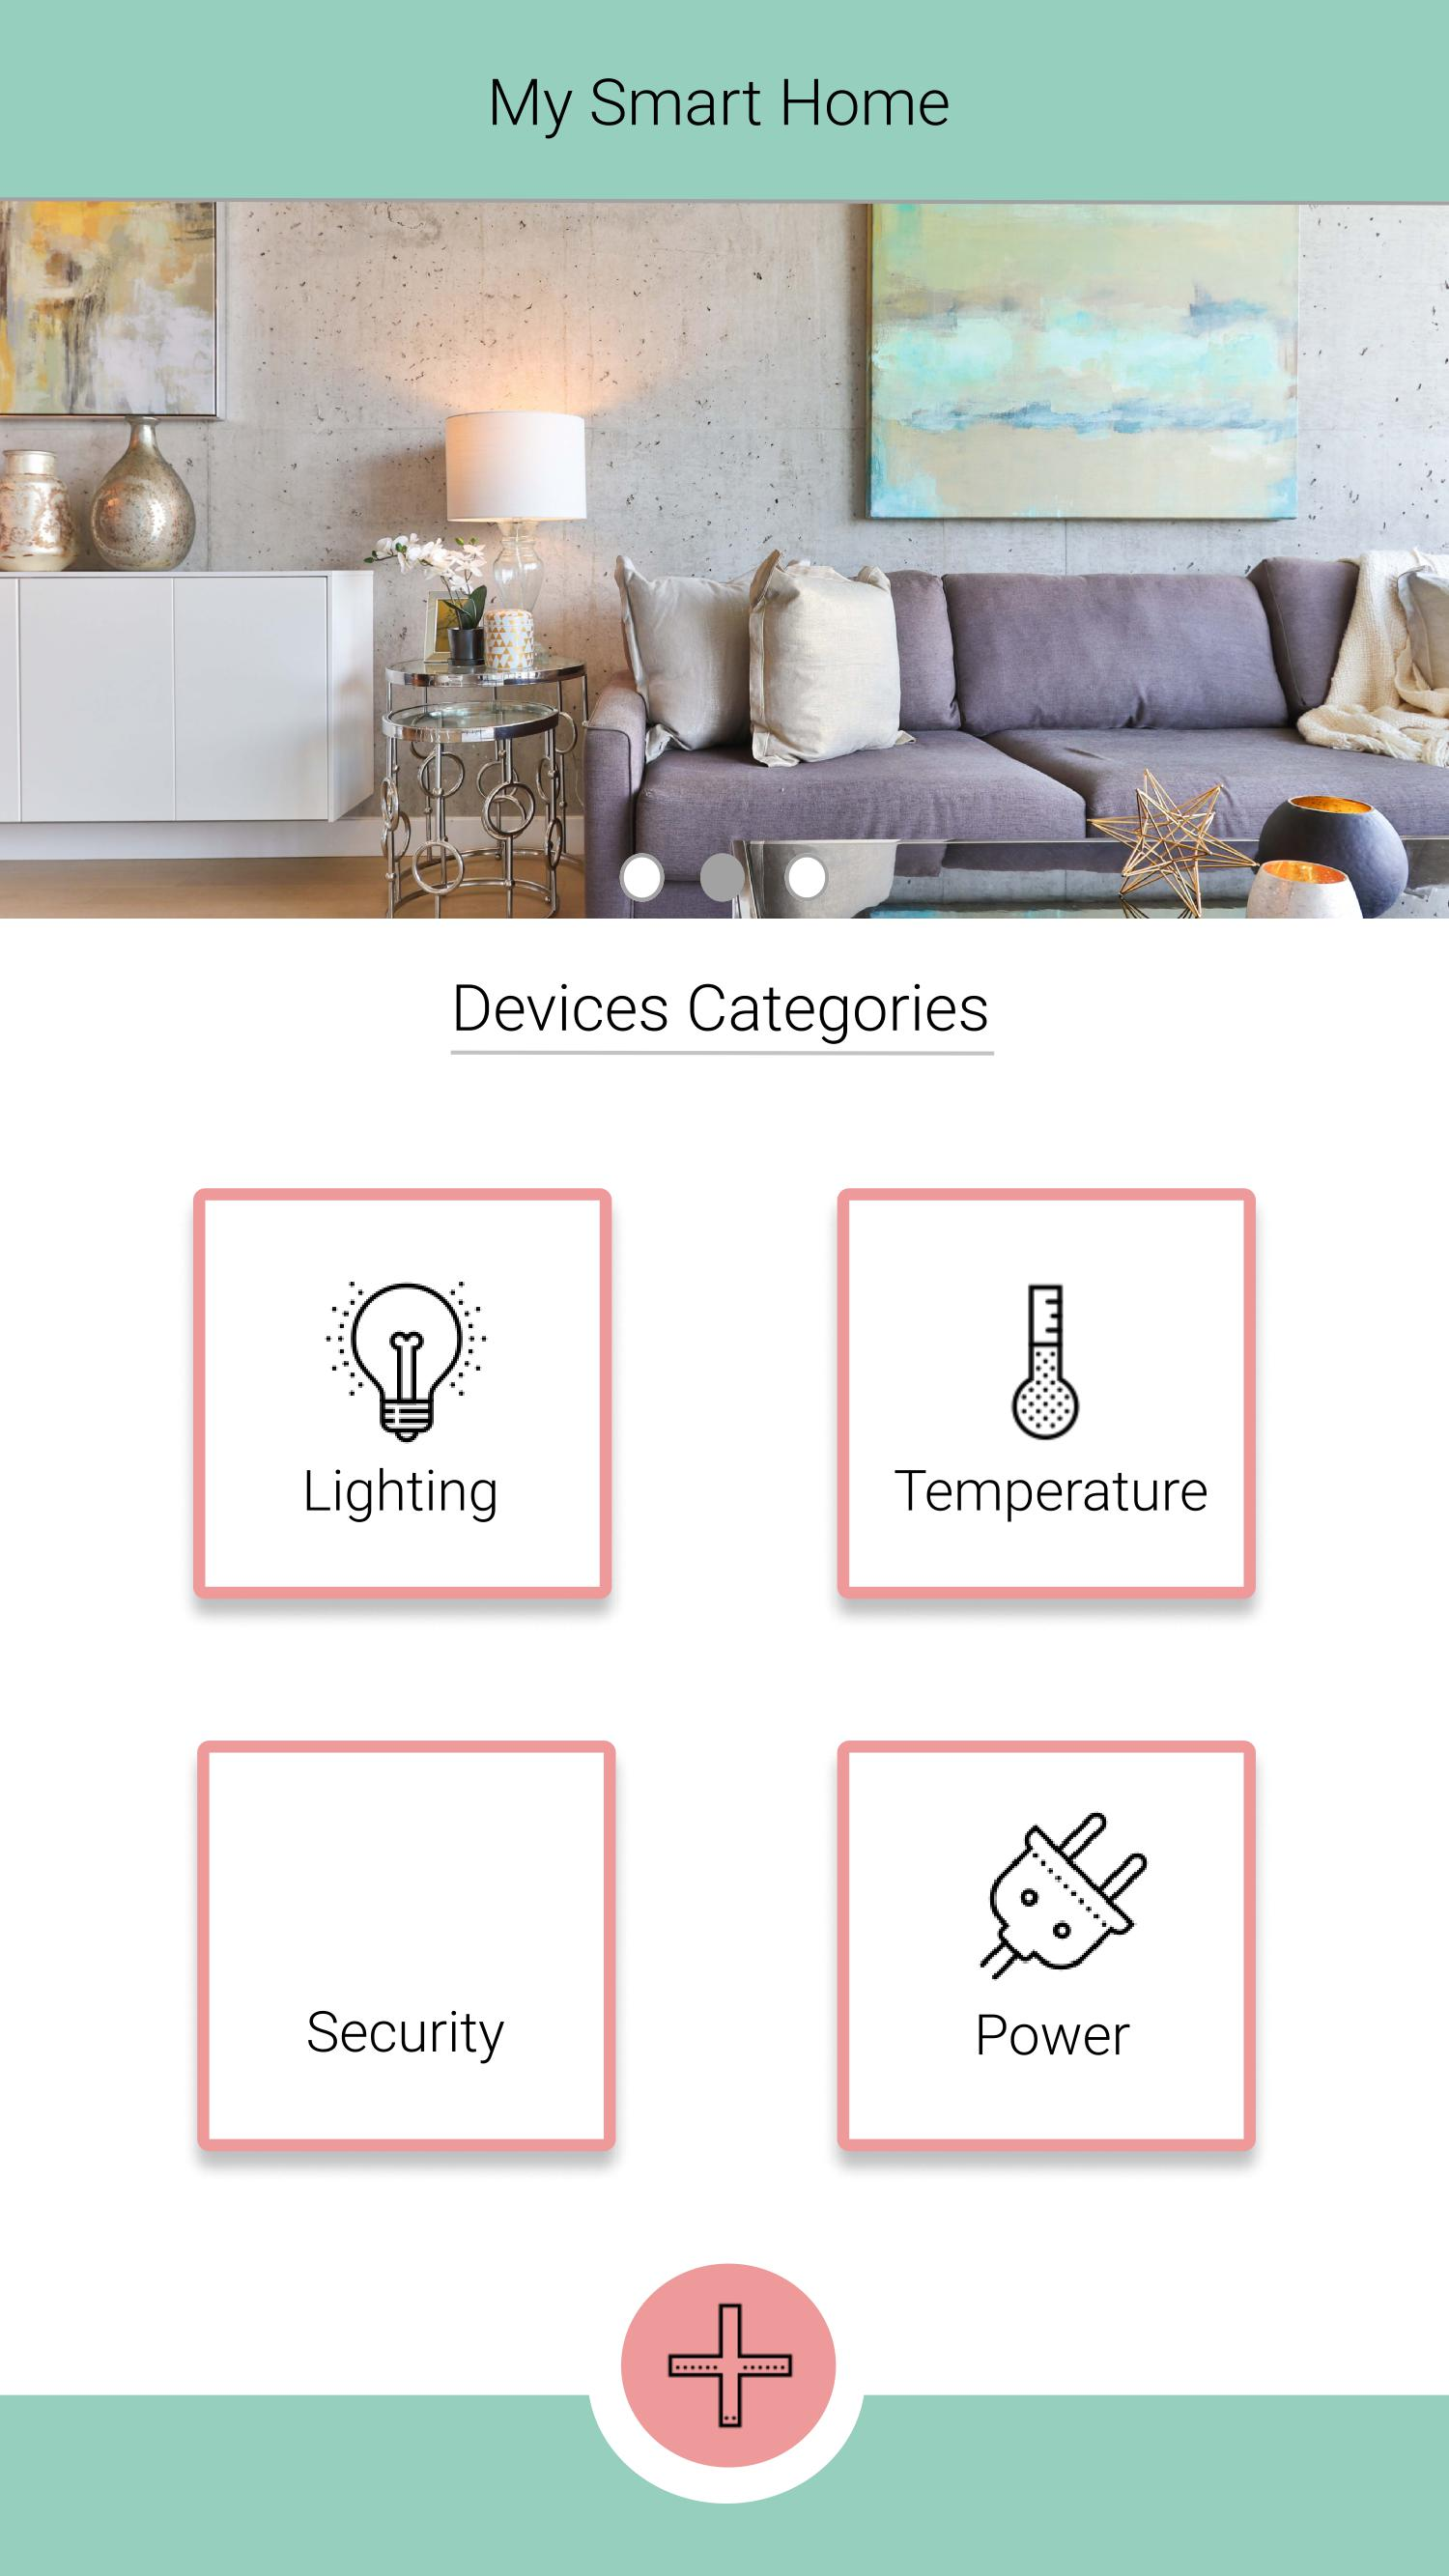
\includegraphics[width=.5\linewidth]{img/activity_home.jpg}
			\caption{UI: Home Activity}
			\label{fig:activity_home}
		\end{figure}
		\newpage\subsection{Hardware Activity}
		\paragraph{} \textit{Figure \ref{fig:activity_hardware}} shows the hardware activity. The user first is shown the current status for the hardware. Then, a list of active command is presented with the ability to edit/delete each command. Also, the user can click on the \textit{+} icon to add a new command.
		\begin{figure}[H]
			\centering
			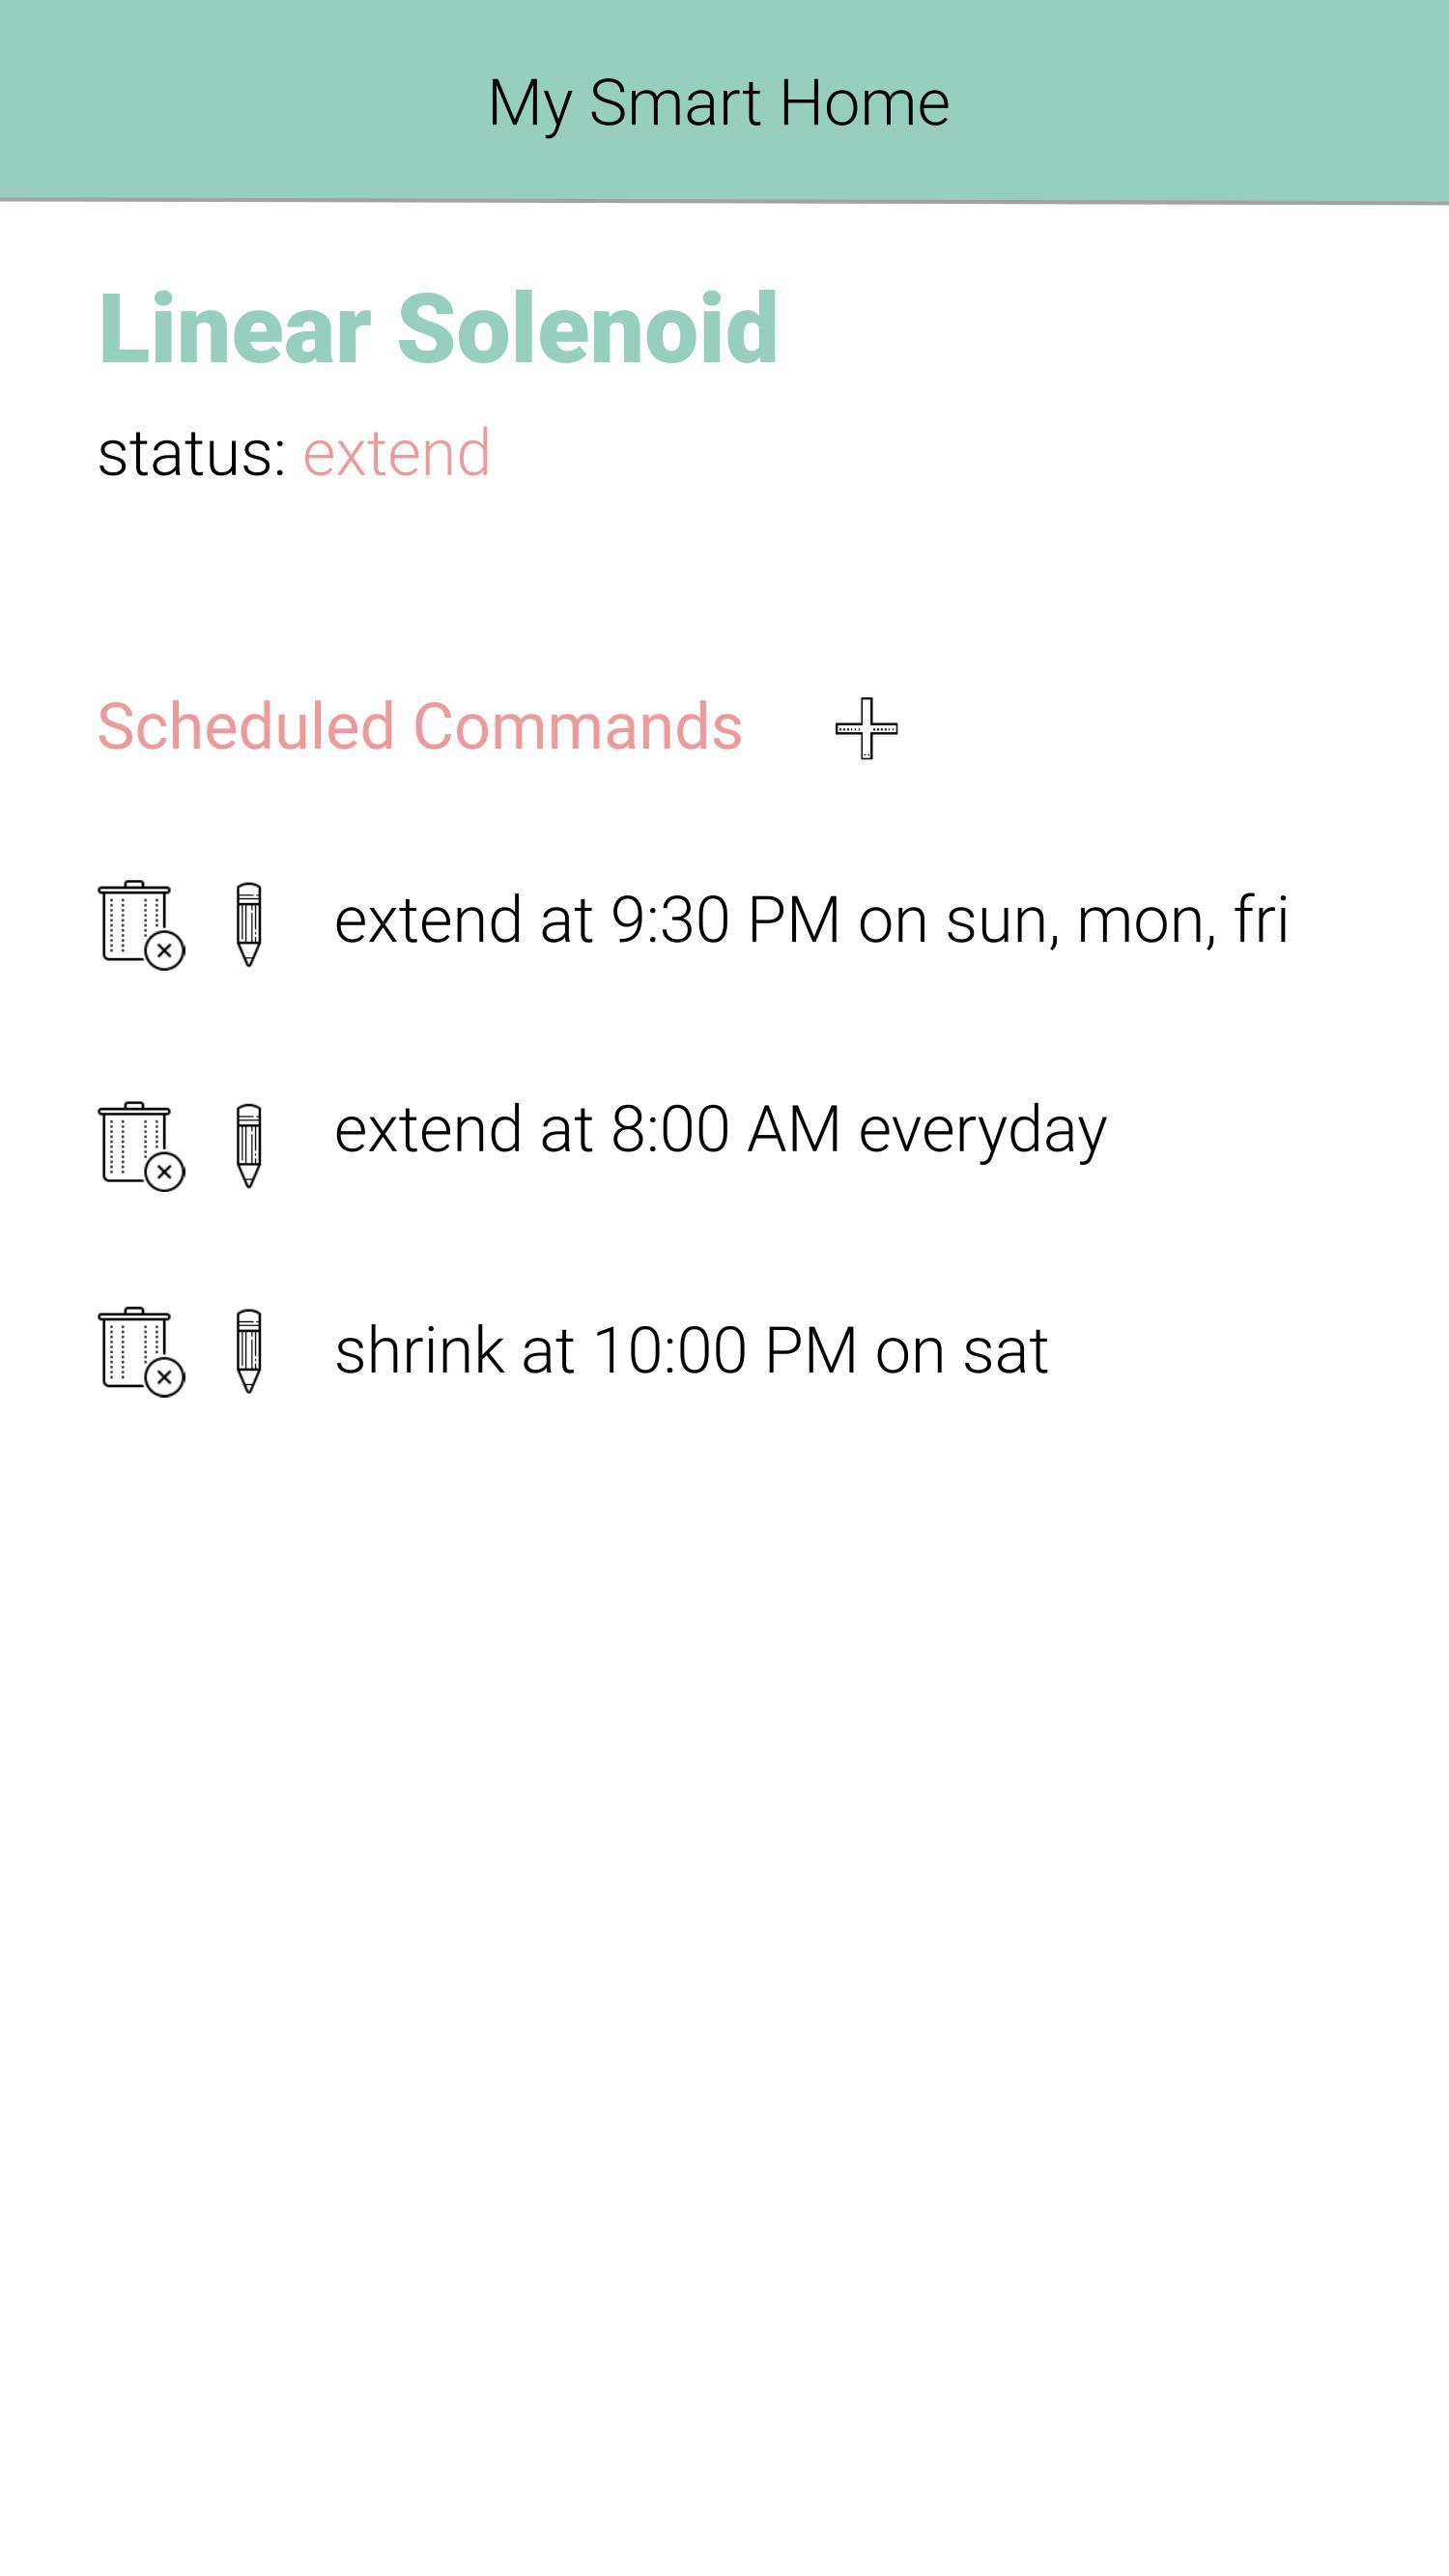
\includegraphics[width=.5\linewidth]{img/activity_hardware.jpg}
			\caption{UI: Hardware Activity}
			\label{fig:activity_hardware}
		\end{figure}
		\newpage\subsection{New Command Activity}
		\paragraph{} \textit{Figure \ref{fig:activity_new_command}} shows the new command activity, where the user can add a new command to be executed. First, the user choose the configuration wanted. Then either execute the command now, or click on the schedule, which will open a new activity to choose the scheduling information desired.
		\begin{figure}[H]
			\centering
			\includegraphics[width=.5\linewidth]{img/activity_new_command.jpg}
			\caption{UI: New Command Activity}
			\label{fig:activity_new_command}
		\end{figure}
		\newpage\subsection{Schedule Activity}
		\paragraph{} \textit{Figure \ref{fig:activity_schedule}} shows the schedule activity. This activity appears once the user clicks on add schedule in the previous activity. The user can choose the time of execution and the days to execute the action here.
		\begin{figure}[H]
			\centering
			\includegraphics[width=.5\linewidth]{img/activity_schedule.jpg}
			\caption{UI: Schedule Activity}
			\label{fig:activity_schedule}
	\end{figure}
		\newpage\subsection{Progress Fragment}
		\paragraph{} \textit{Figure \ref{fig:activity_progress}} shows the waiting progress fragment that will appear until the web server respond with the code \code{201}, which denotes a successful creation of a command.
		\begin{figure}[H]
			\centering
			\includegraphics[width=.5\linewidth]{img/activity_progress.jpg}
			\caption{UI: Progress Fragment}
			\label{fig:activity_progress}
		\end{figure}
		\newpage\subsection{Message Fragment}
		\paragraph{} Once the server respond, the message embedded with the response shall be displayed to the user. Either \textbf{Done!} with \code{201} or the error message when the code is different. \textit{Figure \ref{fig:activity_done}} shows the message when the command is successfully created.
		\begin{figure}[H]
			\centering
			\includegraphics[width=.5\linewidth]{img/activity_done.jpg}
			\caption{UI: Message Fragment}
			\label{fig:activity_done}
		\end{figure}
	\begin{comment}
		\newpage	
	\chapter{Implementation}
		\section{Implementation}
		\section{Implementation Requirements}
			\subsection{Software Requirements}
			\subsection{Hardware Requirements}
		\section{Implementation Detailed}
		\section{I/O Screens}
		\newpage	
	\chapter{Testing}
		\section{Testing}
		\section{Test Plan}
			\subsection{Unit Test}
			\subsection{Functional Test}
			\subsection{Acceptance Test}
		\section{Test Items}
			\subsection{Features to Be Tested}
			\subsection{Schedule of Test Actions}
			\subsection{Test Tasks}
		\section{Test Case}
		\section{Test Result}
		\newpage	
	\chapter{Conclusion}
		\section{Conclusion}
		\section{Evaluation}
		\section{Future Work}
	\newpage
	
	
	
	\end{comment}
	\bibliographystyle{ieeetr}
	\renewcommand{\bibname}{References}
	\bibliography{References}


	\clearpage
	\mychapter{Appendices}
	\appendix
	%\renewcommand{thesection}{\Alph{section}}
		\chapter{Figures}
		\label{appendix:similar_system_comparision}
		\section{Similar systems hub design}
		\begin{figure}[H]
			\begin{subfigure}[b]{.5\linewidth}
				\includegraphics[width=\linewidth]{img/insteon_hw.png}
				\caption{Insteon}
			\end{subfigure}
			\begin{subfigure}[b]{.5\linewidth}
				\includegraphics[width=\linewidth]{img/wink_hw.png}
				\caption{Wink}
			\end{subfigure}
			\begin{subfigure}[b]{.5\linewidth}
			\includegraphics[width=\linewidth]{img/samsung_hw.png}
				\caption{Samsung}
			\end{subfigure}
			\begin{subfigure}[b]{.5\linewidth}
				\includegraphics[width=\linewidth]{img/raspberry.png}
				\caption{Raspberry Pi}
			\end{subfigure}
			\caption{Similar systems: hub design}
		\end{figure}

		\newpage\chapter{REST API Documentation}
		\label{appendix:api_doc}
		\includepdf[pages=-, width=\linewidth, pagecommand={\pagestyle{fancy}}]{file/api-documentation.pdf}

\end{document}


	\begin{comment}
	TODO:
	# Doha data flow
	# all functions
	\end{comment}
